~\section*{Binning in muon+jets channel}
\label{as:binning_muon}

\begin{figure}[hbtp]
    \centering
     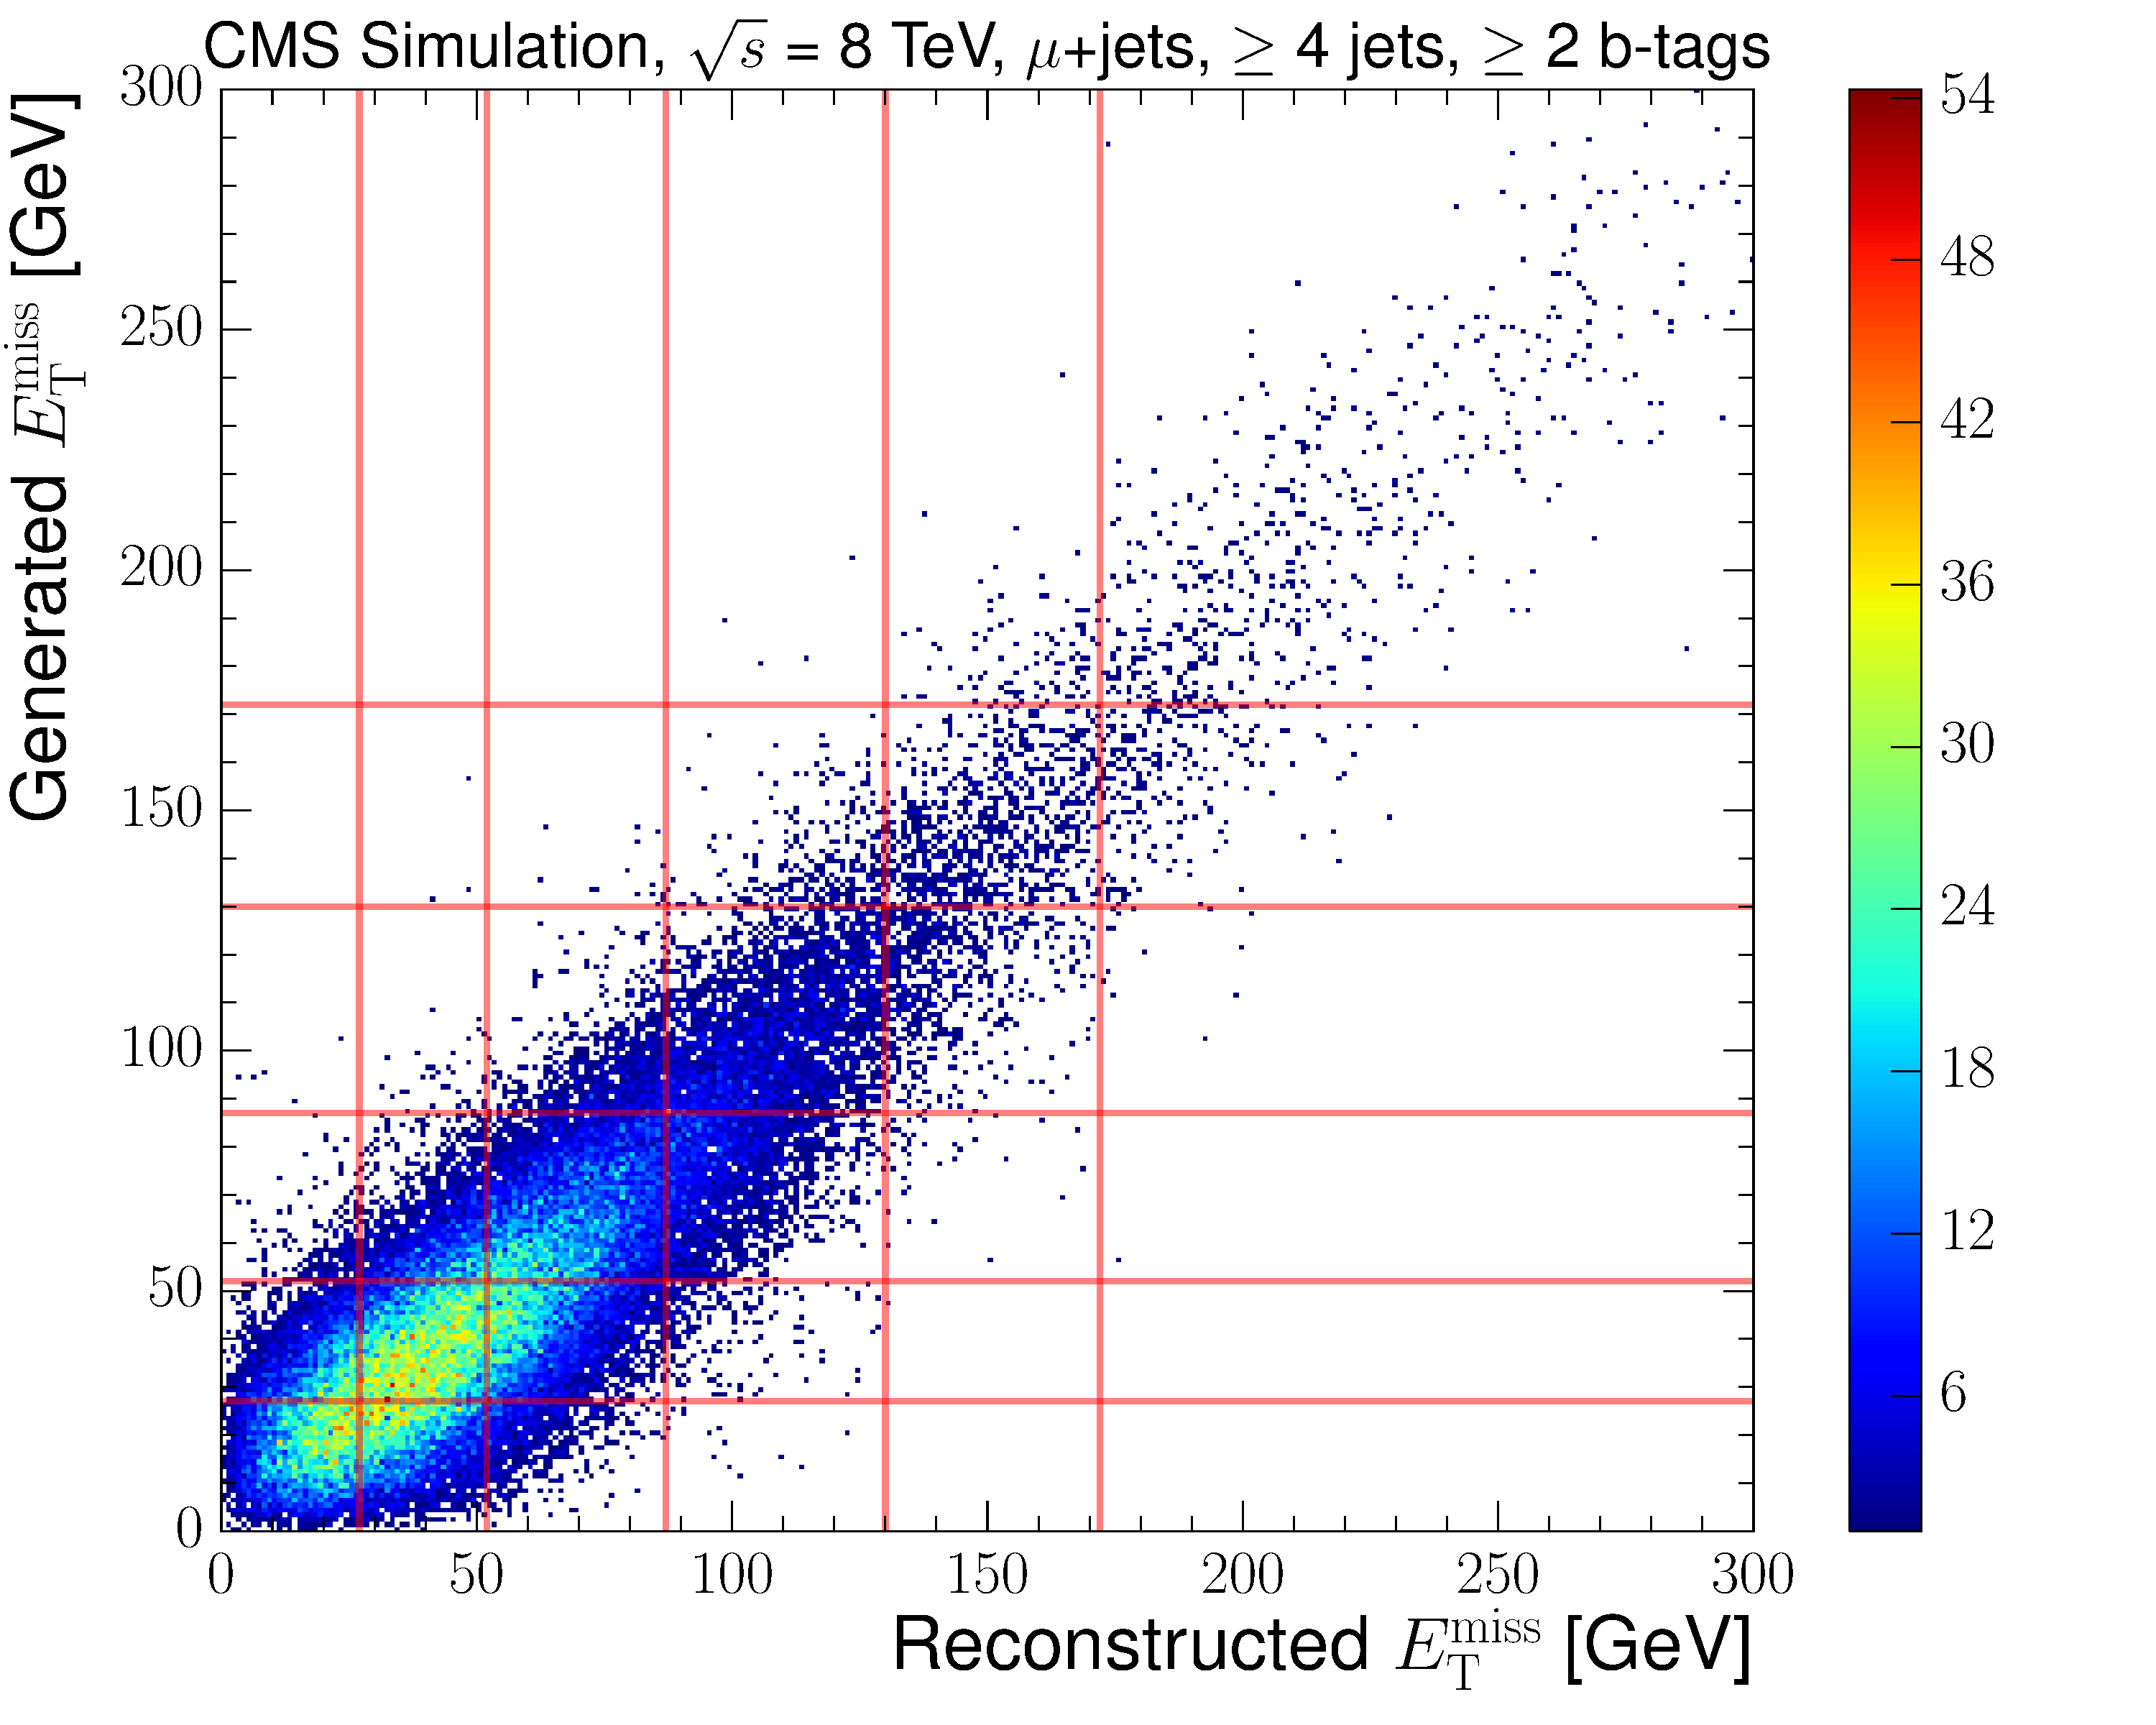
\includegraphics[width=0.48\textwidth]{Chapters/04_Analysis/04b_XSections/images/binning/muon_MET_8TeV.pdf}\hfill
     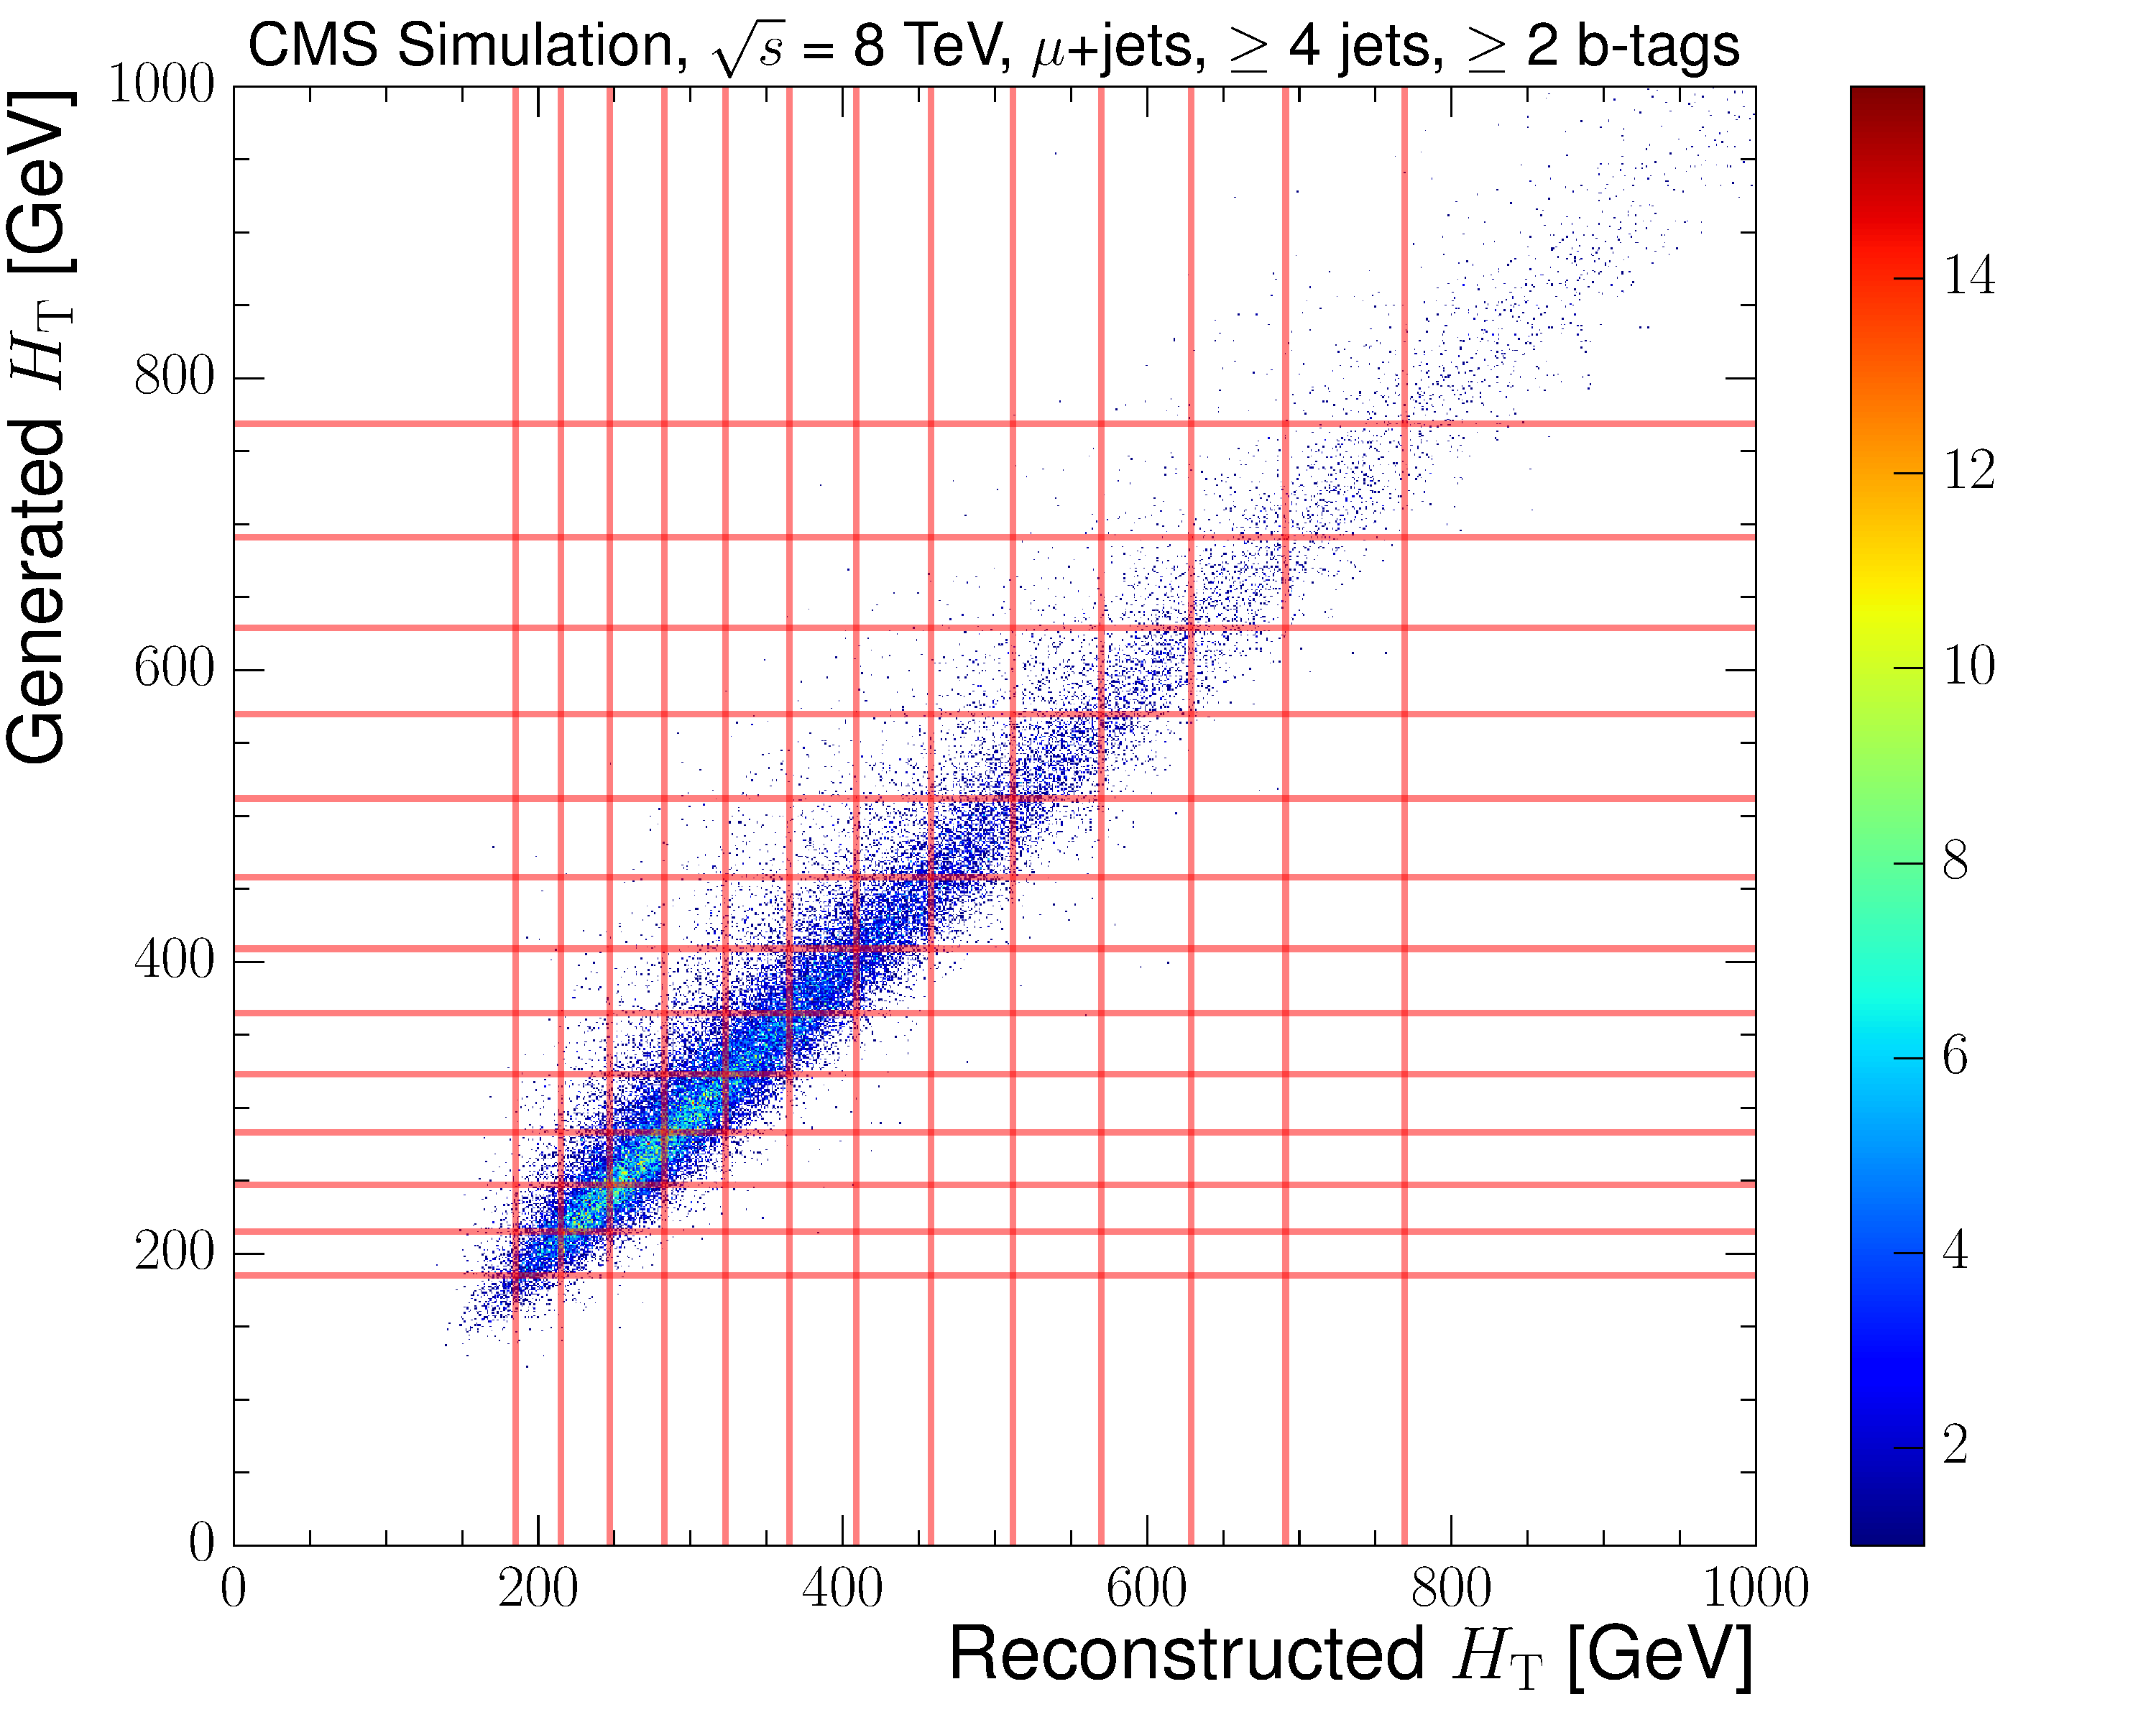
\includegraphics[width=0.48\textwidth]{Chapters/04_Analysis/04b_XSections/images/binning/muon_HT_8TeV.pdf}\\
     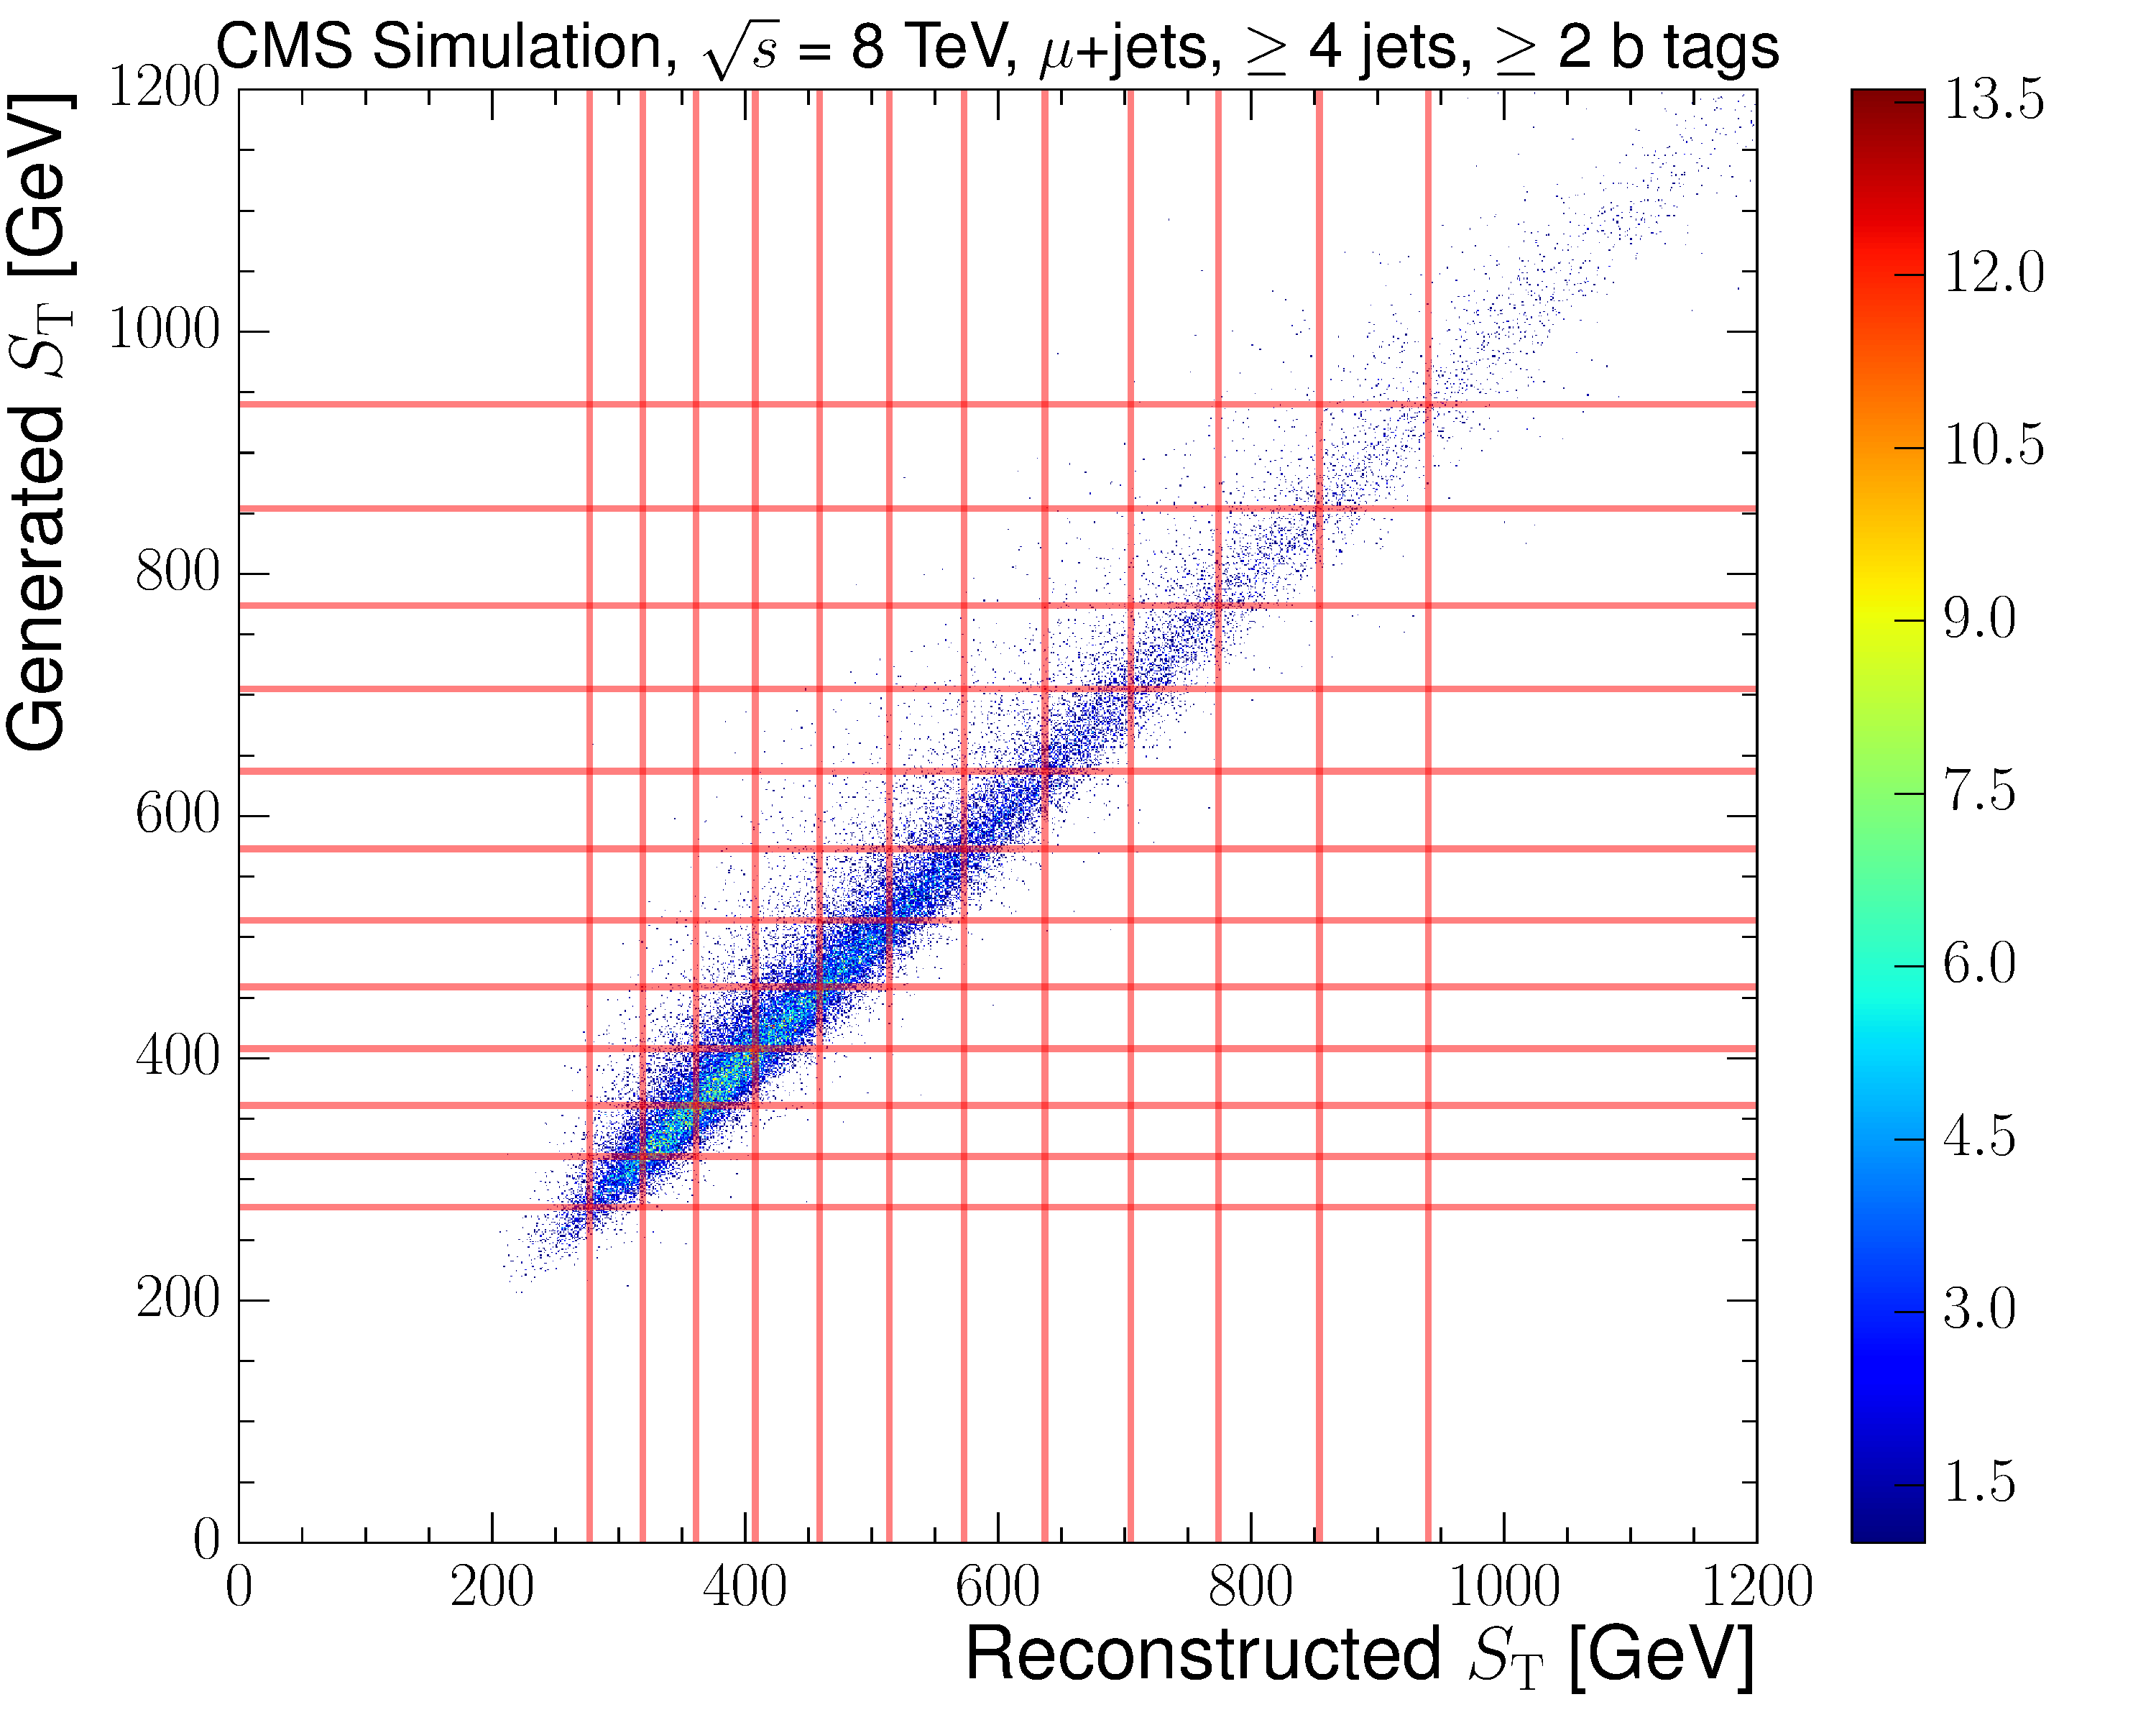
\includegraphics[width=0.48\textwidth]{Chapters/04_Analysis/04b_XSections/images/binning/muon_ST_8TeV.pdf}\hfill
     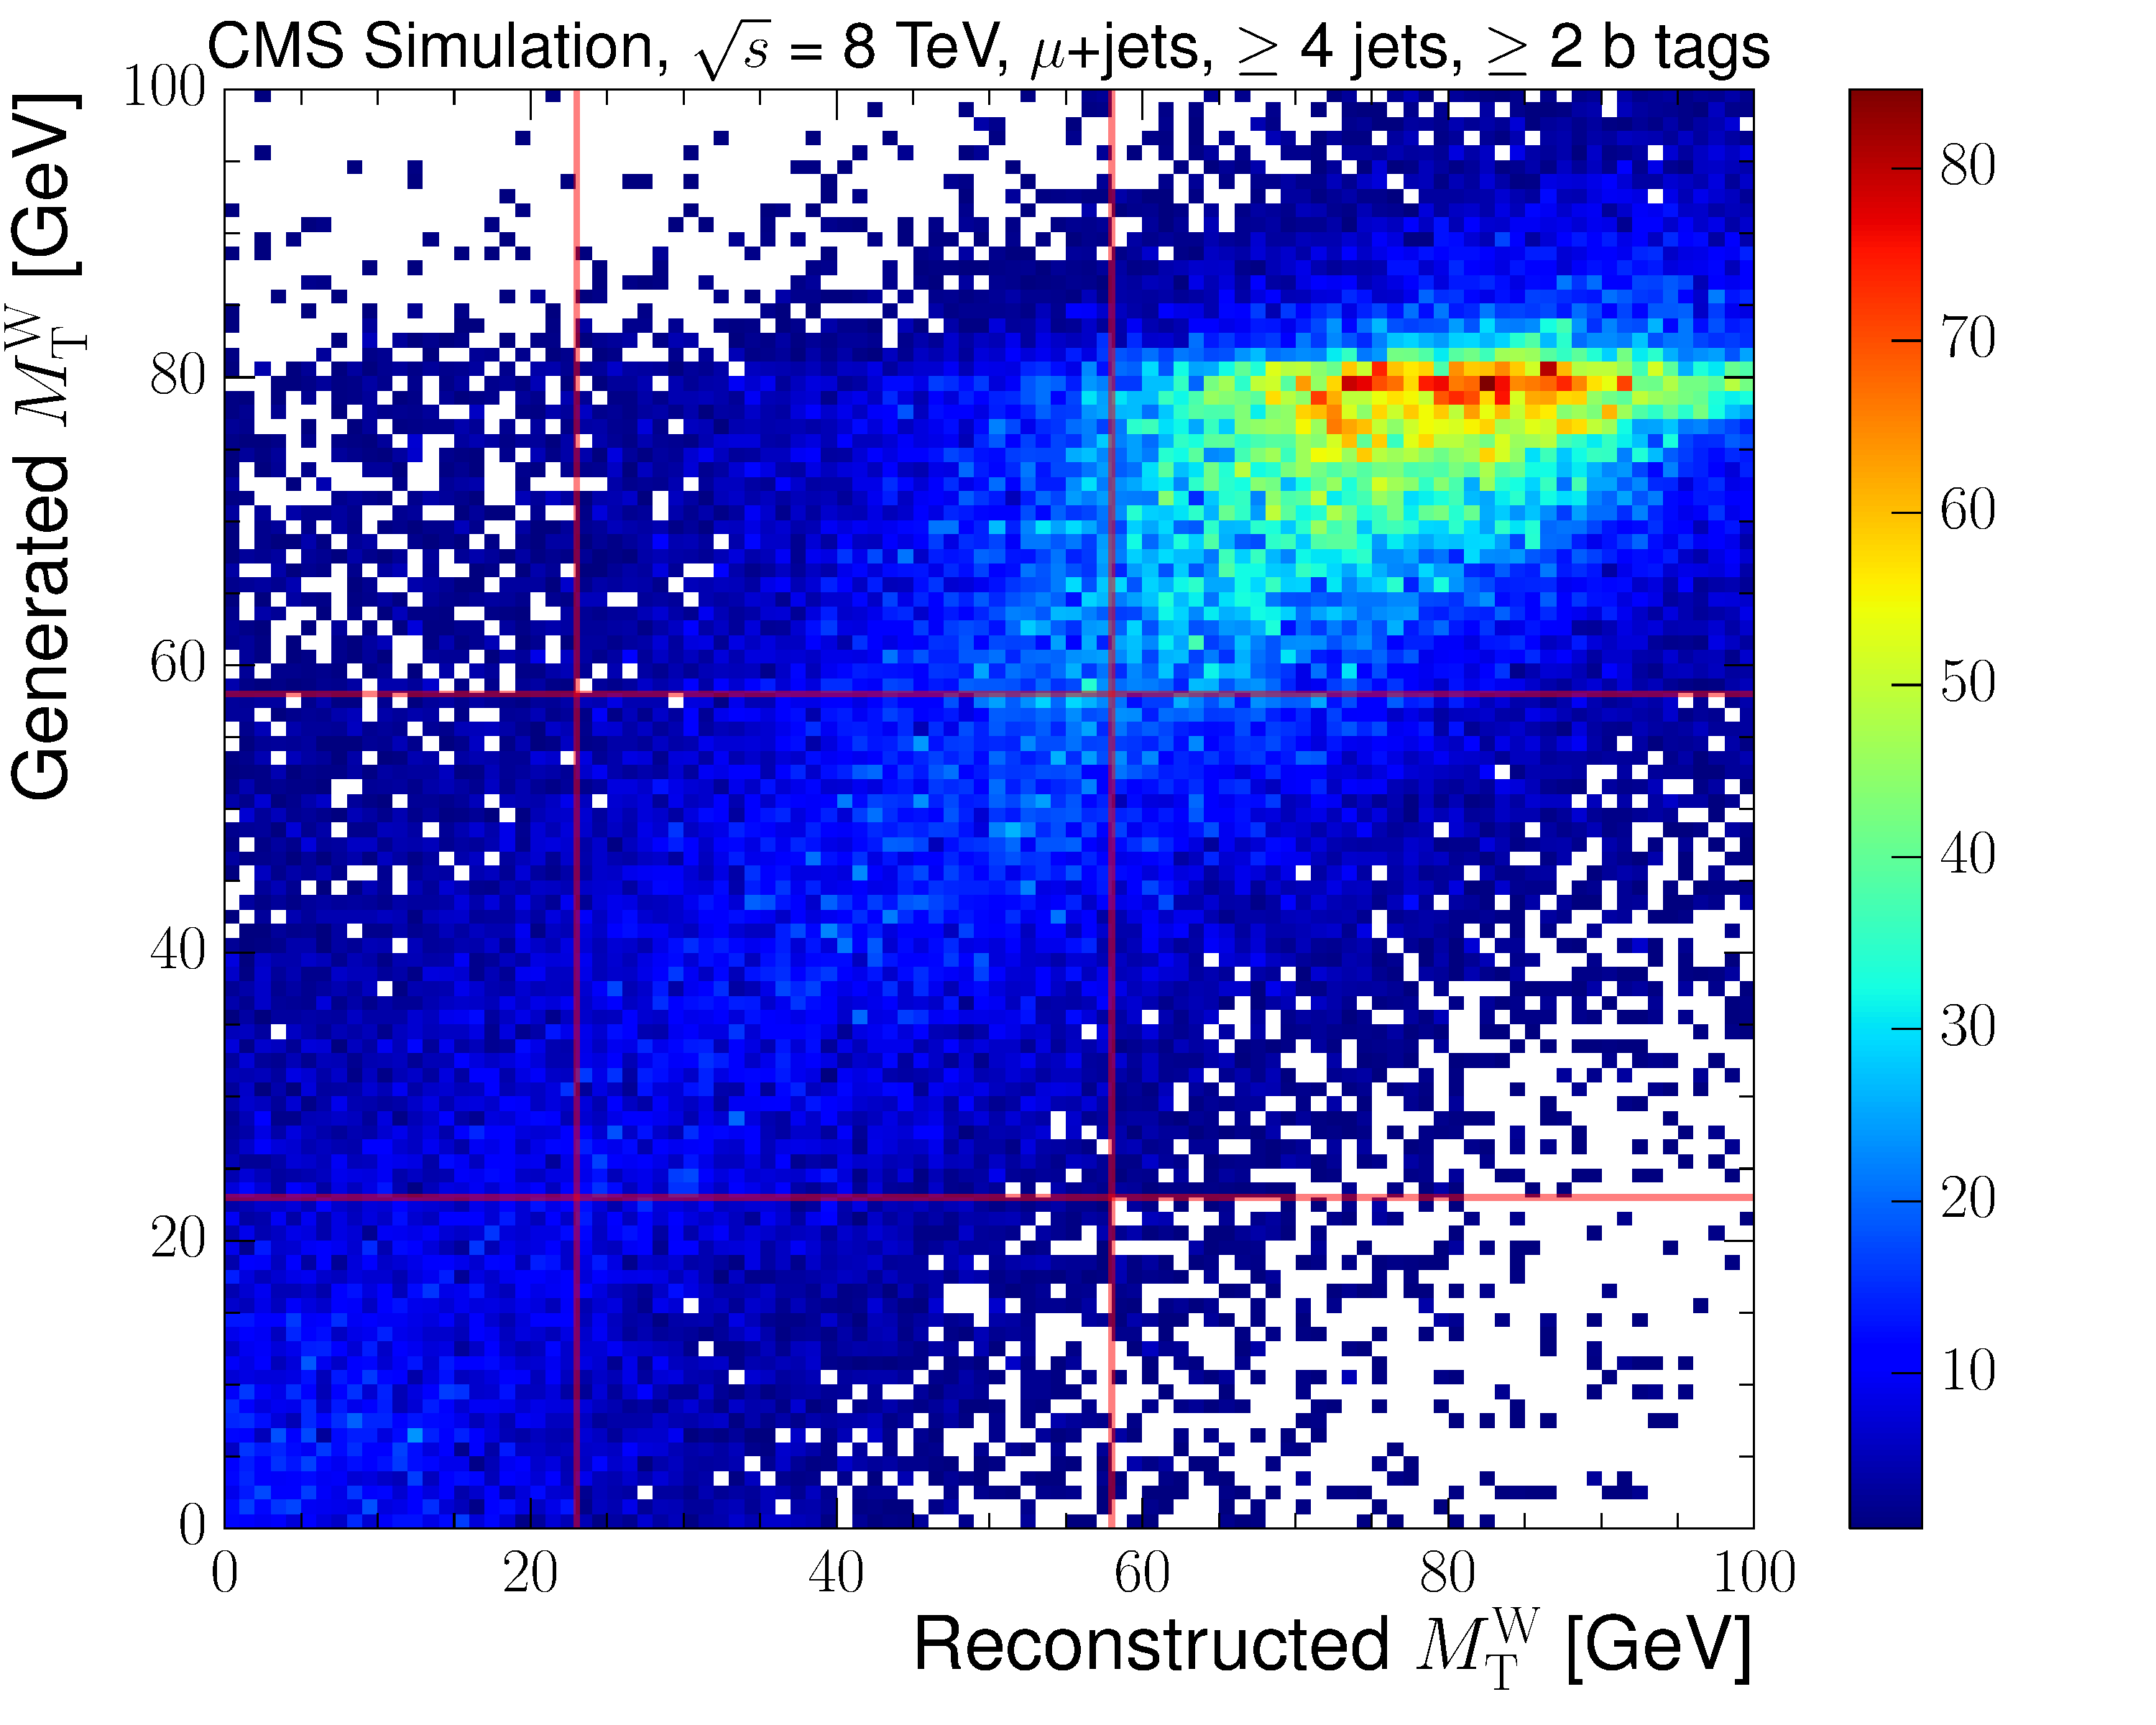
\includegraphics[width=0.48\textwidth]{Chapters/04_Analysis/04b_XSections/images/binning/muon_MT_8TeV.pdf}\\
	 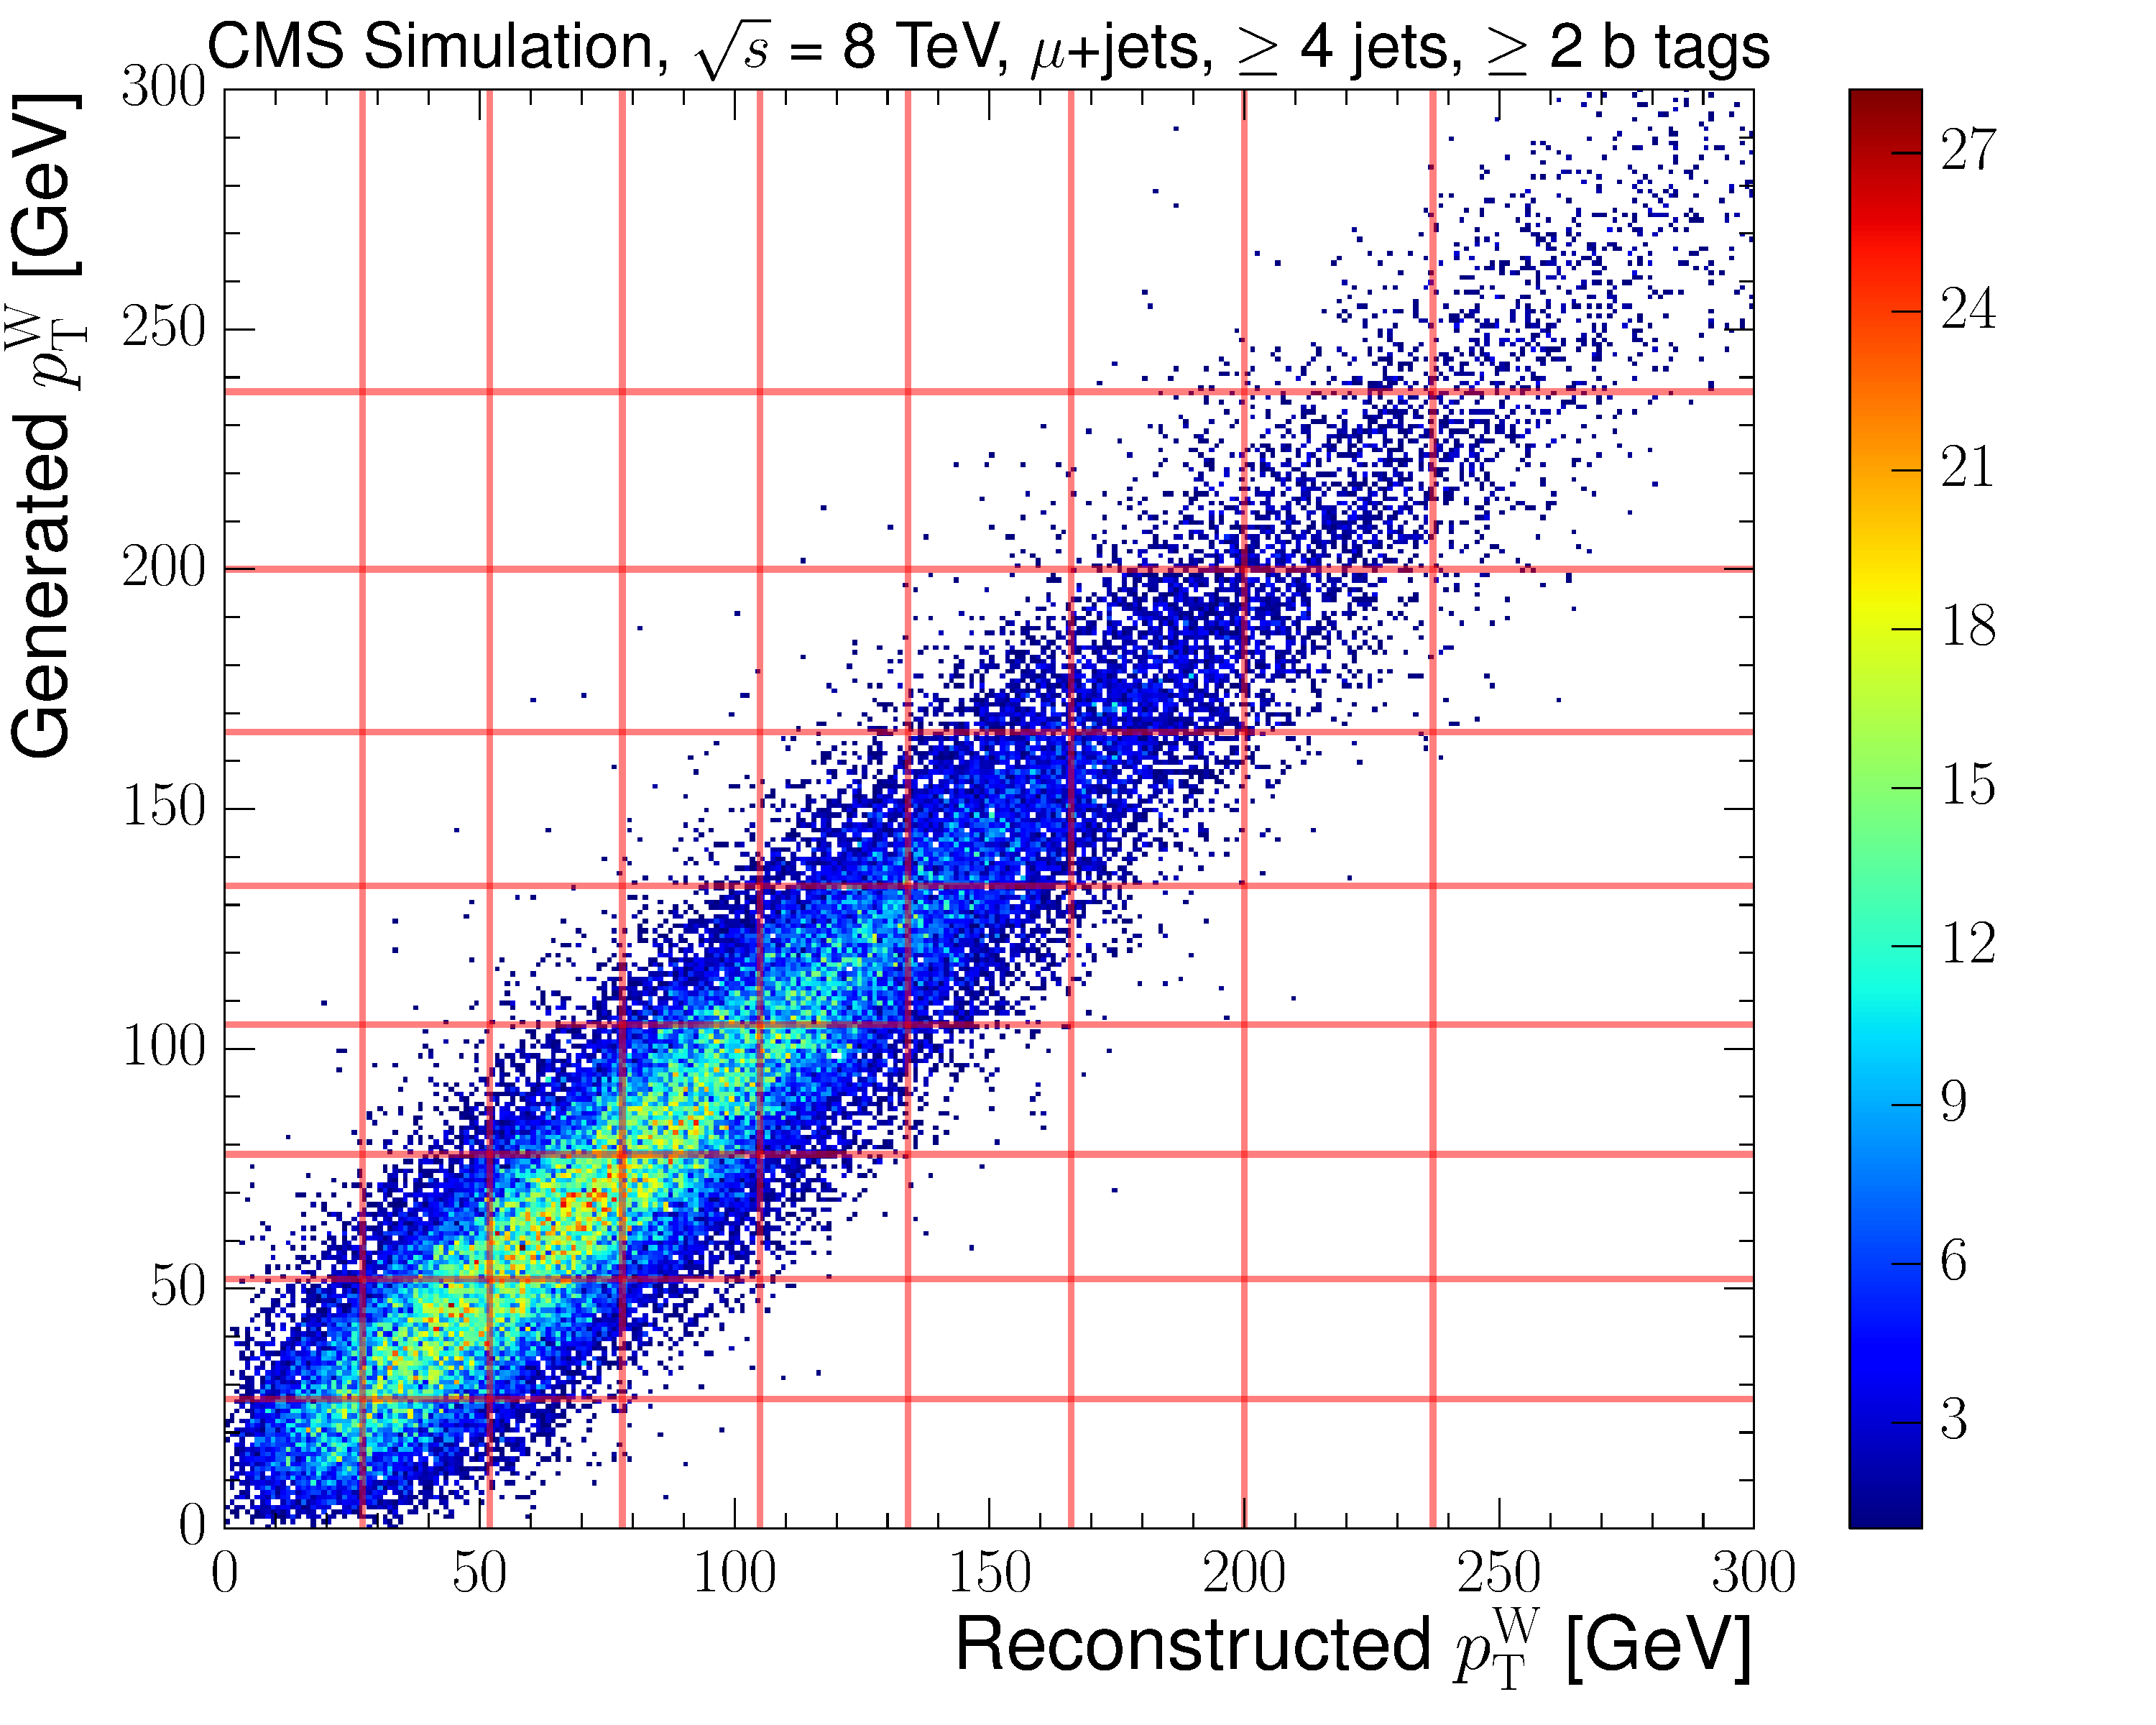
\includegraphics[width=0.48\textwidth]{Chapters/04_Analysis/04b_XSections/images/binning/muon_WPT_8TeV.pdf}\hfill
	 \caption{Generated versus reconstructed distributions of the primary variables \met (upper left), \HT (upper
	 right), \st (middle left), \mt (middle right) and \wpt (lower) with horizontal and vertical lines
	 representing the boundaries of the selected bins at $\sqrt{s}=8\TeV$ in the muon+jets channel. These
	 distributions are obtained using \ttbar Monte Carlo simulation.}
     \label{fig:binning_7TeV_muon}
 \end{figure}

 \begin{figure}[hbtp]
    \centering
     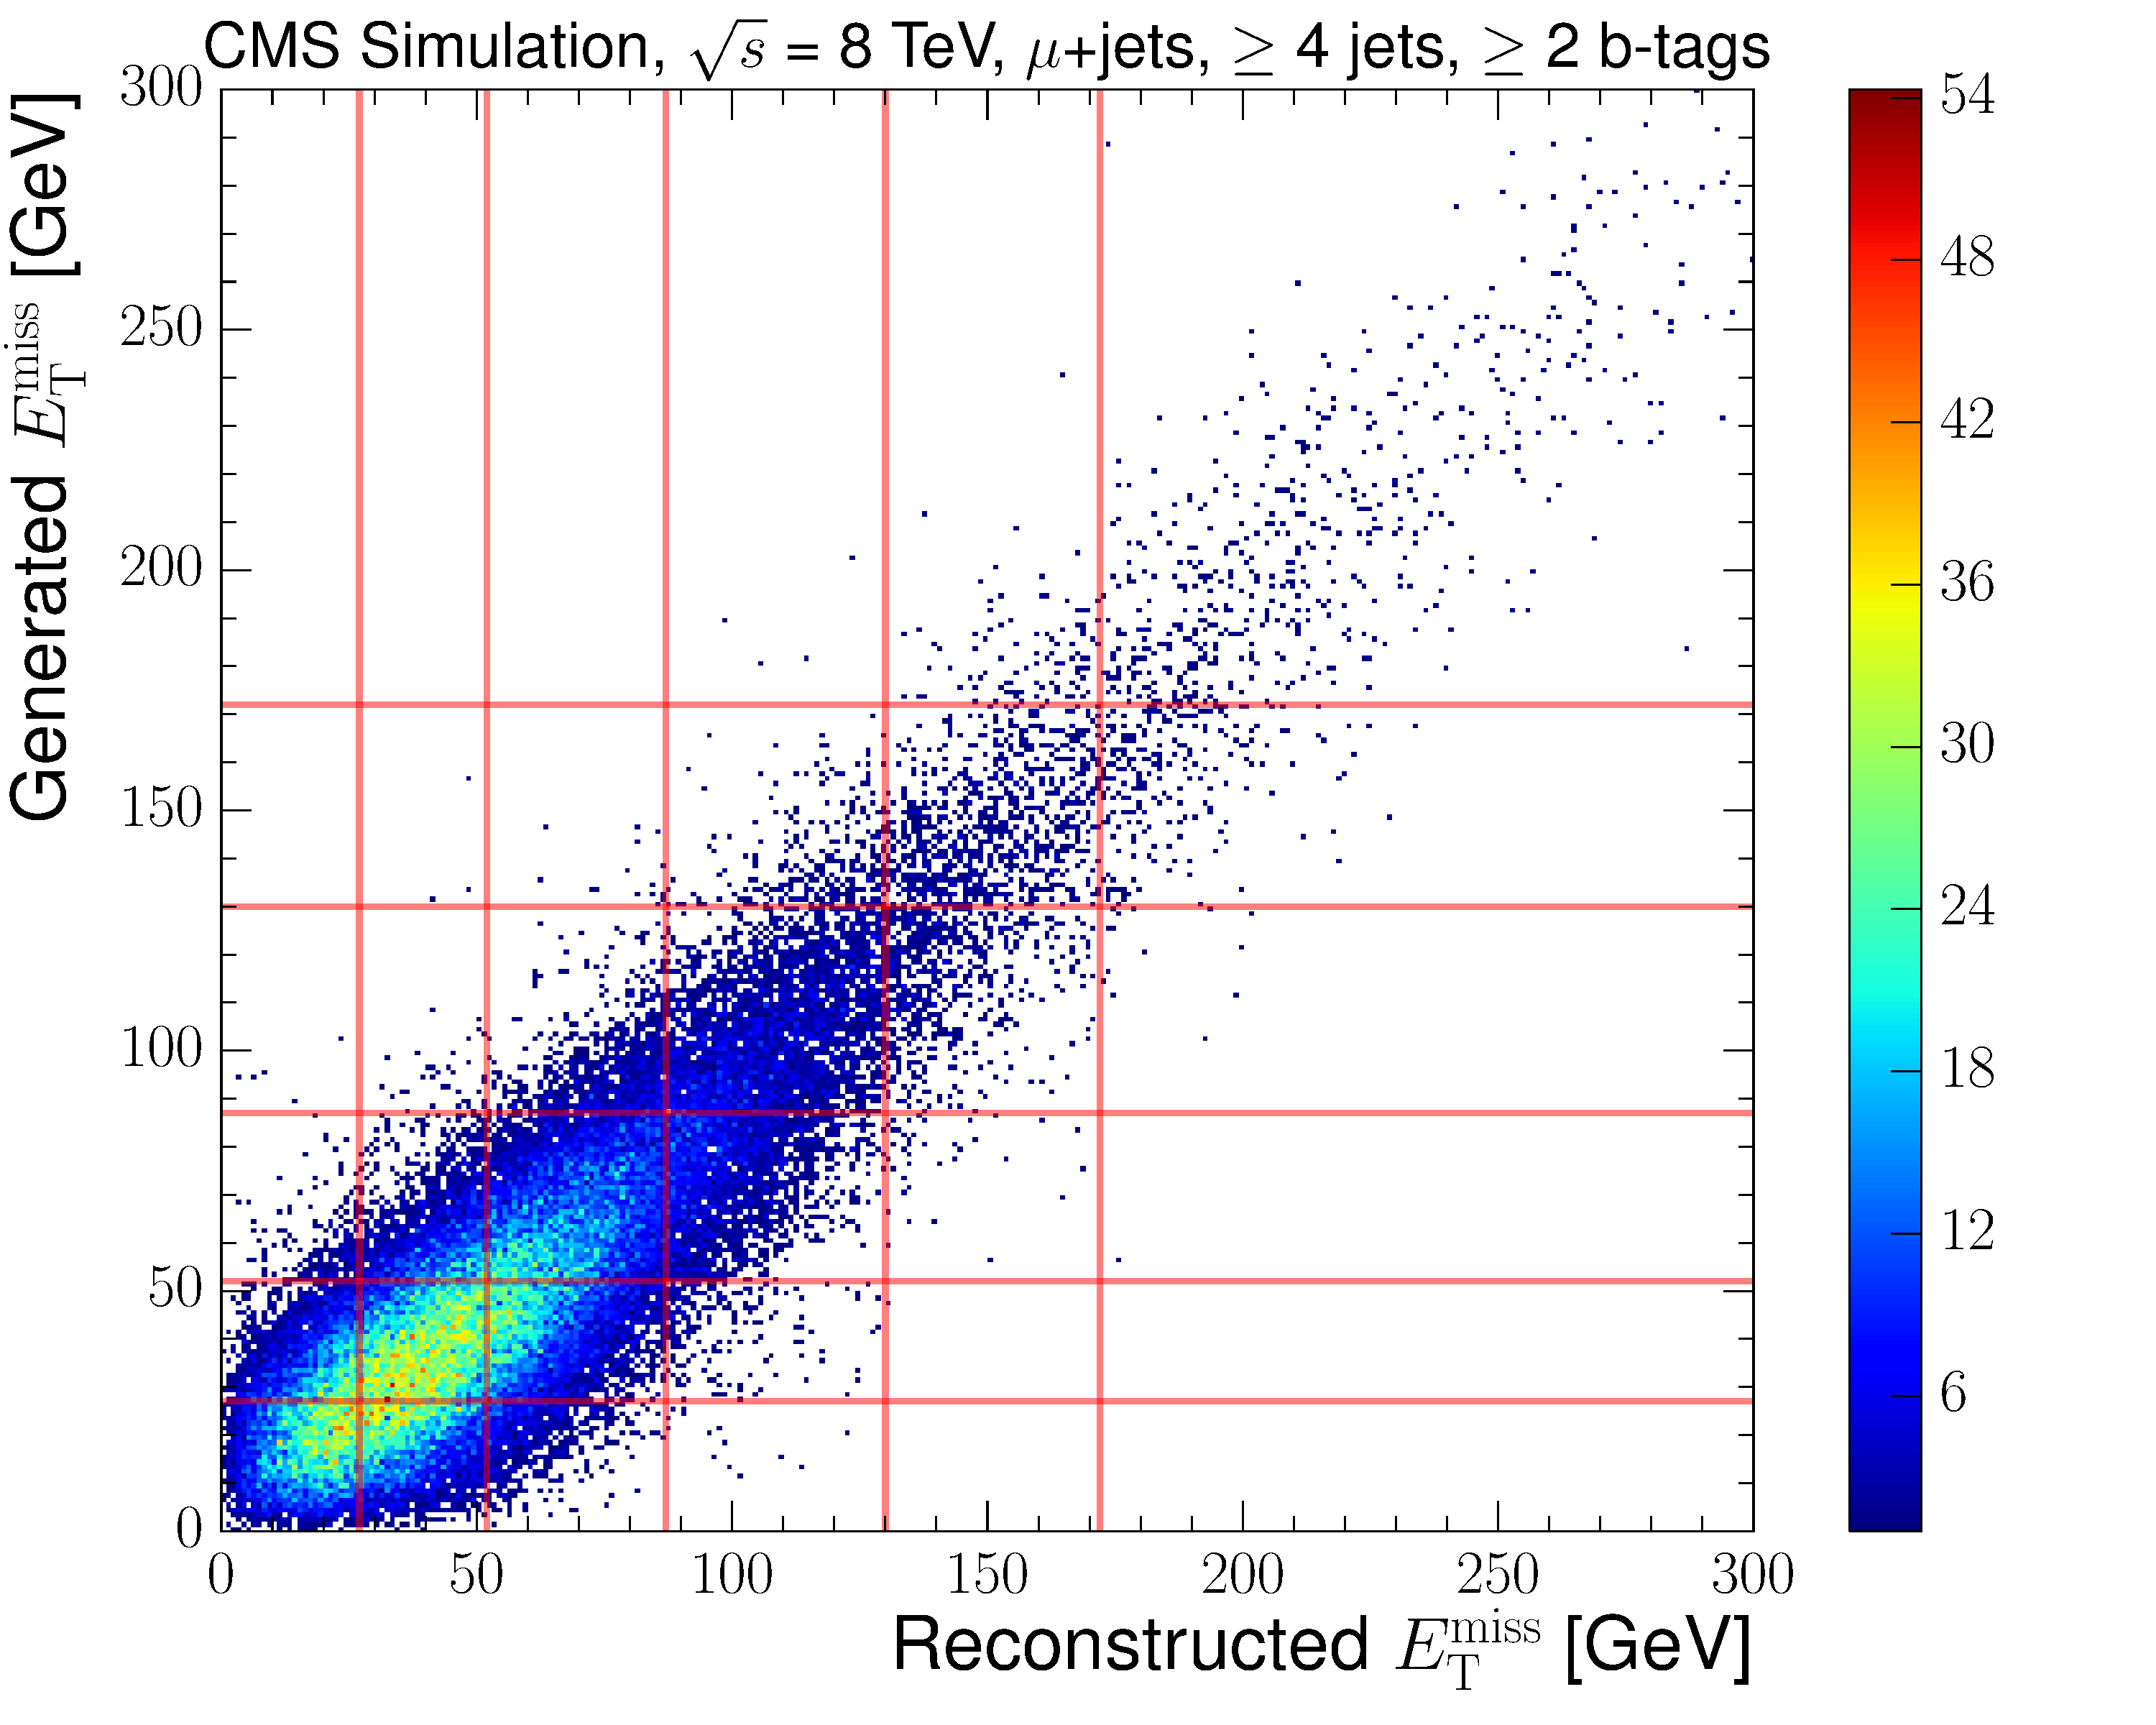
\includegraphics[width=0.48\textwidth]{Chapters/04_Analysis/04b_XSections/images/binning/muon_MET_8TeV.pdf}\hfill
     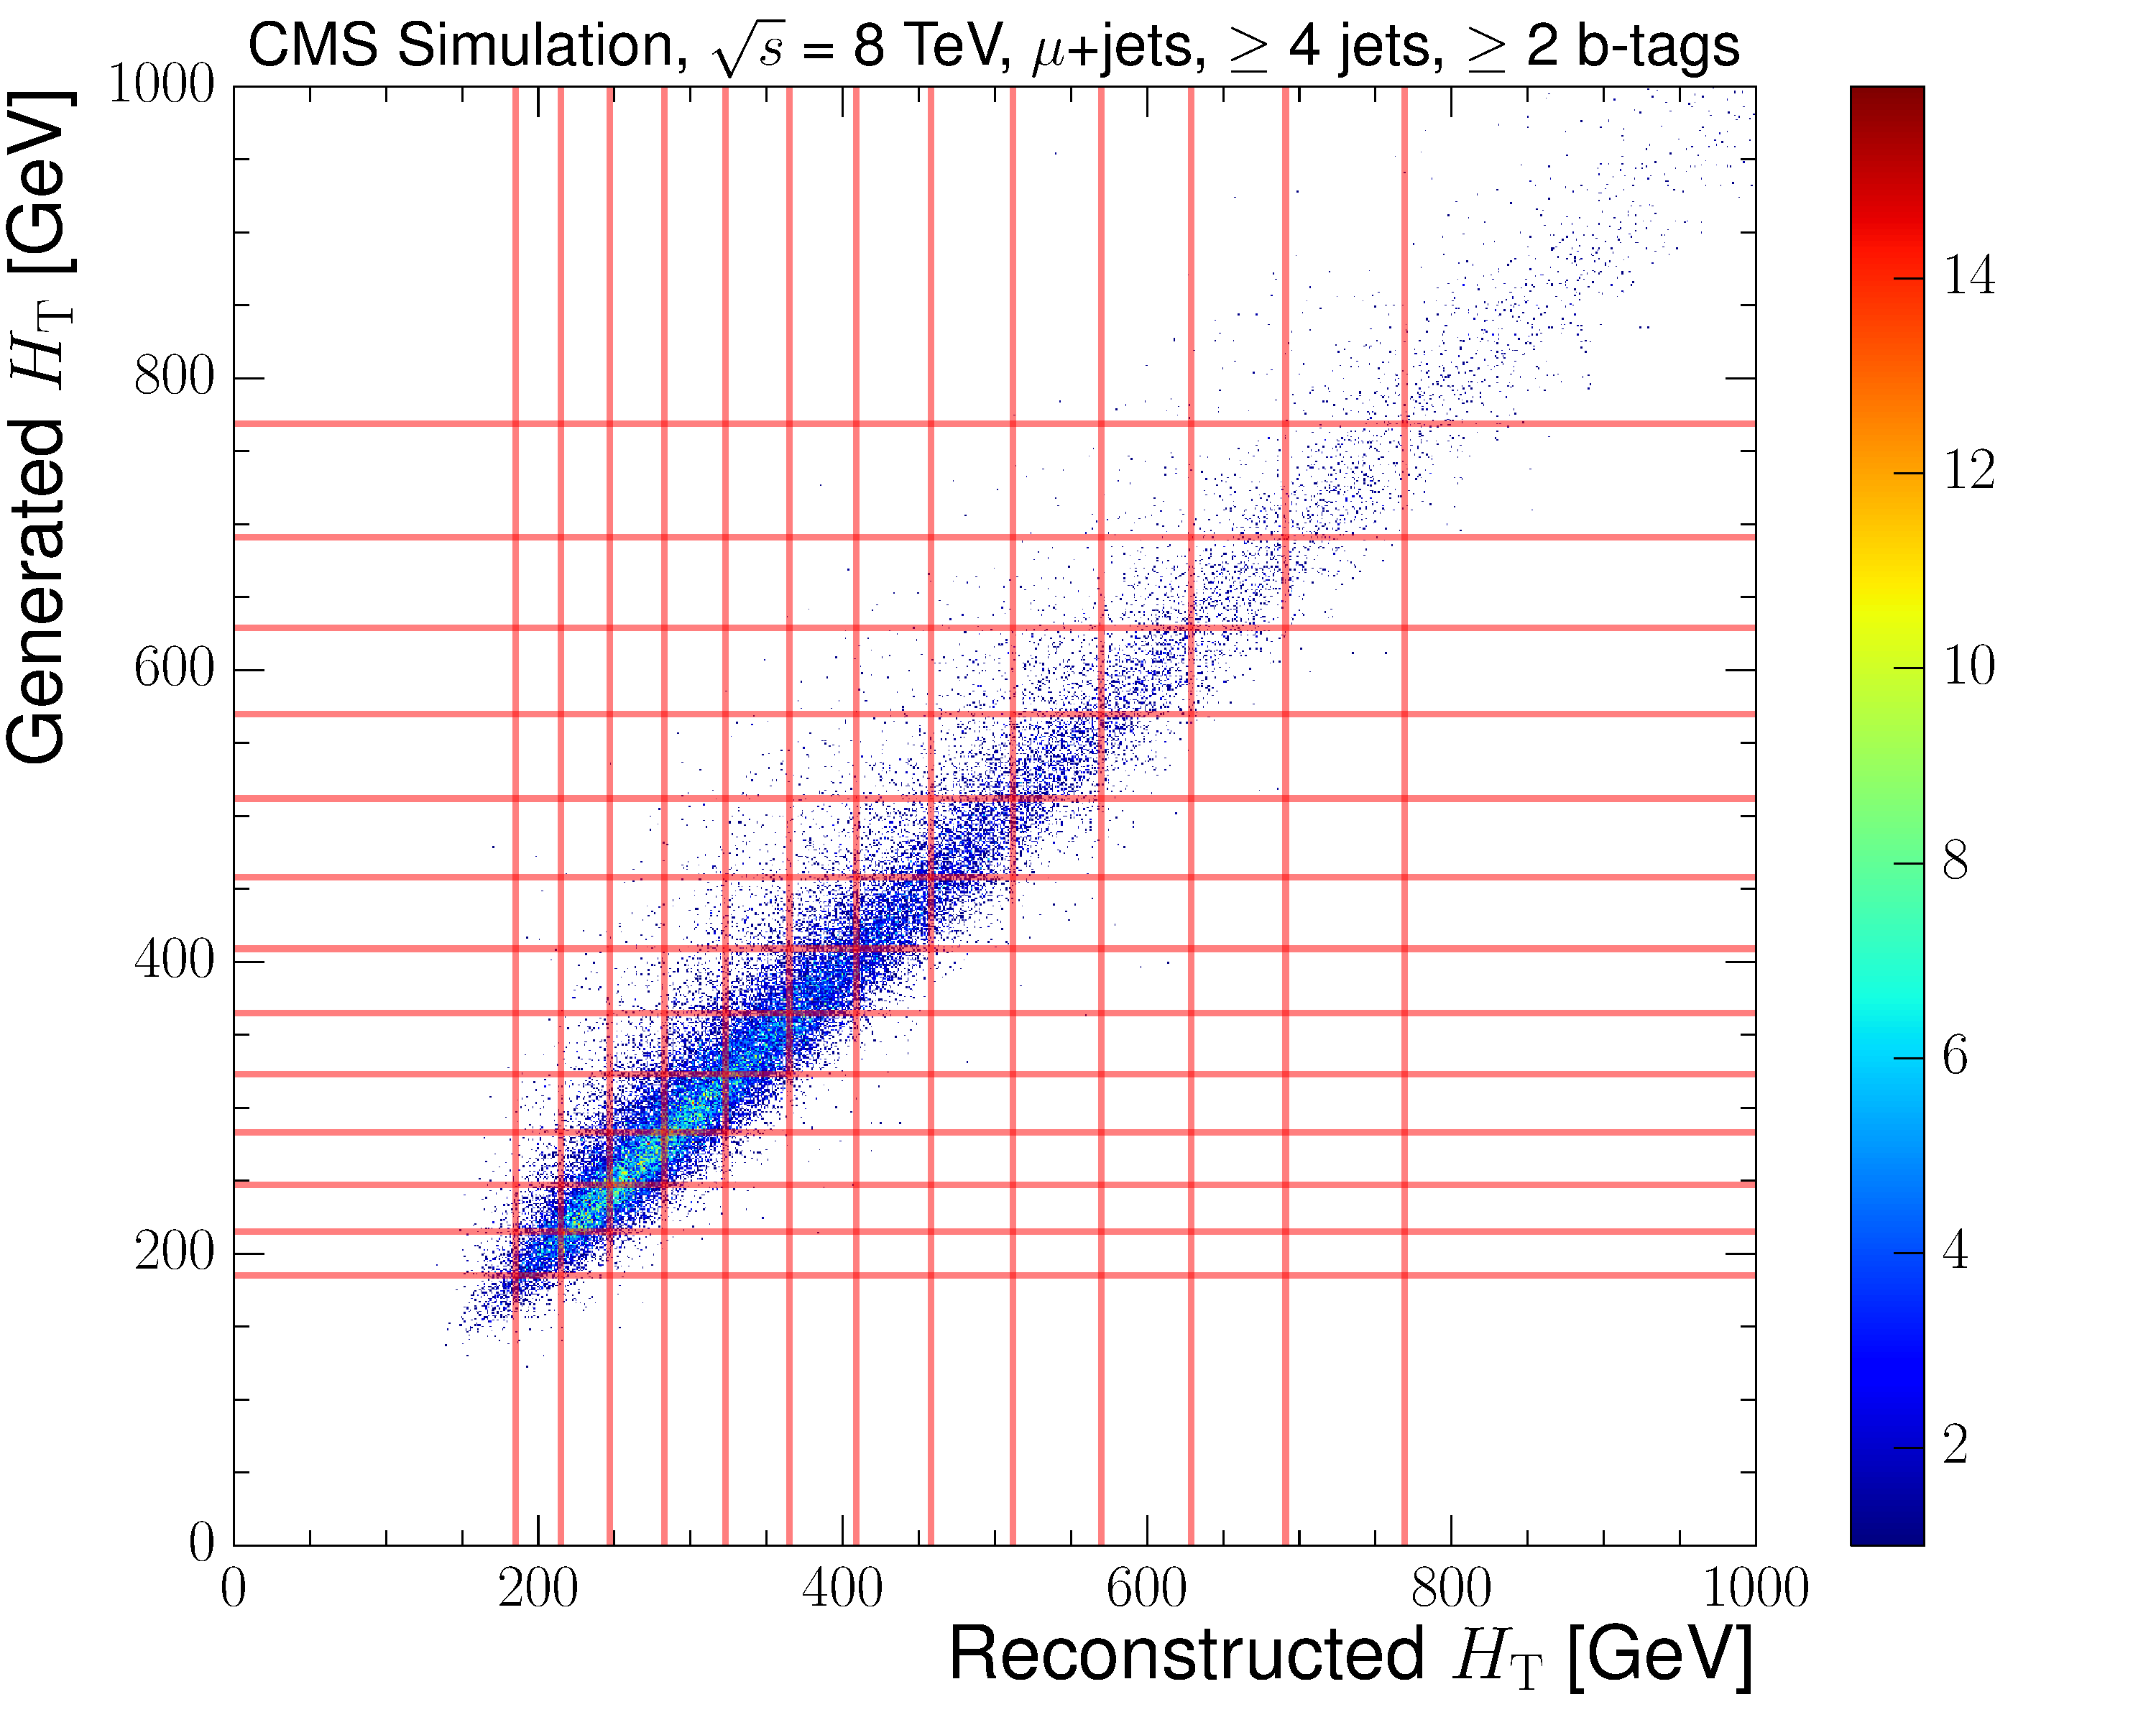
\includegraphics[width=0.48\textwidth]{Chapters/04_Analysis/04b_XSections/images/binning/muon_HT_8TeV.pdf}\\
     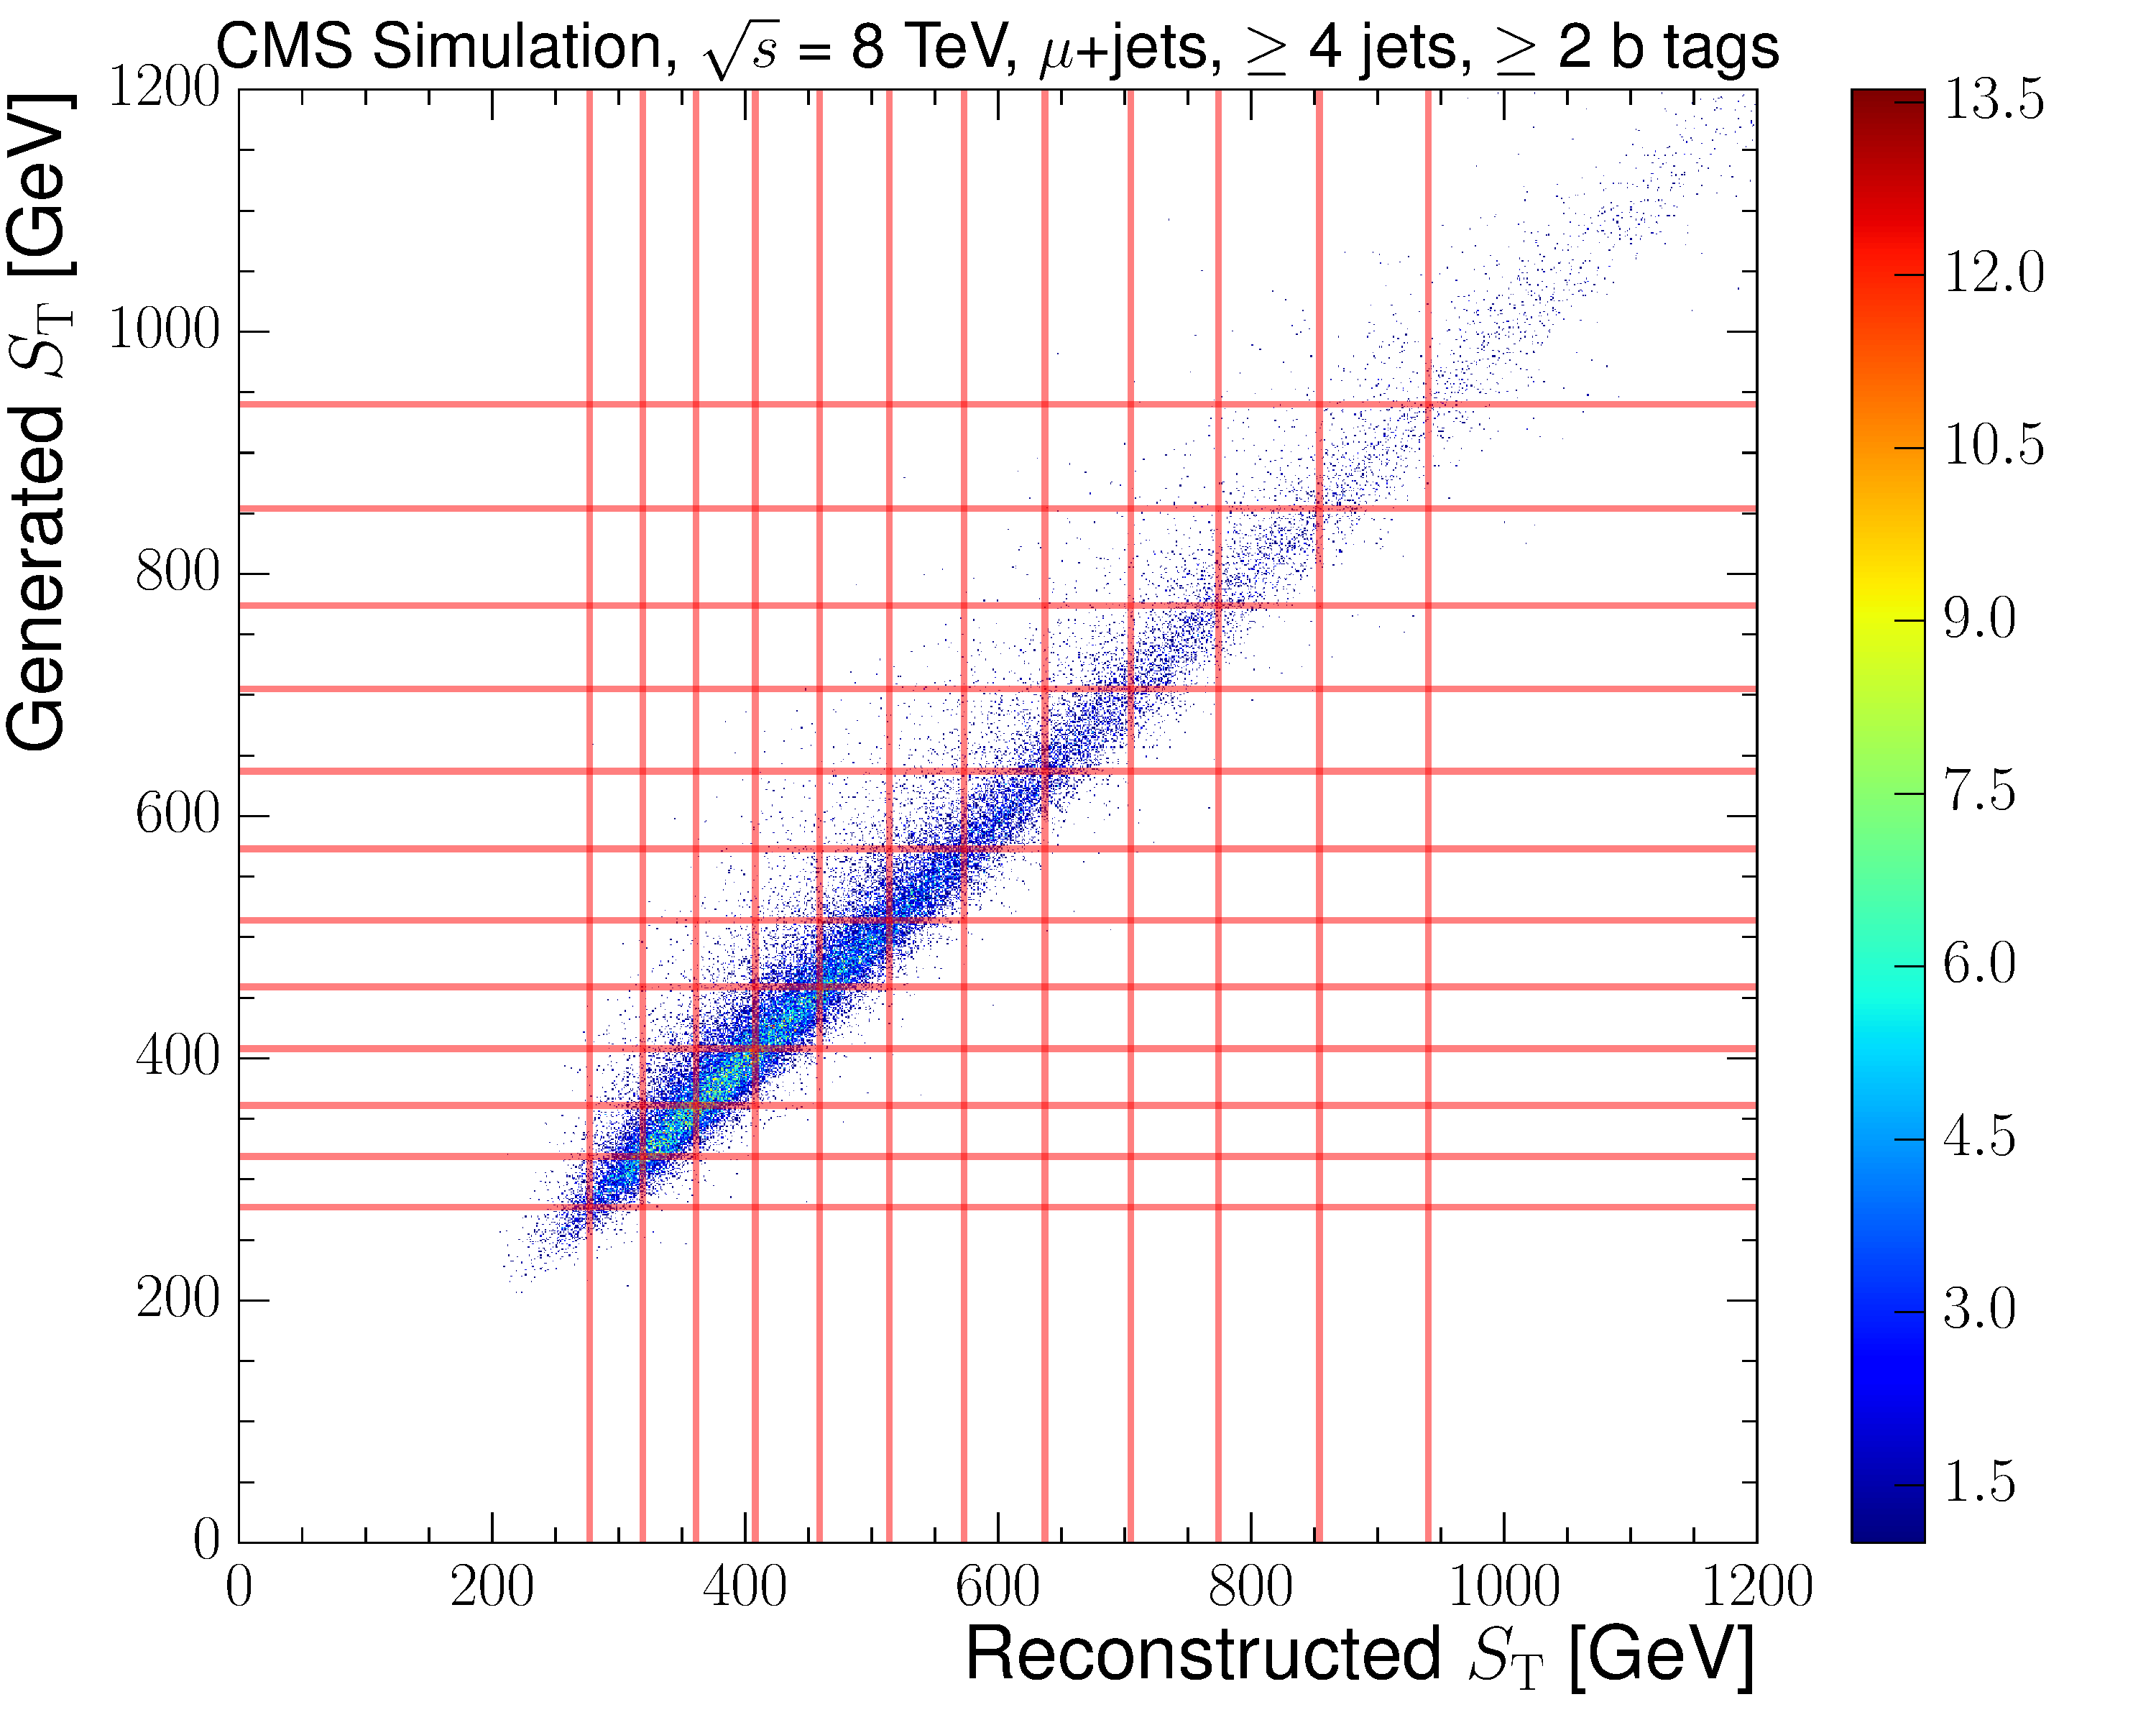
\includegraphics[width=0.48\textwidth]{Chapters/04_Analysis/04b_XSections/images/binning/muon_ST_8TeV.pdf}\hfill
     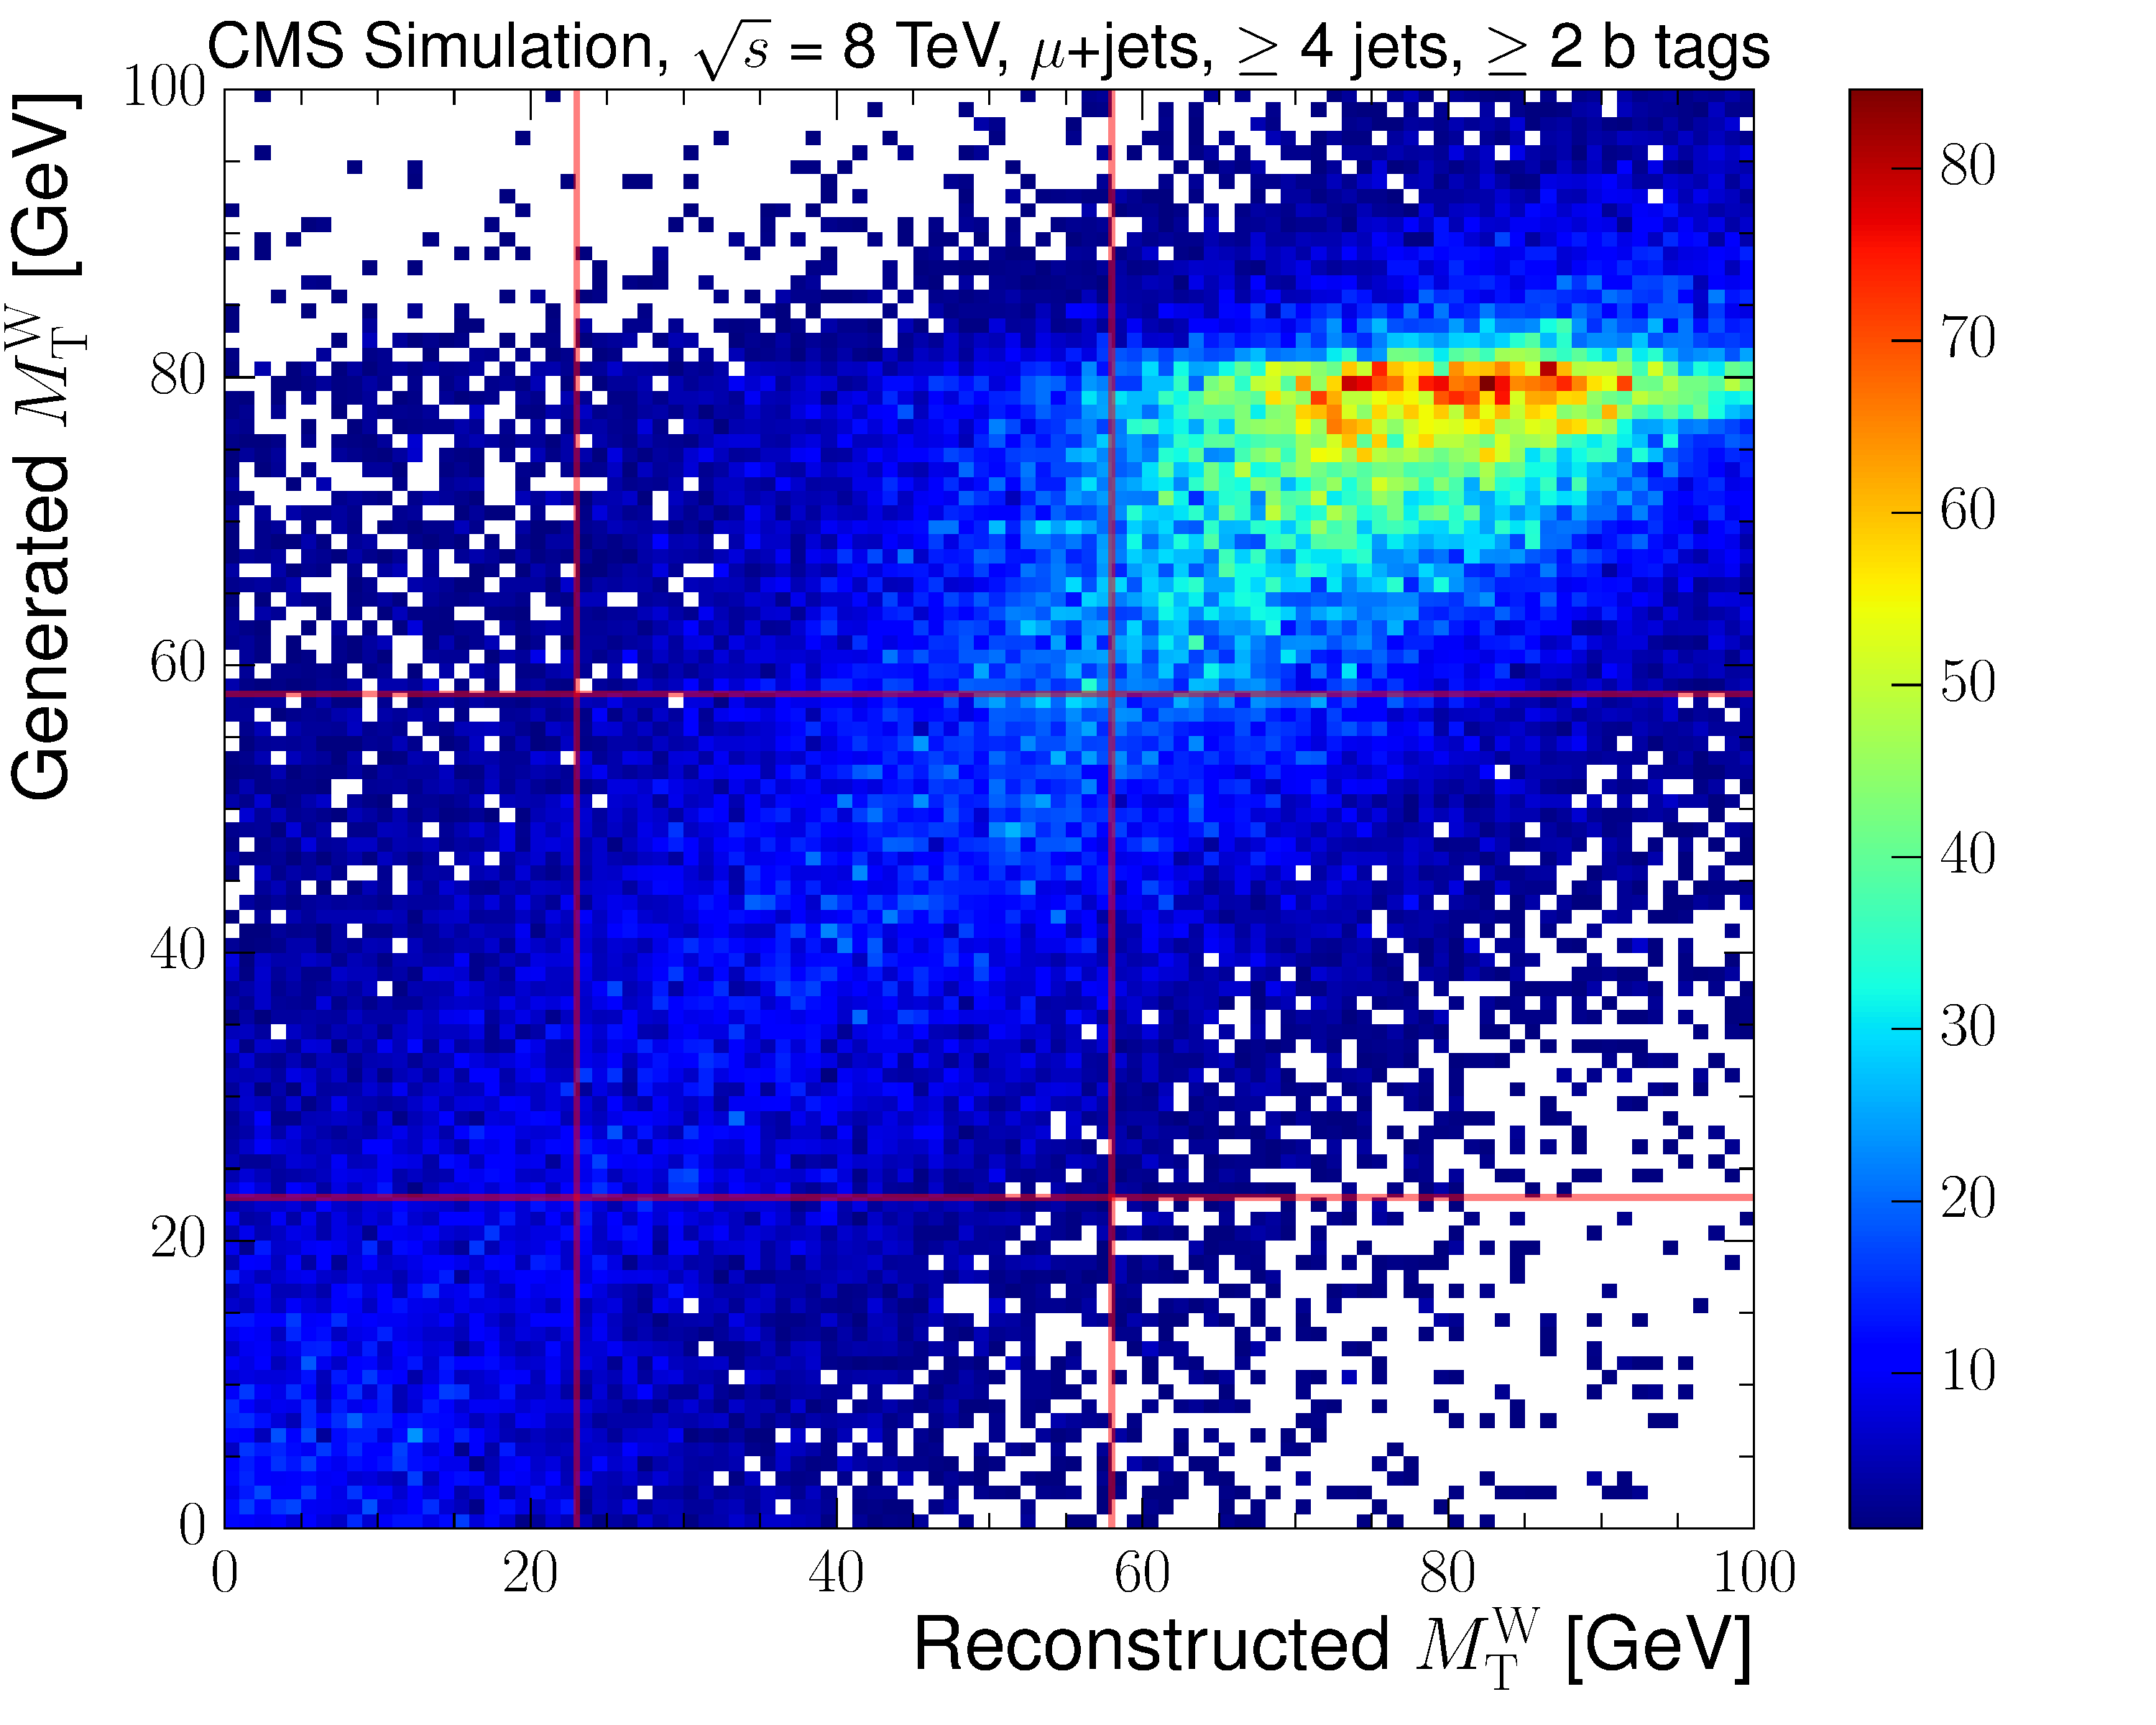
\includegraphics[width=0.48\textwidth]{Chapters/04_Analysis/04b_XSections/images/binning/muon_MT_8TeV.pdf}\\
	 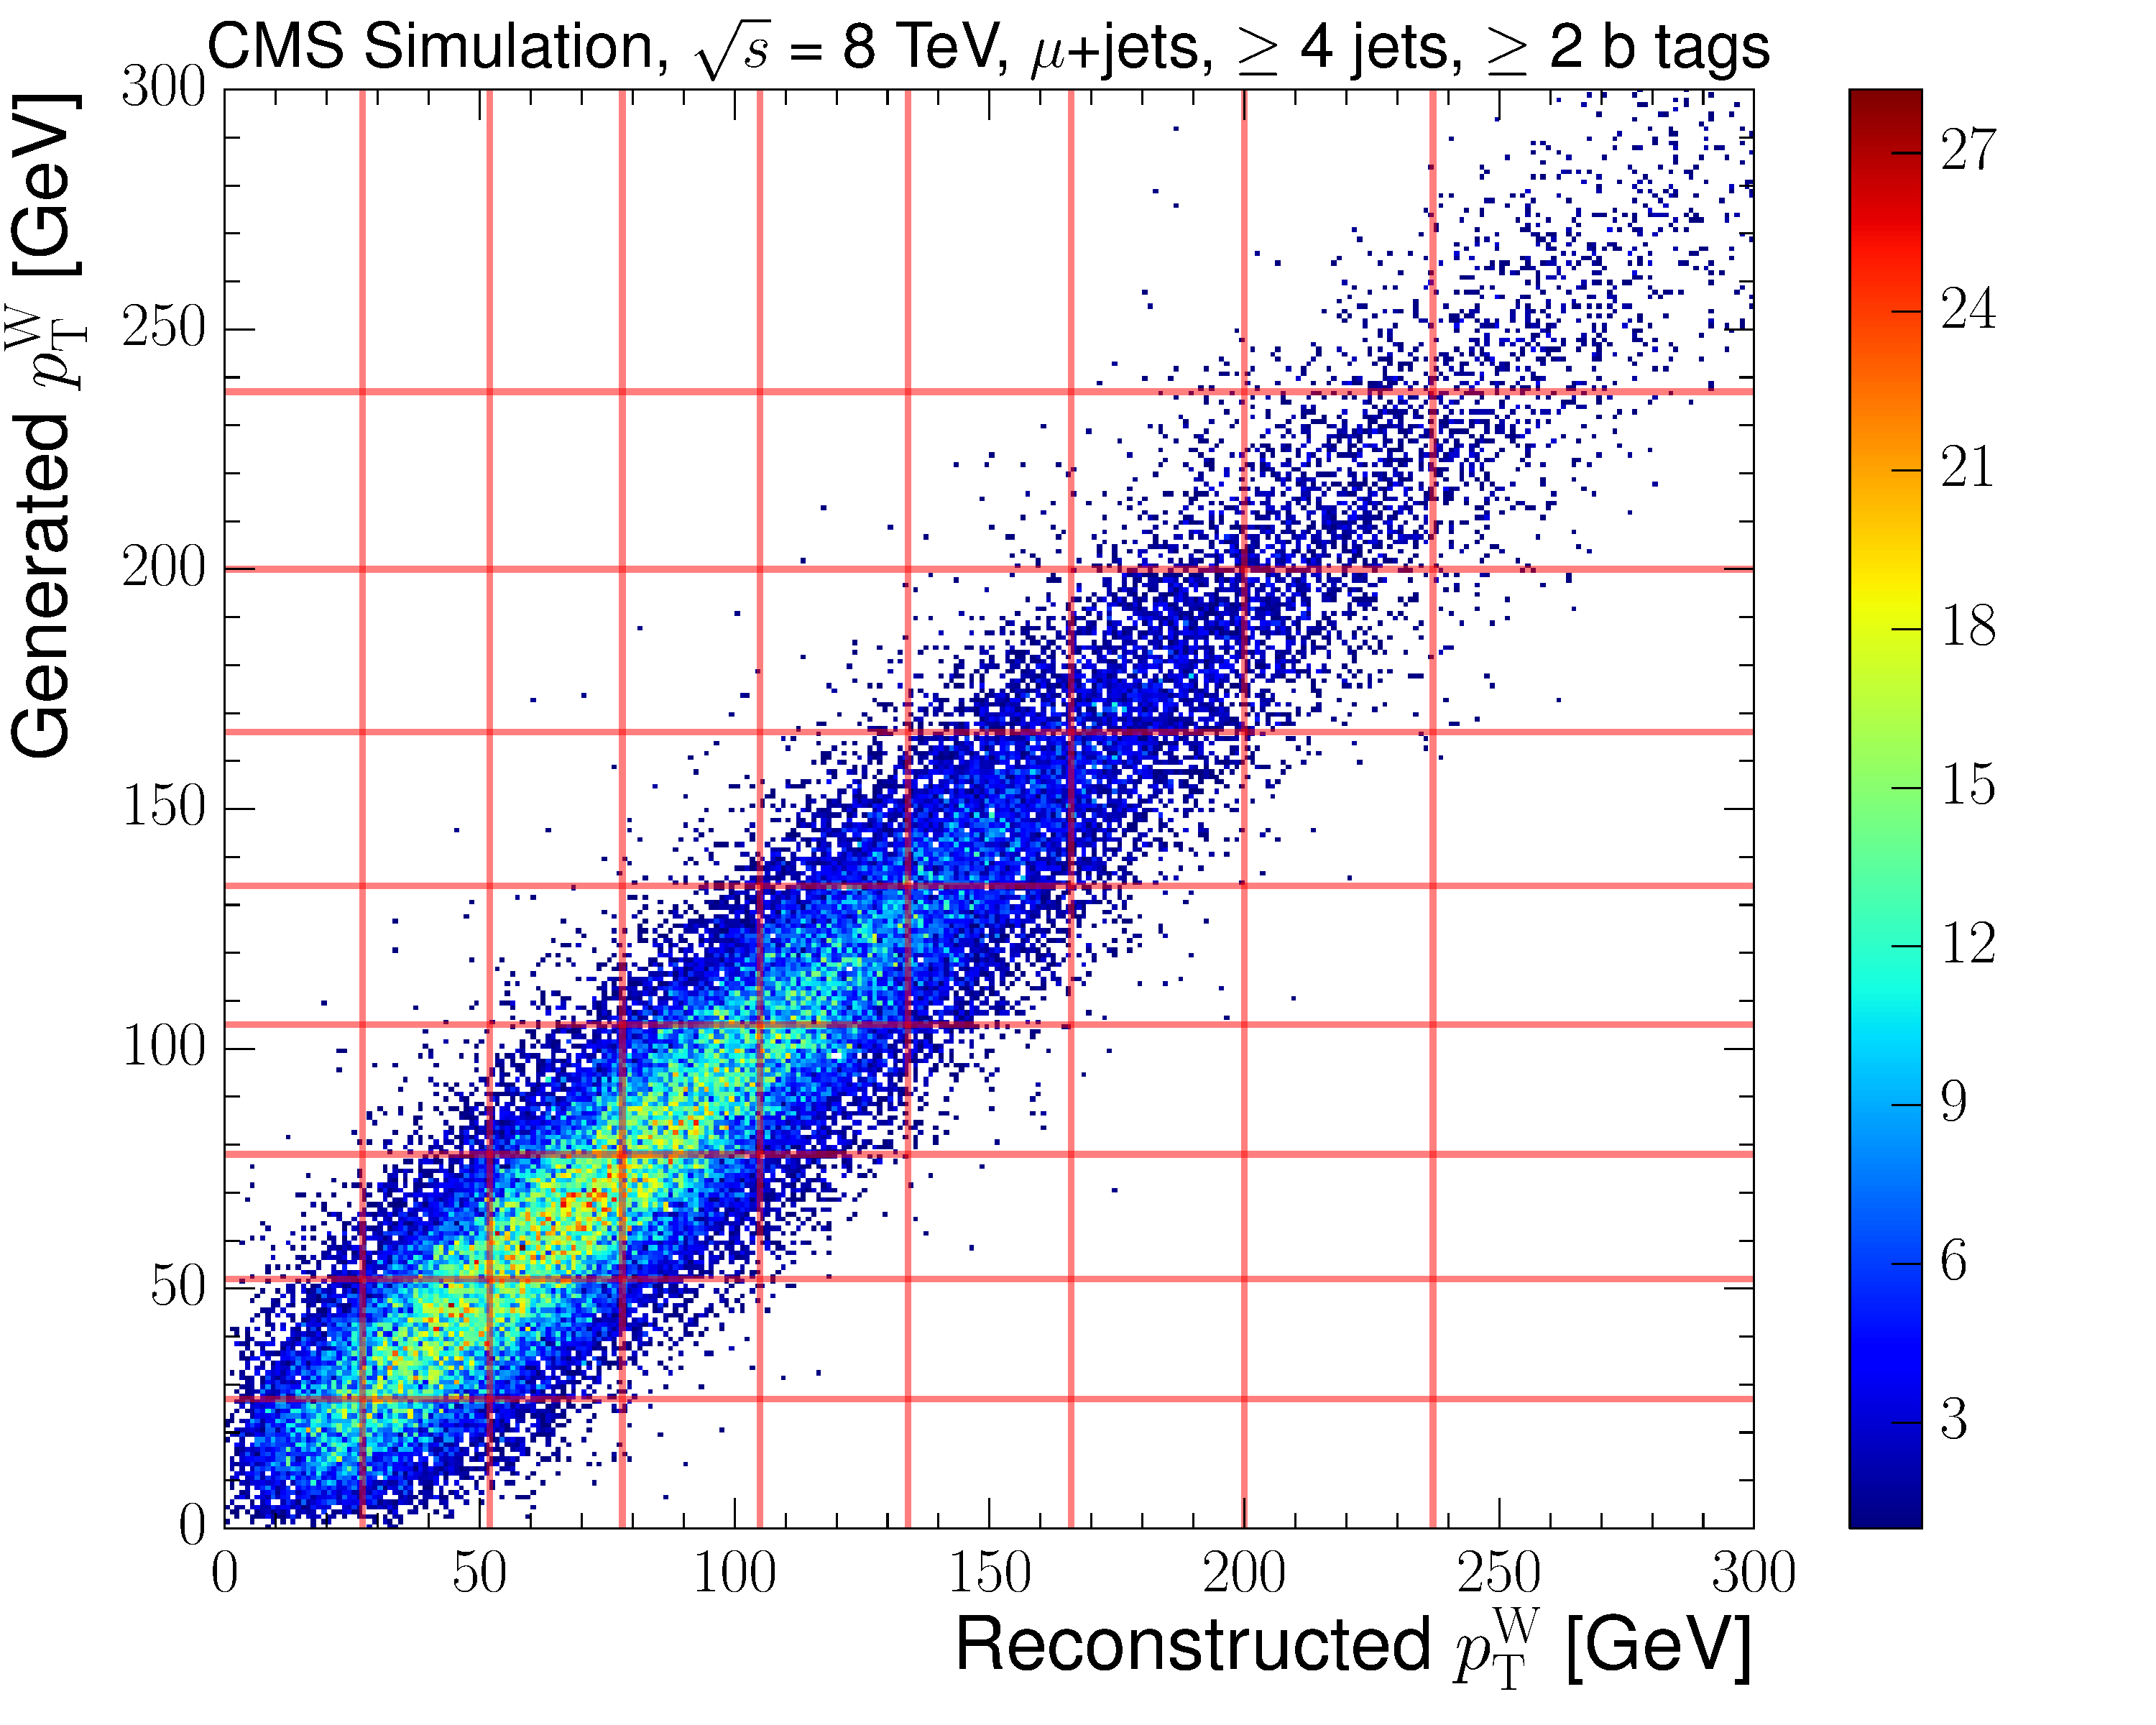
\includegraphics[width=0.48\textwidth]{Chapters/04_Analysis/04b_XSections/images/binning/muon_WPT_8TeV.pdf}\hfill
	 \caption{Generated versus reconstructed distributions of the primary variables \met (upper left), \HT (upper
	 right), \st (middle left), \mt (middle right) and \wpt (lower) with horizontal and vertical lines
	 representing the boundaries of the selected bins at $\sqrt{s}=8\TeV$ in the muon+jets channel. These
	 distributions are obtained using \ttbar Monte Carlo simulation.}
     \label{fig:binning_8TeV_muon}
 \end{figure}
 
\clearpage

~\section*{Binning choice tables}
\label{as:binning_tables_electron}

\begin{table}[ht]
\centering
\resizebox*{!}{\textheight} {
\begin{tabular}{lrrr}
\hline
\met bin (\GeV) &  purity & stability & number of events\\
\hline
0 - 27 & 0.649 & 0.533 & 1367\\
27 - 52 & 0.588 & 0.538 & 2187\\
52 - 87 & 0.537 & 0.636 & 1691\\
87 - 130 & 0.542 & 0.666 & 660\\
130 - 172 & 0.521 & 0.624 & 179\\
$\geq 172$ & 0.711 & 0.824 & 119\\
\hline
\HT bin (\GeV) &  purity & stability & number of events\\
\hline
0 - 186 & 0.589 & 0.567 & 102\\
186 - 216 & 0.546 & 0.565 & 344\\
216 - 249 & 0.542 & 0.585 & 676\\
249 - 286 & 0.541 & 0.575 & 884\\
286 - 326 & 0.543 & 0.556 & 896\\
326 - 368 & 0.536 & 0.538 & 765\\
368 - 412 & 0.537 & 0.517 & 598\\
412 - 462 & 0.566 & 0.538 & 518\\
462 - 516 & 0.573 & 0.531 & 375\\
516 - 574 & 0.580 & 0.537 & 264\\
574 - 634 & 0.590 & 0.529 & 172\\
634 - 696 & 0.581 & 0.539 & 113\\
696 - 781 & 0.660 & 0.624 & 100\\
$\geq 781$ & 0.886 & 0.814 & 117\\
\hline
\st bin (\GeV) &  purity & stability & number of events\\
\hline
0 - 277 & 0.565 & 0.550 & 108\\
277 - 319 & 0.564 & 0.549 & 422\\
319 - 361 & 0.538 & 0.543 & 743\\
361 - 408 & 0.530 & 0.547 & 939\\
408 - 459 & 0.527 & 0.539 & 897\\
459 - 514 & 0.534 & 0.536 & 764\\
514 - 573 & 0.539 & 0.530 & 601\\
573 - 637 & 0.548 & 0.532 & 449\\
637 - 705 & 0.548 & 0.534 & 305\\
705 - 774 & 0.540 & 0.523 & 194\\
774 - 854 & 0.576 & 0.566 & 151\\
854 - 946 & 0.613 & 0.580 & 102\\
$\geq 946$ & 0.838 & 0.837 & 133\\
\hline
\mt bin (\GeV) &  purity & stability & number of events\\
\hline
0 - 23 & 0.528 & 0.598 & 659\\
23 - 58 & 0.515 & 0.562 & 1557\\
$\geq 58$ & 0.845 & 0.786 & 4518\\
\hline
\wpt bin (\GeV) &  purity & stability & number of events\\
\hline
0 - 27 & 0.597 & 0.549 & 467\\
27 - 52 & 0.551 & 0.526 & 960\\
52 - 78 & 0.550 & 0.540 & 1228\\
78 - 105 & 0.539 & 0.538 & 1107\\
105 - 134 & 0.537 & 0.554 & 857\\
134 - 166 & 0.537 & 0.568 & 570\\
166 - 200 & 0.524 & 0.564 & 314\\
200 - 237 & 0.536 & 0.573 & 177\\
$\geq 237$ & 0.707 & 0.789 & 145\\
\hline
\end{tabular}
}
\caption{The selected bins for the measurement in the electron channel at a centre-of-mass energy of 7\TeV. In addition
to the bin ranges the purity, stability and number of expected \ttbar events are shown.}
\label{tab:binning_electron_7TeV}
\end{table}

\begin{table}[ht]
\centering
\begin{tabular}{lrrr}
\hline

\met bin (\GeV) &  purity & stability & number of events\\
\hline
0 - 27 & 0.641 & 0.533 & 1445\\
27 - 52 & 0.587 & 0.536 & 2374\\
52 - 87 & 0.552 & 0.638 & 1982\\
87 - 130 & 0.550 & 0.673 & 770\\
130 - 172 & 0.533 & 0.634 & 207\\
$\geq 172$ & 0.706 & 0.844 & 133\\
\hline
\HT bin (\GeV) &  purity & stability & number of events\\
\hline
0 - 186 & 0.595 & 0.568 & 121\\
186 - 216 & 0.543 & 0.563 & 397\\
216 - 249 & 0.545 & 0.583 & 787\\
249 - 286 & 0.541 & 0.576 & 1008\\
286 - 326 & 0.546 & 0.559 & 1010\\
326 - 368 & 0.540 & 0.538 & 841\\
368 - 412 & 0.547 & 0.529 & 675\\
412 - 462 & 0.569 & 0.542 & 558\\
462 - 516 & 0.584 & 0.537 & 406\\
516 - 574 & 0.585 & 0.547 & 281\\
574 - 634 & 0.590 & 0.542 & 181\\
634 - 696 & 0.597 & 0.546 & 119\\
696 - 781 & 0.682 & 0.623 & 105\\
$\geq 781$ & 0.885 & 0.818 & 117\\
\hline
\st bin (\GeV) &  purity & stability & number of events\\
\hline
0 - 277 & 0.562 & 0.552 & 135\\
277 - 319 & 0.560 & 0.542 & 503\\
319 - 361 & 0.536 & 0.546 & 866\\
361 - 408 & 0.532 & 0.546 & 1056\\
408 - 459 & 0.530 & 0.543 & 1003\\
459 - 514 & 0.538 & 0.540 & 853\\
514 - 573 & 0.543 & 0.531 & 645\\
573 - 637 & 0.553 & 0.534 & 477\\
637 - 705 & 0.548 & 0.539 & 326\\
705 - 774 & 0.542 & 0.523 & 200\\
774 - 854 & 0.571 & 0.557 & 152\\
854 - 946 & 0.598 & 0.585 & 101\\
$\geq 946$ & 0.847 & 0.832 & 138\\
\hline
\mt bin (\GeV) &  purity & stability & number of events\\
\hline
0 - 23 & 0.535 & 0.608 & 742\\
23 - 58 & 0.523 & 0.574 & 1777\\
$\geq 58$ & 0.851 & 0.789 & 5093\\
\hline
\wpt bin (\GeV) &  purity & stability & number of events\\
\hline
0 - 27 & 0.599 & 0.544 & 558\\
27 - 52 & 0.559 & 0.529 & 1141\\
52 - 78 & 0.549 & 0.539 & 1369\\
78 - 105 & 0.531 & 0.538 & 1190\\
105 - 134 & 0.537 & 0.557 & 928\\
134 - 166 & 0.537 & 0.569 & 610\\
166 - 200 & 0.526 & 0.568 & 336\\
200 - 237 & 0.532 & 0.575 & 183\\
$\geq 237$ & 0.689 & 0.794 & 150\\
\hline
\end{tabular}
\caption{The selected bins for the measurement in the muon channel at a centre-of-mass energy of 7\TeV. In addition
to the bin ranges the purity, stability and number of expected \ttbar events are shown.}
\label{tab:binning_muon_7TeV}
\end{table}

\begin{table}[ht]
\centering
\resizebox*{!}{\textheight} {
\begin{tabular}{lrrr}
\hline
\met bin (\GeV) &  purity & stability & number of events\\
\hline
0 - 27 & 0.634 & 0.505 & 6400\\
27 - 52 & 0.557 & 0.507 & 9823\\
52 - 87 & 0.503 & 0.606 & 7792\\
87 - 130 & 0.517 & 0.643 & 3239\\
130 - 172 & 0.500 & 0.598 & 904\\
$\geq 172$ & 0.700 & 0.840 & 670\\
\hline
\HT bin (\GeV) &  purity & stability & number of events\\
\hline
0 - 186 & 0.556 & 0.514 & 430\\
186 - 216 & 0.511 & 0.508 & 1408\\
216 - 249 & 0.508 & 0.540 & 2878\\
249 - 286 & 0.511 & 0.540 & 3869\\
286 - 326 & 0.502 & 0.524 & 3892\\
326 - 368 & 0.508 & 0.511 & 3463\\
368 - 412 & 0.506 & 0.500 & 2828\\
412 - 462 & 0.532 & 0.510 & 2457\\
462 - 516 & 0.534 & 0.509 & 1857\\
516 - 574 & 0.547 & 0.500 & 1256\\
574 - 634 & 0.557 & 0.512 & 902\\
634 - 696 & 0.518 & 0.505 & 584\\
696 - 781 & 0.627 & 0.551 & 572\\
$\geq 781$ & 0.872 & 0.815 & 801\\
\hline
\st bin (\GeV) &  purity & stability & number of events\\
\hline
0 - 277 & 0.580 & 0.500 & 463\\
277 - 319 & 0.539 & 0.500 & 1769\\
319 - 361 & 0.509 & 0.515 & 3204\\
361 - 408 & 0.505 & 0.522 & 4126\\
408 - 459 & 0.501 & 0.514 & 4035\\
459 - 514 & 0.504 & 0.510 & 3532\\
514 - 573 & 0.503 & 0.502 & 2780\\
573 - 637 & 0.517 & 0.510 & 2179\\
637 - 705 & 0.517 & 0.504 & 1507\\
705 - 774 & 0.506 & 0.508 & 1039\\
774 - 854 & 0.540 & 0.504 & 769\\
854 - 946 & 0.552 & 0.550 & 551\\
$\geq 946$ & 0.842 & 0.831 & 909\\
\hline
\mt bin (\GeV) &  purity & stability & number of events\\
\hline
0 - 23 & 0.515 & 0.577 & 3245\\
23 - 58 & 0.507 & 0.541 & 7446\\
$\geq 58$ & 0.823 & 0.774 & 20751\\
\hline
\wpt bin (\GeV) &  purity & stability & number of events\\
\hline
0 - 27 & 0.556 & 0.505 & 1962\\
27 - 52 & 0.531 & 0.507 & 4354\\
52 - 78 & 0.527 & 0.513 & 5536\\
78 - 105 & 0.515 & 0.510 & 5131\\
105 - 134 & 0.510 & 0.533 & 4051\\
134 - 166 & 0.518 & 0.546 & 2775\\
166 - 200 & 0.502 & 0.544 & 1590\\
200 - 237 & 0.511 & 0.545 & 903\\
$\geq 237$ & 0.683 & 0.790 & 792\\
\hline
\end{tabular}
}
\caption{The selected bins for the measurement in the electron channel at a centre-of-mass energy of 8\TeV. In addition
to the bin ranges the purity, stability and number of expected \ttbar events are shown.}
\label{tab:binning_electron_8TeV}
\end{table}

\begin{table}[ht]
\centering
\begin{tabular}{lrrr}
\hline

\met bin (\GeV) &  purity & stability & number of events\\
\hline
0 - 27 & 0.638 & 0.511 & 7341\\
27 - 52 & 0.563 & 0.515 & 11569\\
52 - 87 & 0.526 & 0.610 & 9865\\
87 - 130 & 0.506 & 0.651 & 3814\\
130 - 172 & 0.504 & 0.592 & 1050\\
$\geq 172$ & 0.695 & 0.845 & 802\\
\hline
\HT bin (\GeV) &  purity & stability & number of events\\
\hline
0 - 186 & 0.559 & 0.514 & 527\\
186 - 216 & 0.518 & 0.515 & 1698\\
216 - 249 & 0.518 & 0.537 & 3521\\
249 - 286 & 0.507 & 0.548 & 4735\\
286 - 326 & 0.507 & 0.523 & 4725\\
326 - 368 & 0.500 & 0.504 & 4032\\
368 - 412 & 0.503 & 0.501 & 3297\\
412 - 462 & 0.536 & 0.503 & 2815\\
462 - 516 & 0.529 & 0.503 & 2087\\
516 - 574 & 0.549 & 0.520 & 1551\\
574 - 634 & 0.542 & 0.502 & 987\\
634 - 696 & 0.560 & 0.504 & 656\\
696 - 781 & 0.644 & 0.607 & 641\\
$\geq 781$ & 0.886 & 0.796 & 842\\
\hline
\st bin (\GeV) &  purity & stability & number of events\\
\hline
0 - 277 & 0.583 & 0.523 & 629\\
277 - 319 & 0.548 & 0.519 & 2276\\
319 - 361 & 0.511 & 0.508 & 3895\\
361 - 408 & 0.504 & 0.522 & 5021\\
408 - 459 & 0.502 & 0.519 & 4855\\
459 - 514 & 0.508 & 0.512 & 4170\\
514 - 573 & 0.511 & 0.500 & 3248\\
573 - 637 & 0.502 & 0.504 & 2393\\
637 - 705 & 0.522 & 0.517 & 1766\\
705 - 774 & 0.519 & 0.500 & 1135\\
774 - 854 & 0.546 & 0.529 & 884\\
854 - 946 & 0.571 & 0.558 & 621\\
$\geq 946$ & 0.836 & 0.837 & 961\\
\hline
\mt bin (\GeV) &  purity & stability & number of events\\
\hline
0 - 23 & 0.506 & 0.589 & 3712\\
23 - 58 & 0.511 & 0.554 & 9078\\
$\geq 58$ & 0.836 & 0.774 & 25227\\
\hline
\wpt bin (\GeV) &  purity & stability & number of events\\
\hline
0 - 27 & 0.589 & 0.520 & 2700\\
27 - 52 & 0.535 & 0.509 & 5484\\
52 - 78 & 0.524 & 0.509 & 6644\\
78 - 105 & 0.507 & 0.515 & 5918\\
105 - 134 & 0.509 & 0.526 & 4588\\
134 - 166 & 0.504 & 0.544 & 3012\\
166 - 200 & 0.513 & 0.546 & 1767\\
200 - 237 & 0.506 & 0.558 & 994\\
$\geq 237$ & 0.676 & 0.801 & 894\\
\hline
\end{tabular}
\caption{The selected bins for the measurement in the muon channel at a centre-of-mass energy of 8\TeV. In addition
to the bin ranges the purity, stability and number of expected \ttbar events are shown.}
\label{tab:binning_muon_8TeV}
\end{table}


\clearpage
 
~\section*{Fitting variable QCD background template comparisons}
\label{as:fitting_variable_QCD_template_comparisons}

\begin{figure}[hbtp]
    \centering
     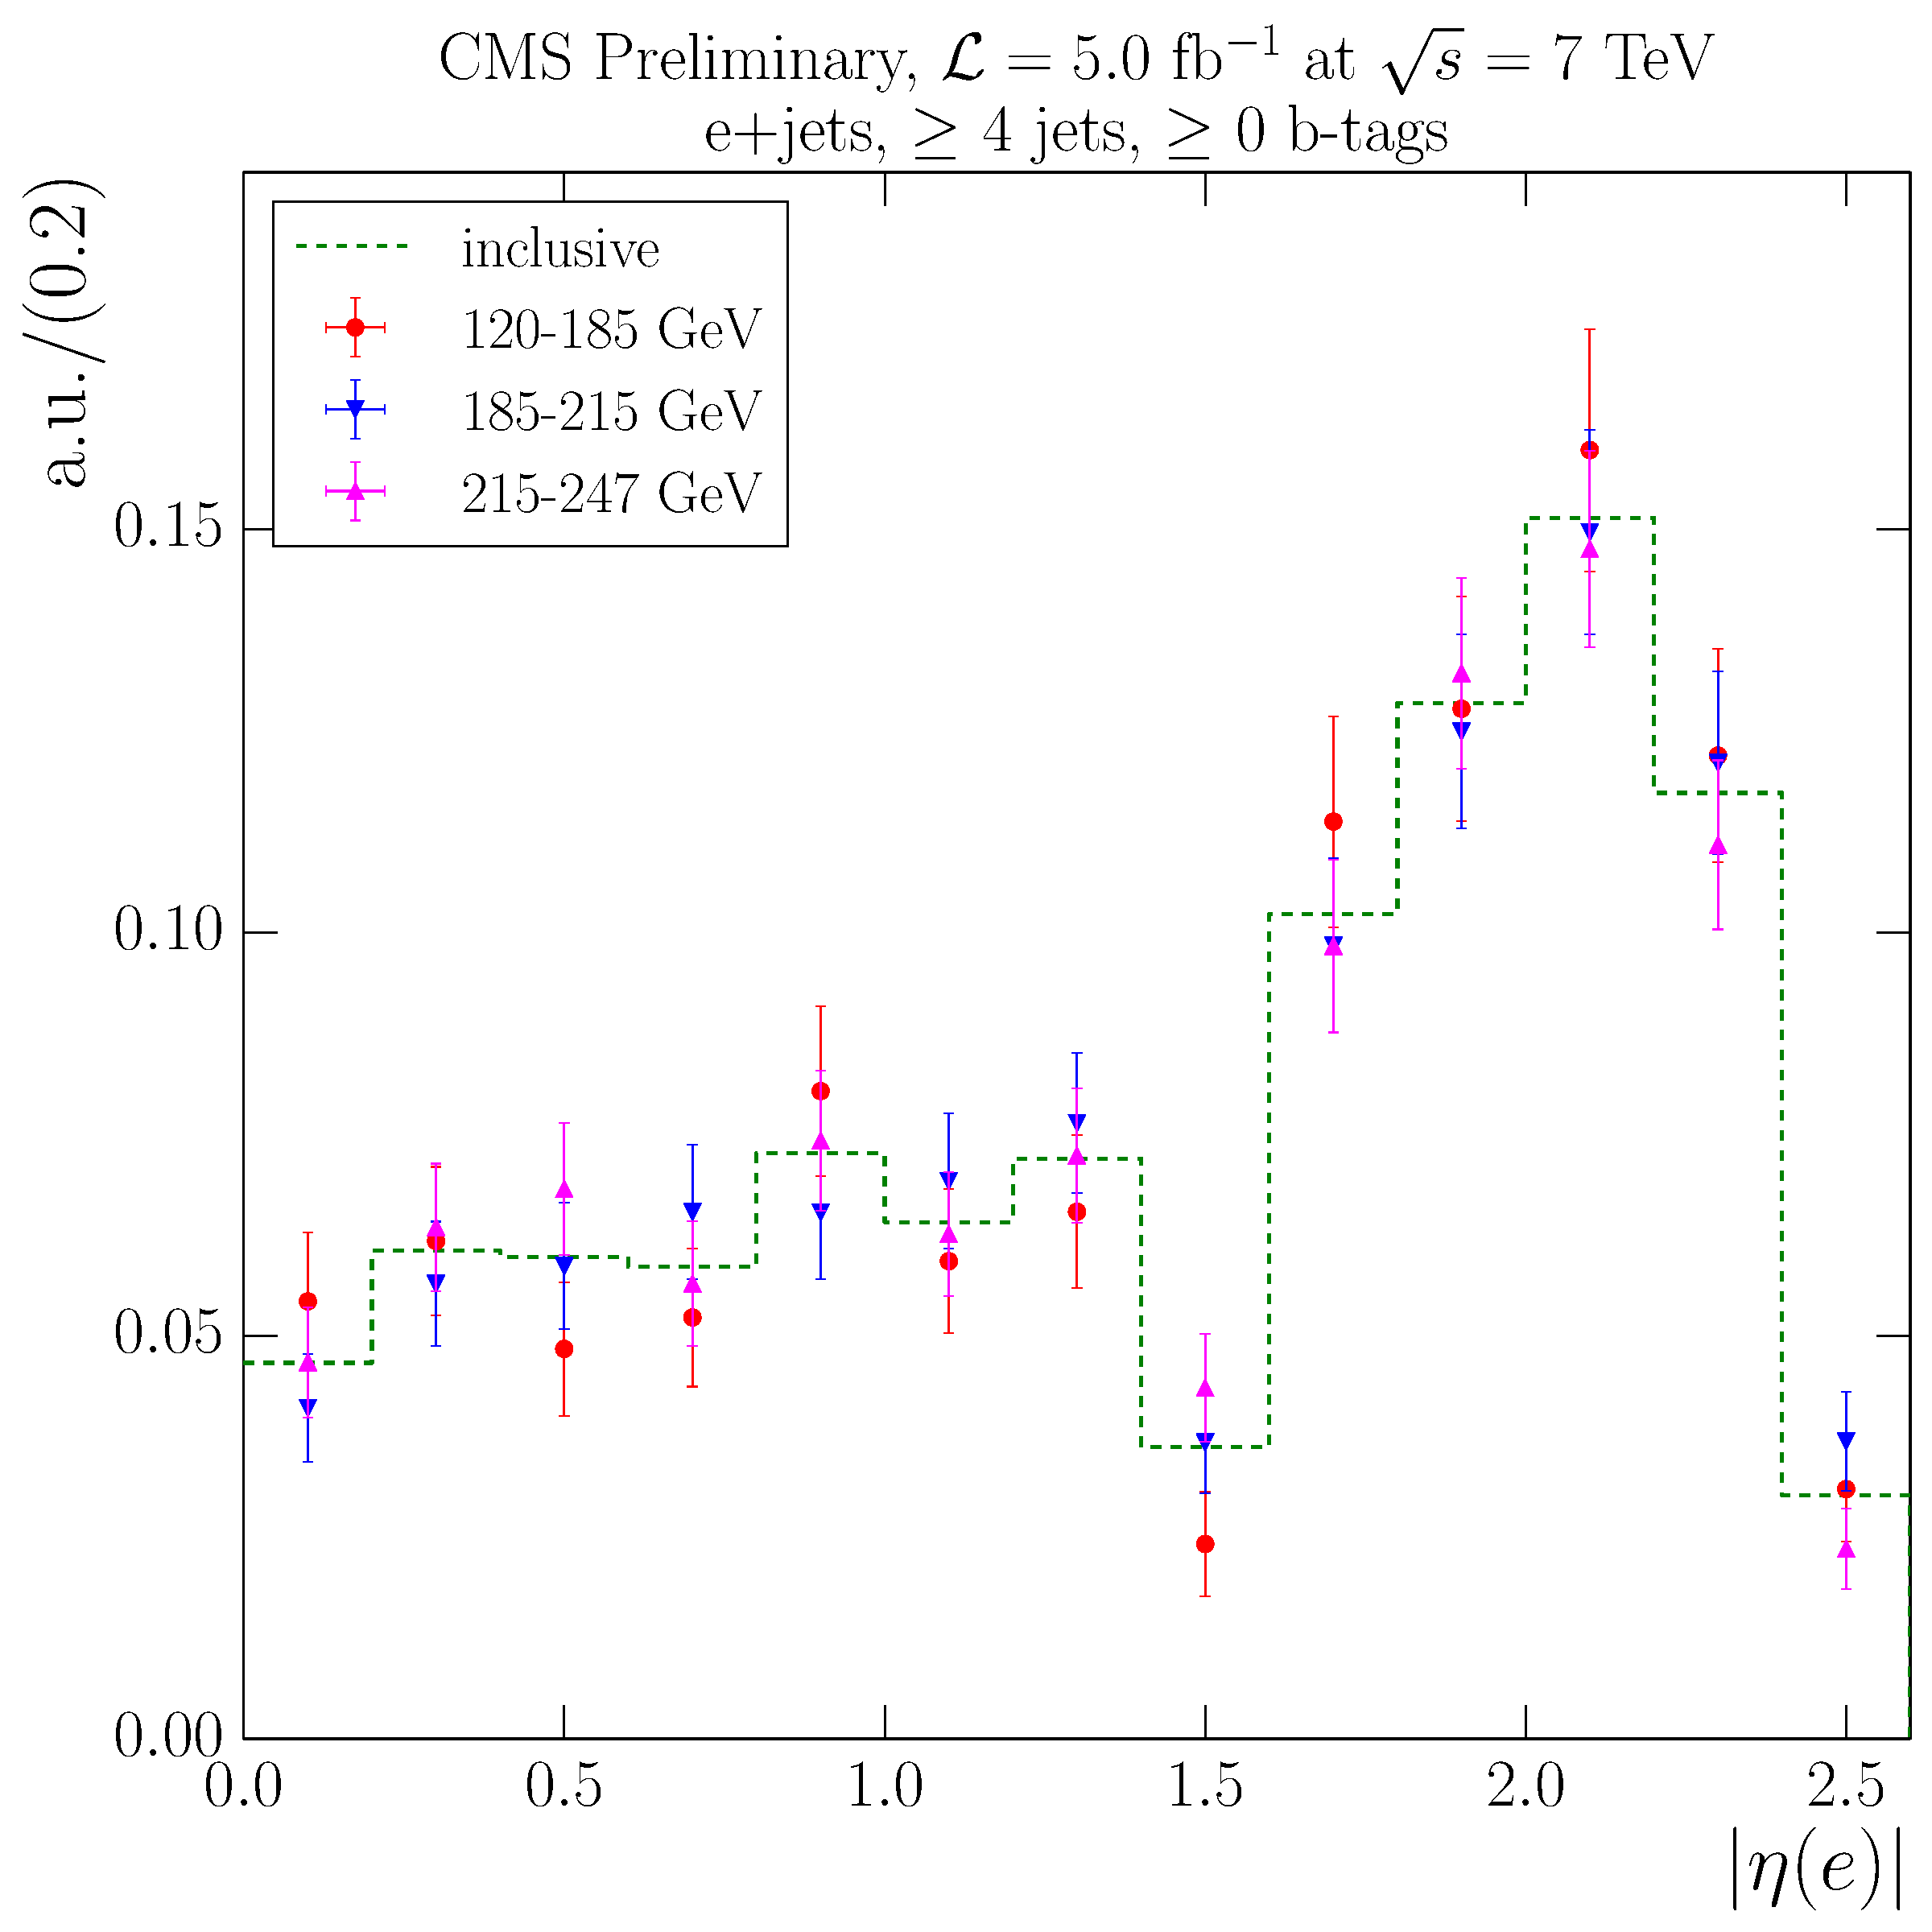
\includegraphics[width=0.48\textwidth]{Chapters/04_Analysis/04b_XSections/images/8TeV/fit_variables/HT/electron_absolute_eta/qcd/HT_electron_absolute_eta_0orMoreBtag_QCD_template_comparison.pdf}\hfill
     
\includegraphics[width=0.48\textwidth]{Chapters/04_Analysis/04b_XSections/images/placeholder.png}\hfill
     %\includegraphics[width=0.48\textwidth]{Chapters/04_Analysis/04b_XSections/images/7TeV/fit_variables/HT/muon_absolute_eta/qcd/HT_inclusive_muon_absolute_eta_2orMoreBtags_templates.pdf}\\    
     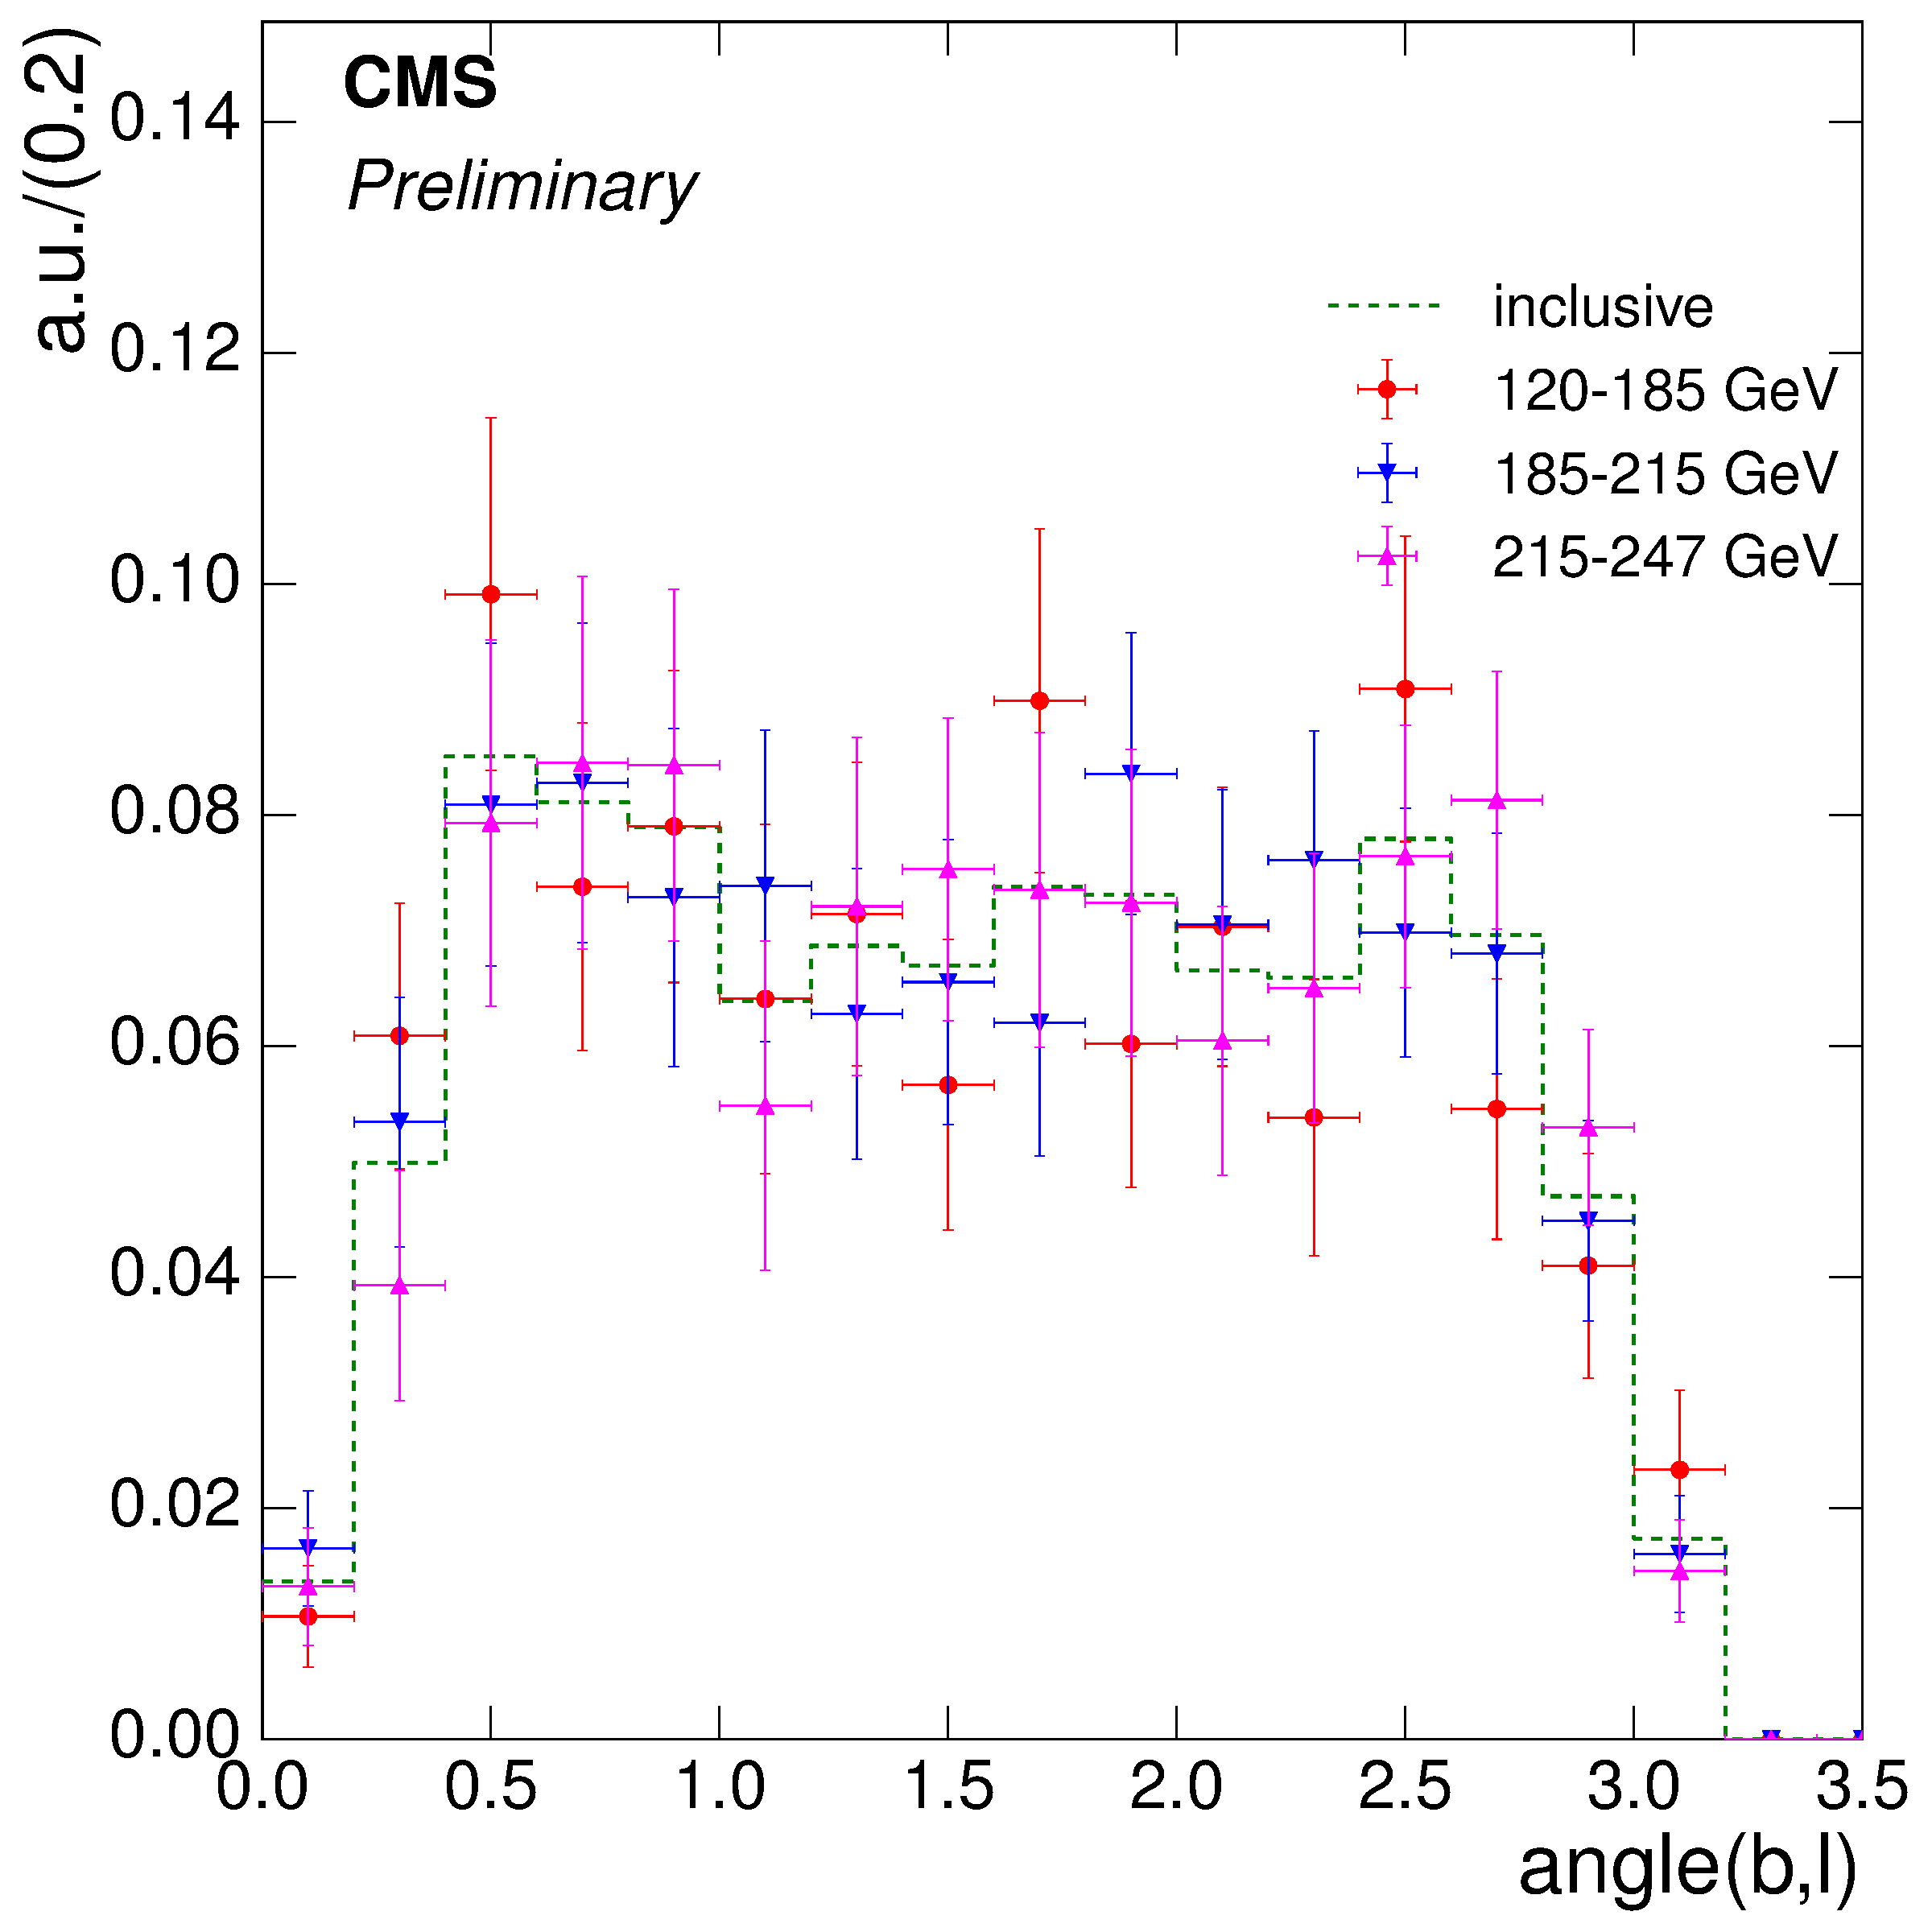
\includegraphics[width=0.48\textwidth]{Chapters/04_Analysis/04b_XSections/images/8TeV/fit_variables/HT/angle_bl/qcd/HT_angle_bl_1orMoreBtag_QCD_template_comparison.pdf}\hfill
     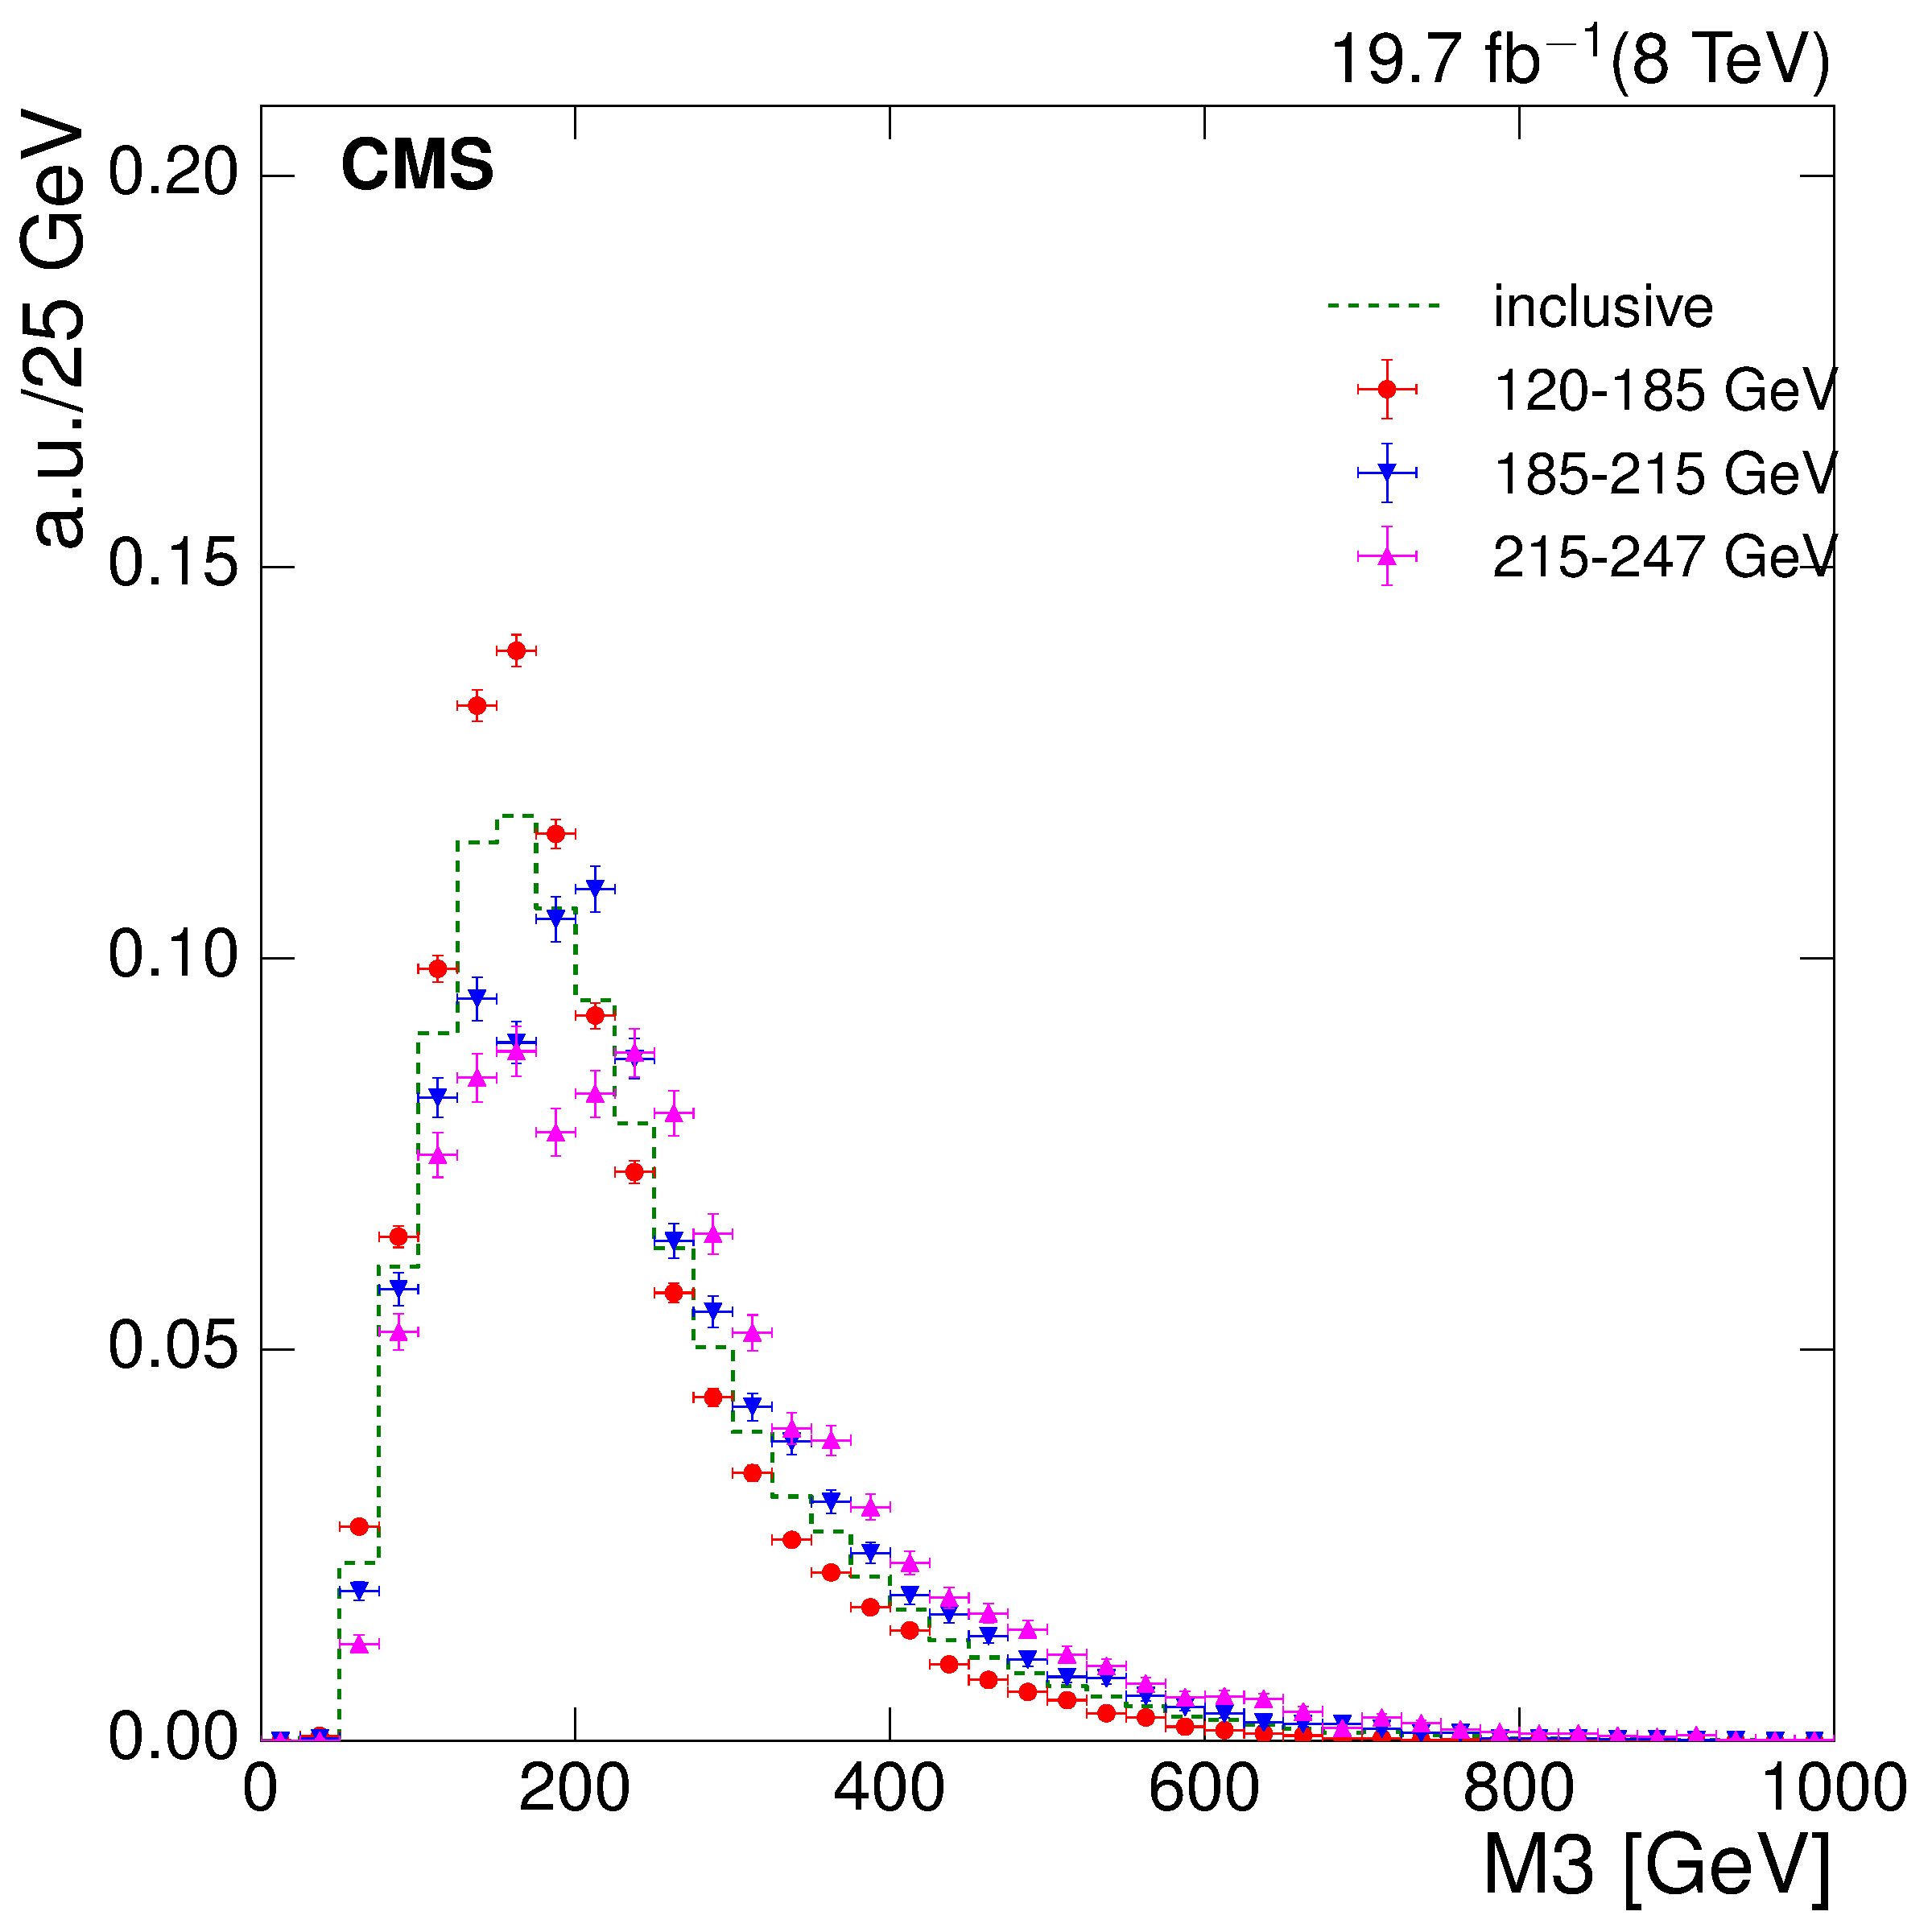
\includegraphics[width=0.48\textwidth]{Chapters/04_Analysis/04b_XSections/images/8TeV/fit_variables/HT/M3/qcd/HT_M3_0orMoreBtag_QCD_template_comparison.pdf}\\
	 \caption{Normalised distributions of the QCD templates for the three fit variables at $\sqrt{s}=8\TeV$
	 inclusive across all \HT bins and for the lowest three \met bins: electron \abseta (upper
	 left), muon \abseta (upper right), $\alpha$ (lower left) and M3 (lower right).}
     \label{fig:HT_fit_variable_qcd_comparisons_8TeV}
\end{figure}

\begin{figure}[hbtp]
    \centering
     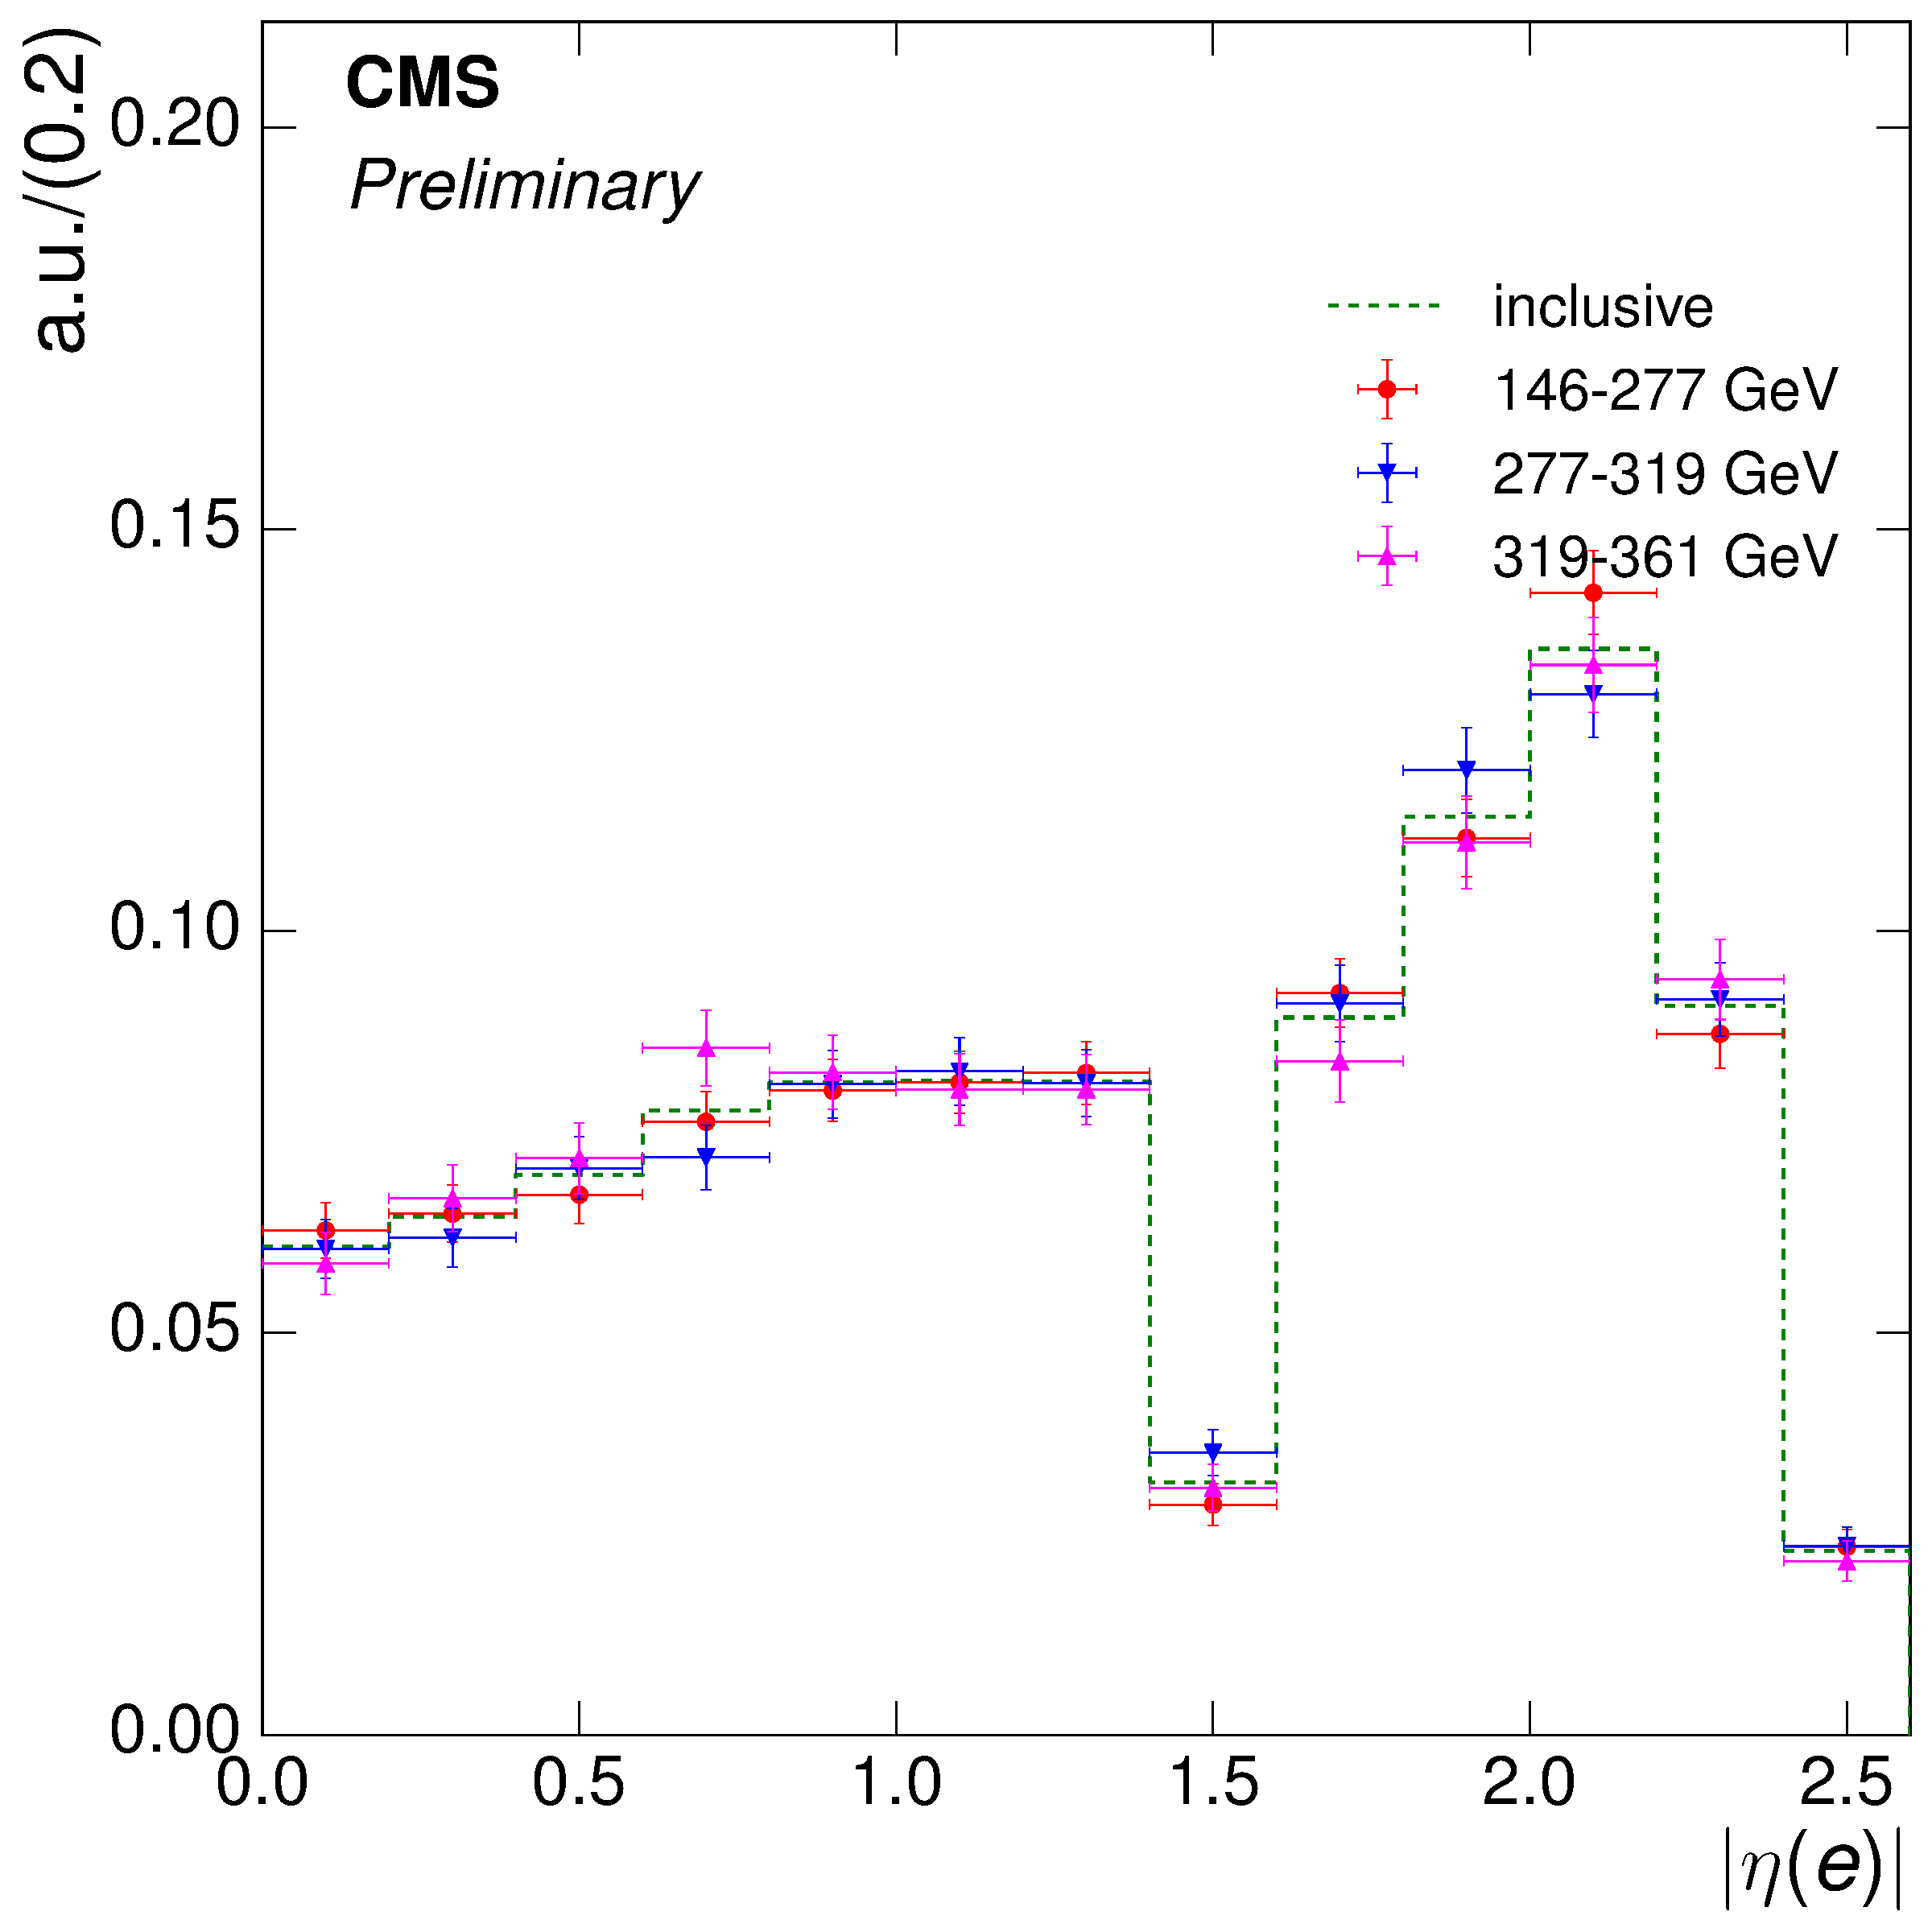
\includegraphics[width=0.48\textwidth]{Chapters/04_Analysis/04b_XSections/images/8TeV/fit_variables/ST/electron_absolute_eta/qcd/ST_electron_absolute_eta_0orMoreBtag_QCD_template_comparison.pdf}\hfill
     
\includegraphics[width=0.48\textwidth]{Chapters/04_Analysis/04b_XSections/images/placeholder.png}\hfill
     %\includegraphics[width=0.48\textwidth]{Chapters/04_Analysis/04b_XSections/images/7TeV/fit_variables/ST/muon_absolute_eta/qcd/ST_inclusive_muon_absolute_eta_2orMoreBtags_templates.pdf}\\    
     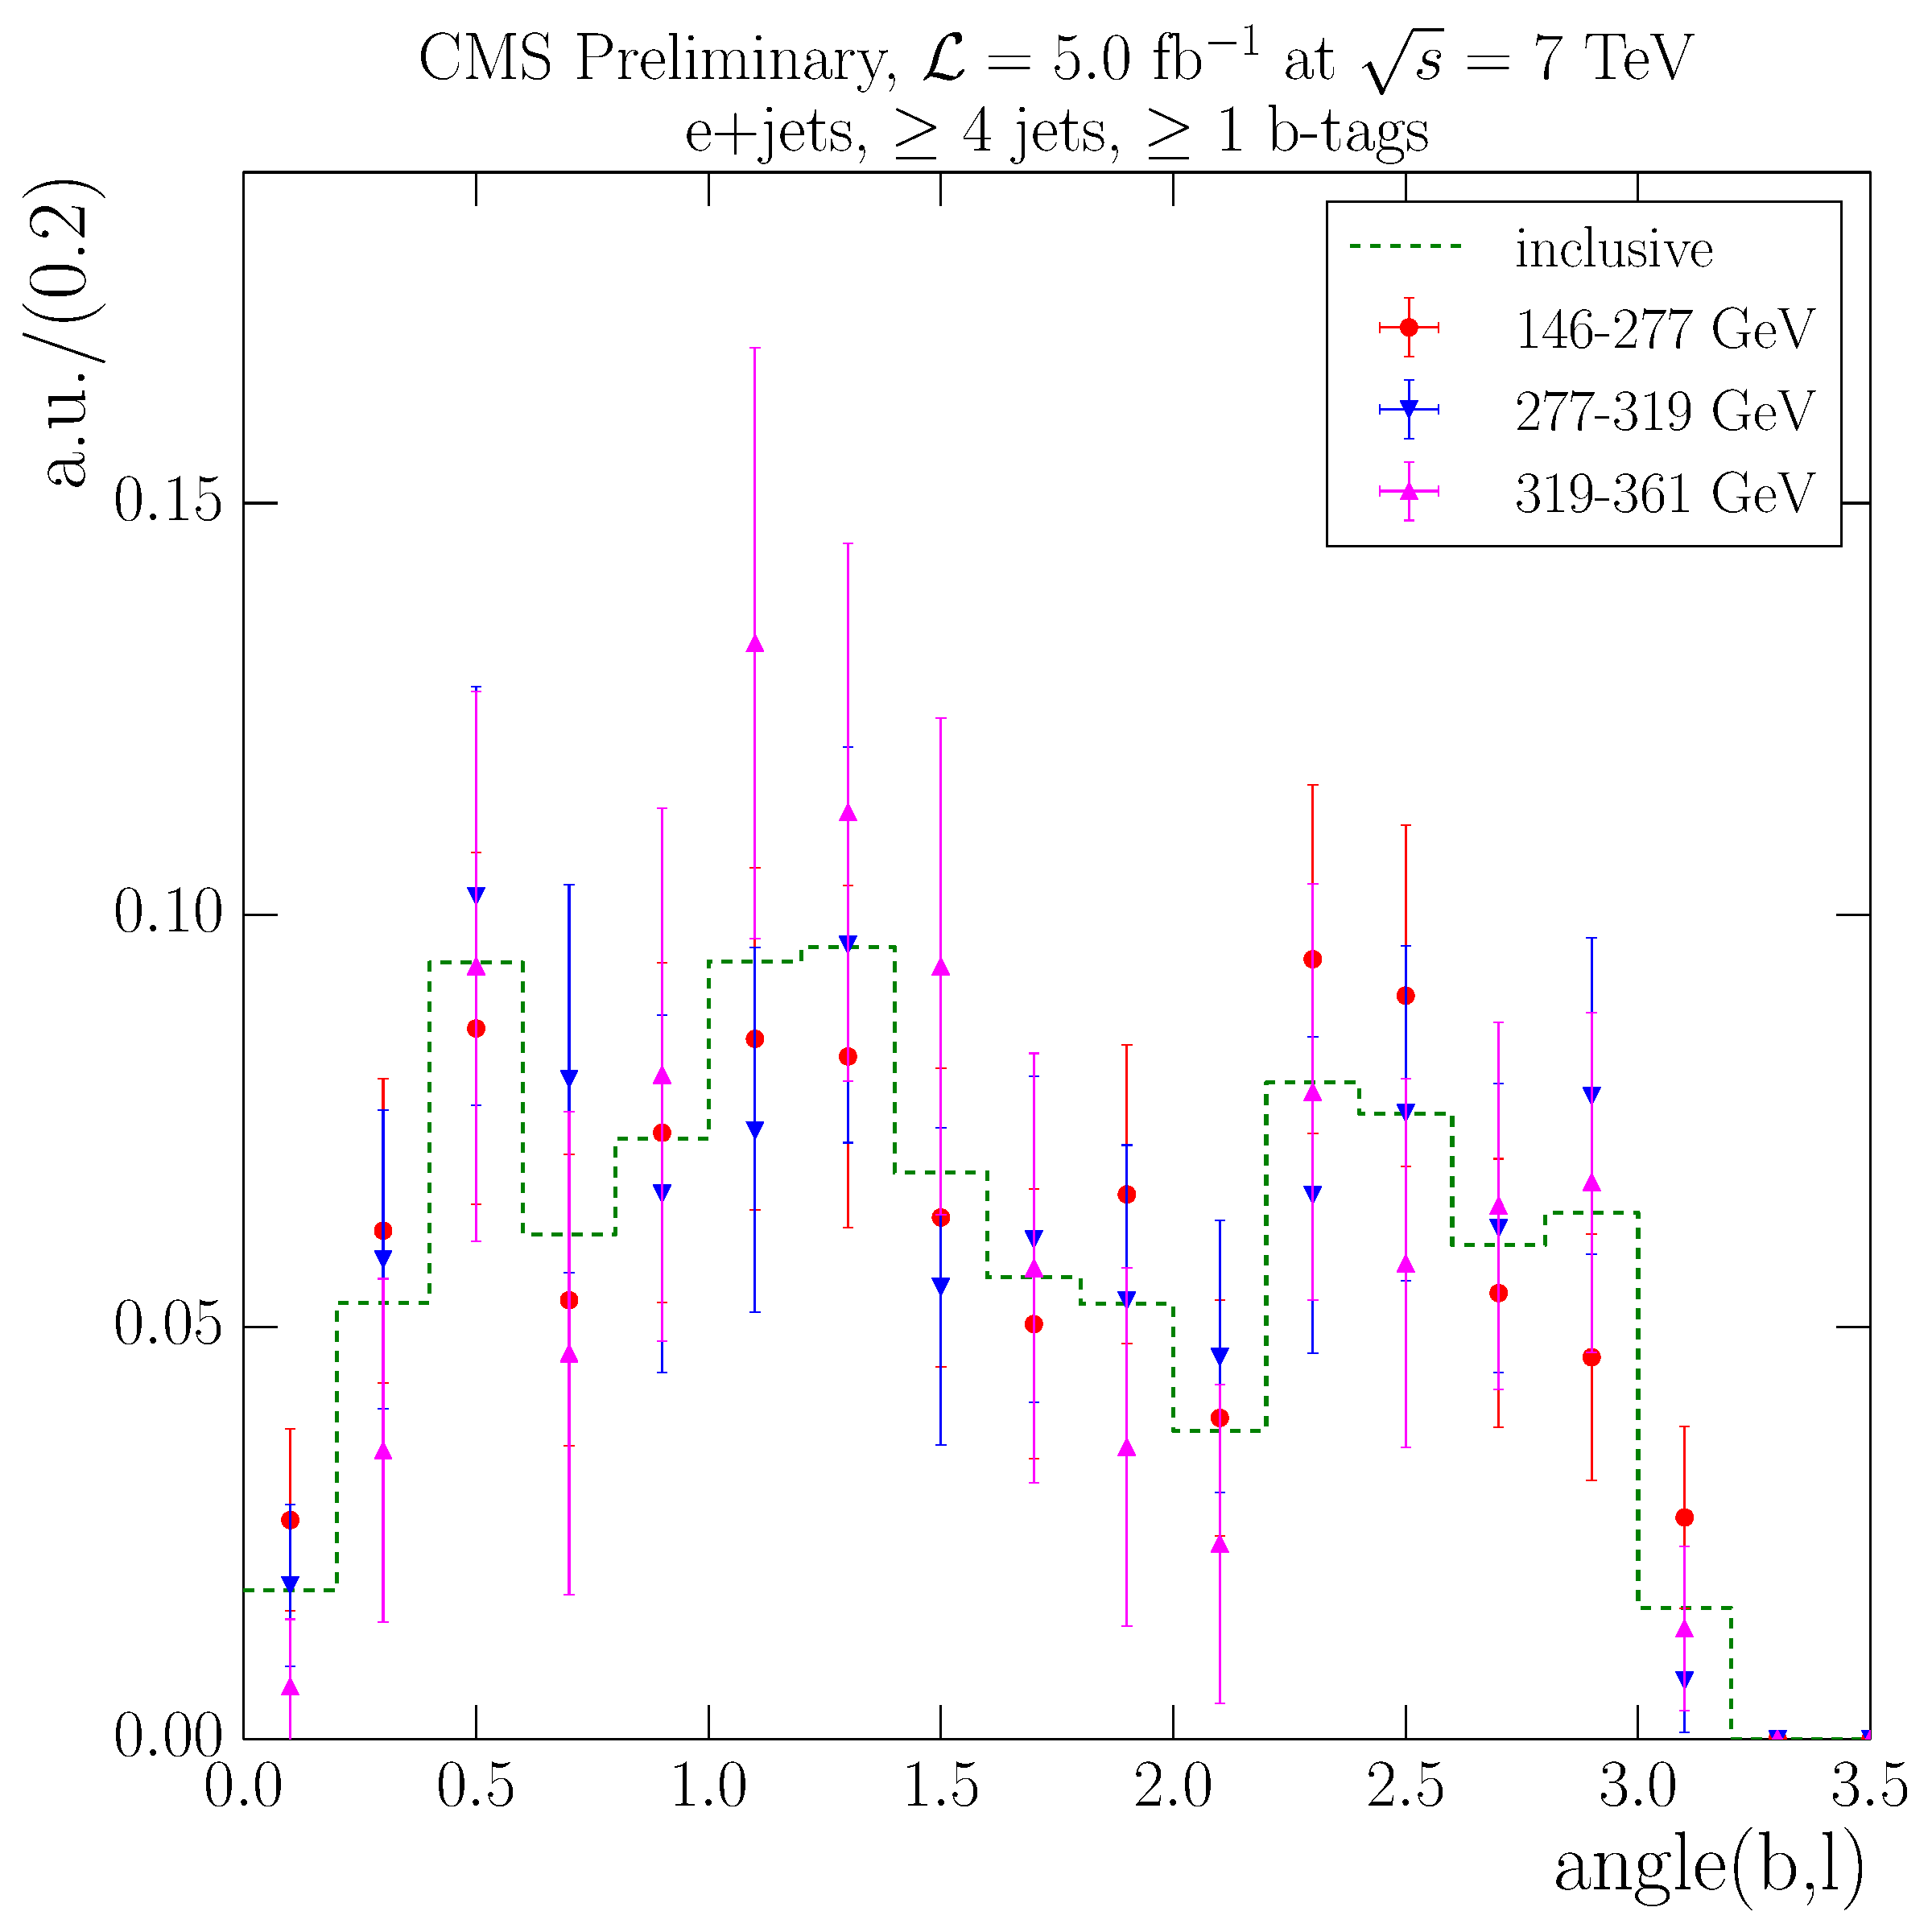
\includegraphics[width=0.48\textwidth]{Chapters/04_Analysis/04b_XSections/images/8TeV/fit_variables/ST/angle_bl/qcd/ST_angle_bl_1orMoreBtag_QCD_template_comparison.pdf}\hfill
     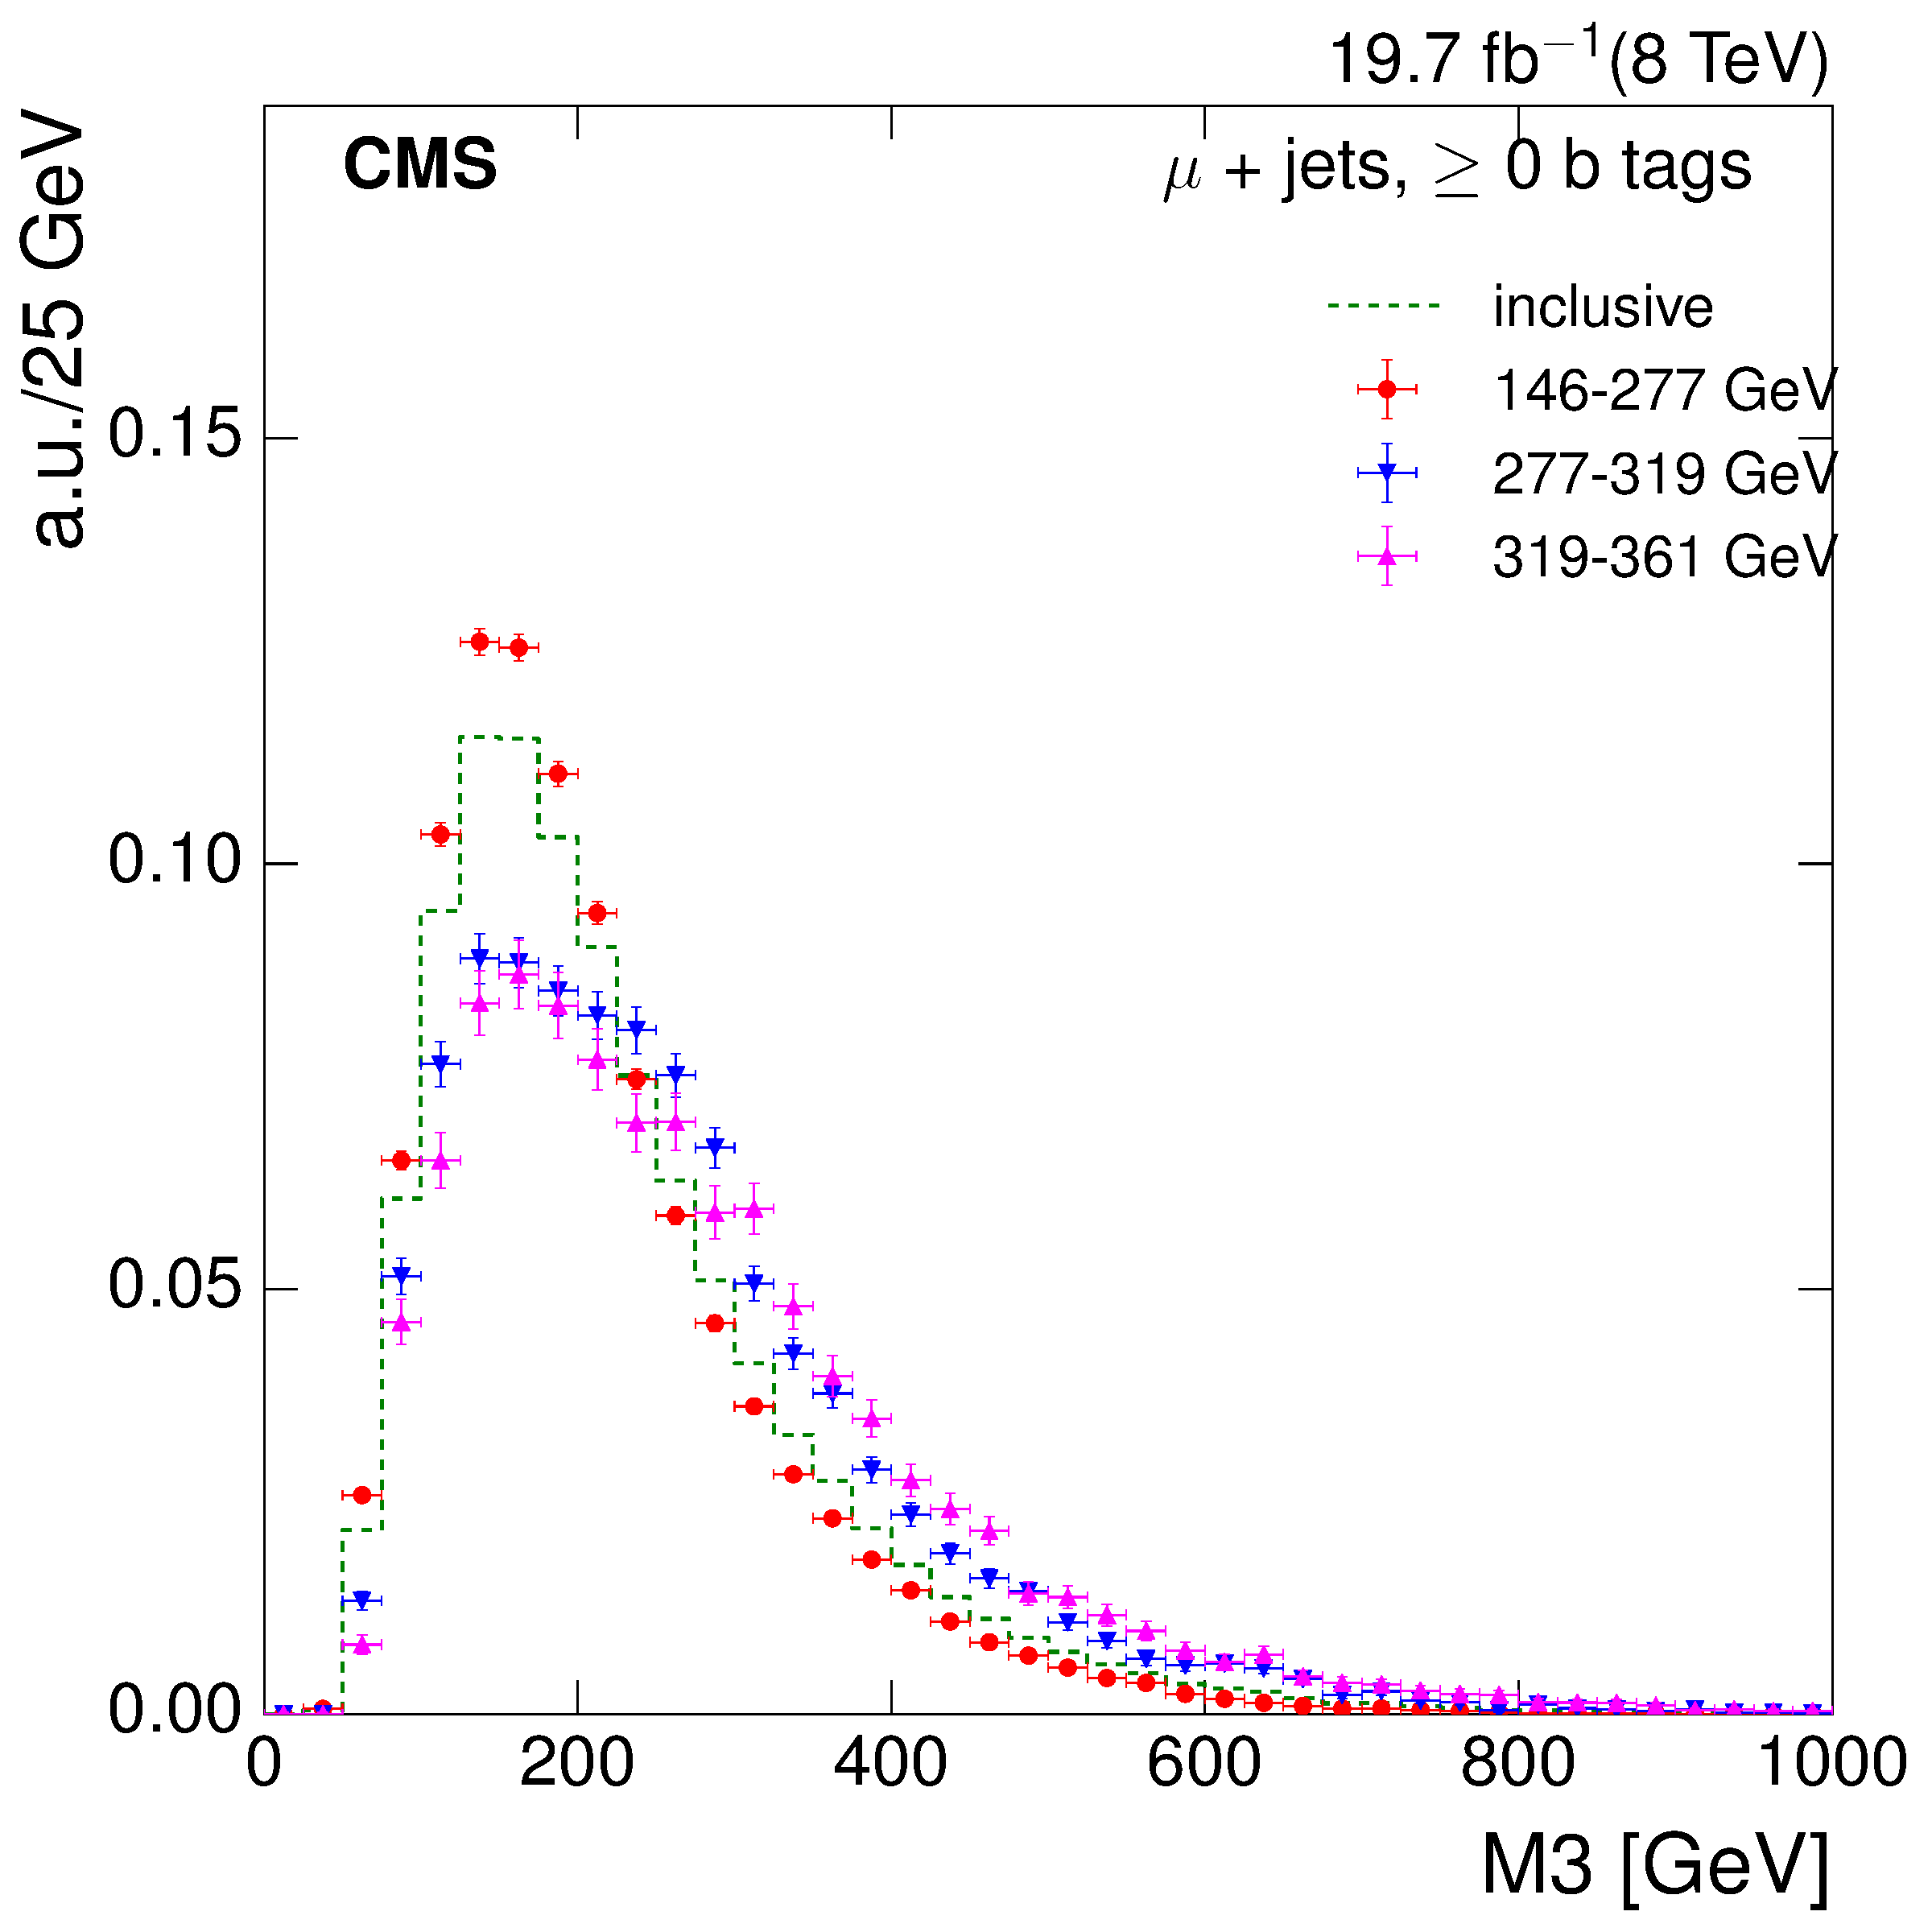
\includegraphics[width=0.48\textwidth]{Chapters/04_Analysis/04b_XSections/images/8TeV/fit_variables/ST/M3/qcd/ST_M3_0orMoreBtag_QCD_template_comparison.pdf}\\
	 \caption{Normalised distributions of the QCD templates for the three fit variables at $\sqrt{s}=8\TeV$
	 inclusive across all \st bins and for the lowest three \st bins: electron \abseta (upper
	 left), muon \abseta (upper right), $\alpha$ (lower left) and M3 (lower right).}
     \label{fig:ST_fit_variable_qcd_comparisons_8TeV}
\end{figure}

\begin{figure}[hbtp]
    \centering
     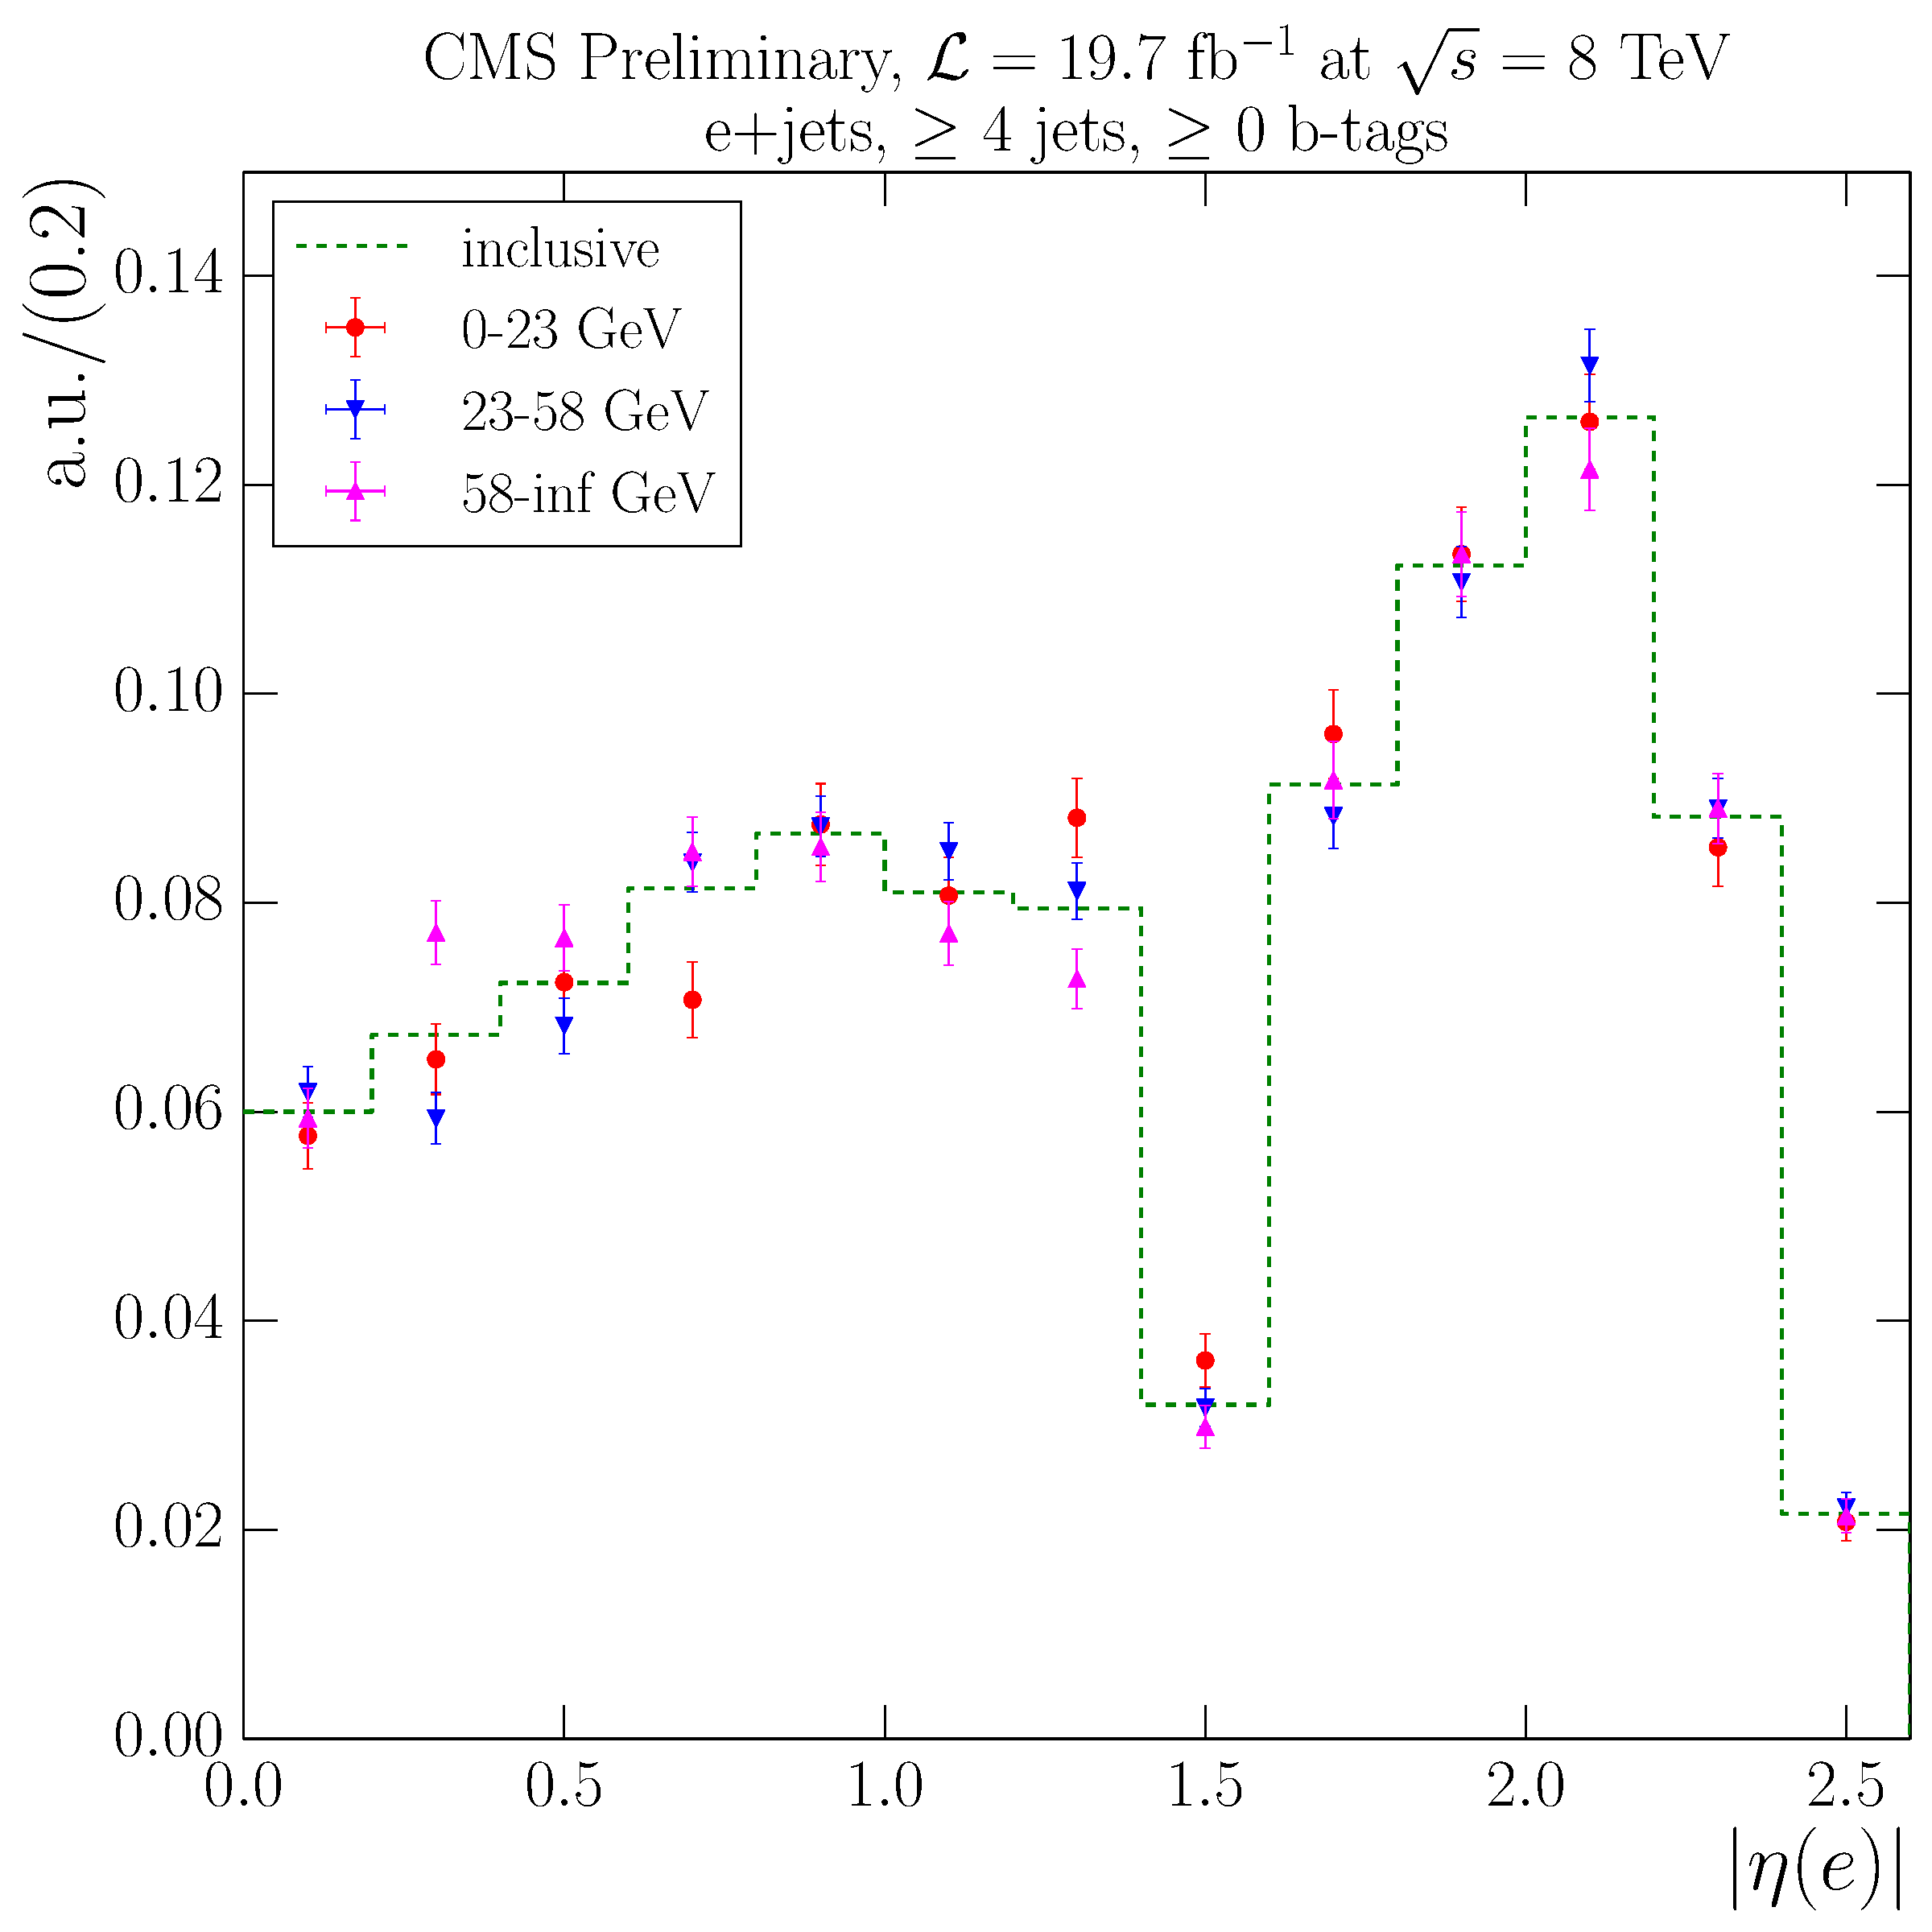
\includegraphics[width=0.48\textwidth]{Chapters/04_Analysis/04b_XSections/images/8TeV/fit_variables/MT/electron_absolute_eta/qcd/MT_electron_absolute_eta_0orMoreBtag_QCD_template_comparison.pdf}\hfill
     
\includegraphics[width=0.48\textwidth]{Chapters/04_Analysis/04b_XSections/images/placeholder.png}\hfill
     %\includegraphics[width=0.48\textwidth]{Chapters/04_Analysis/04b_XSections/images/7TeV/fit_variables/MT/muon_absolute_eta/qcd/MT_inclusive_muon_absolute_eta_2orMoreBtags_templates.pdf}\\    
     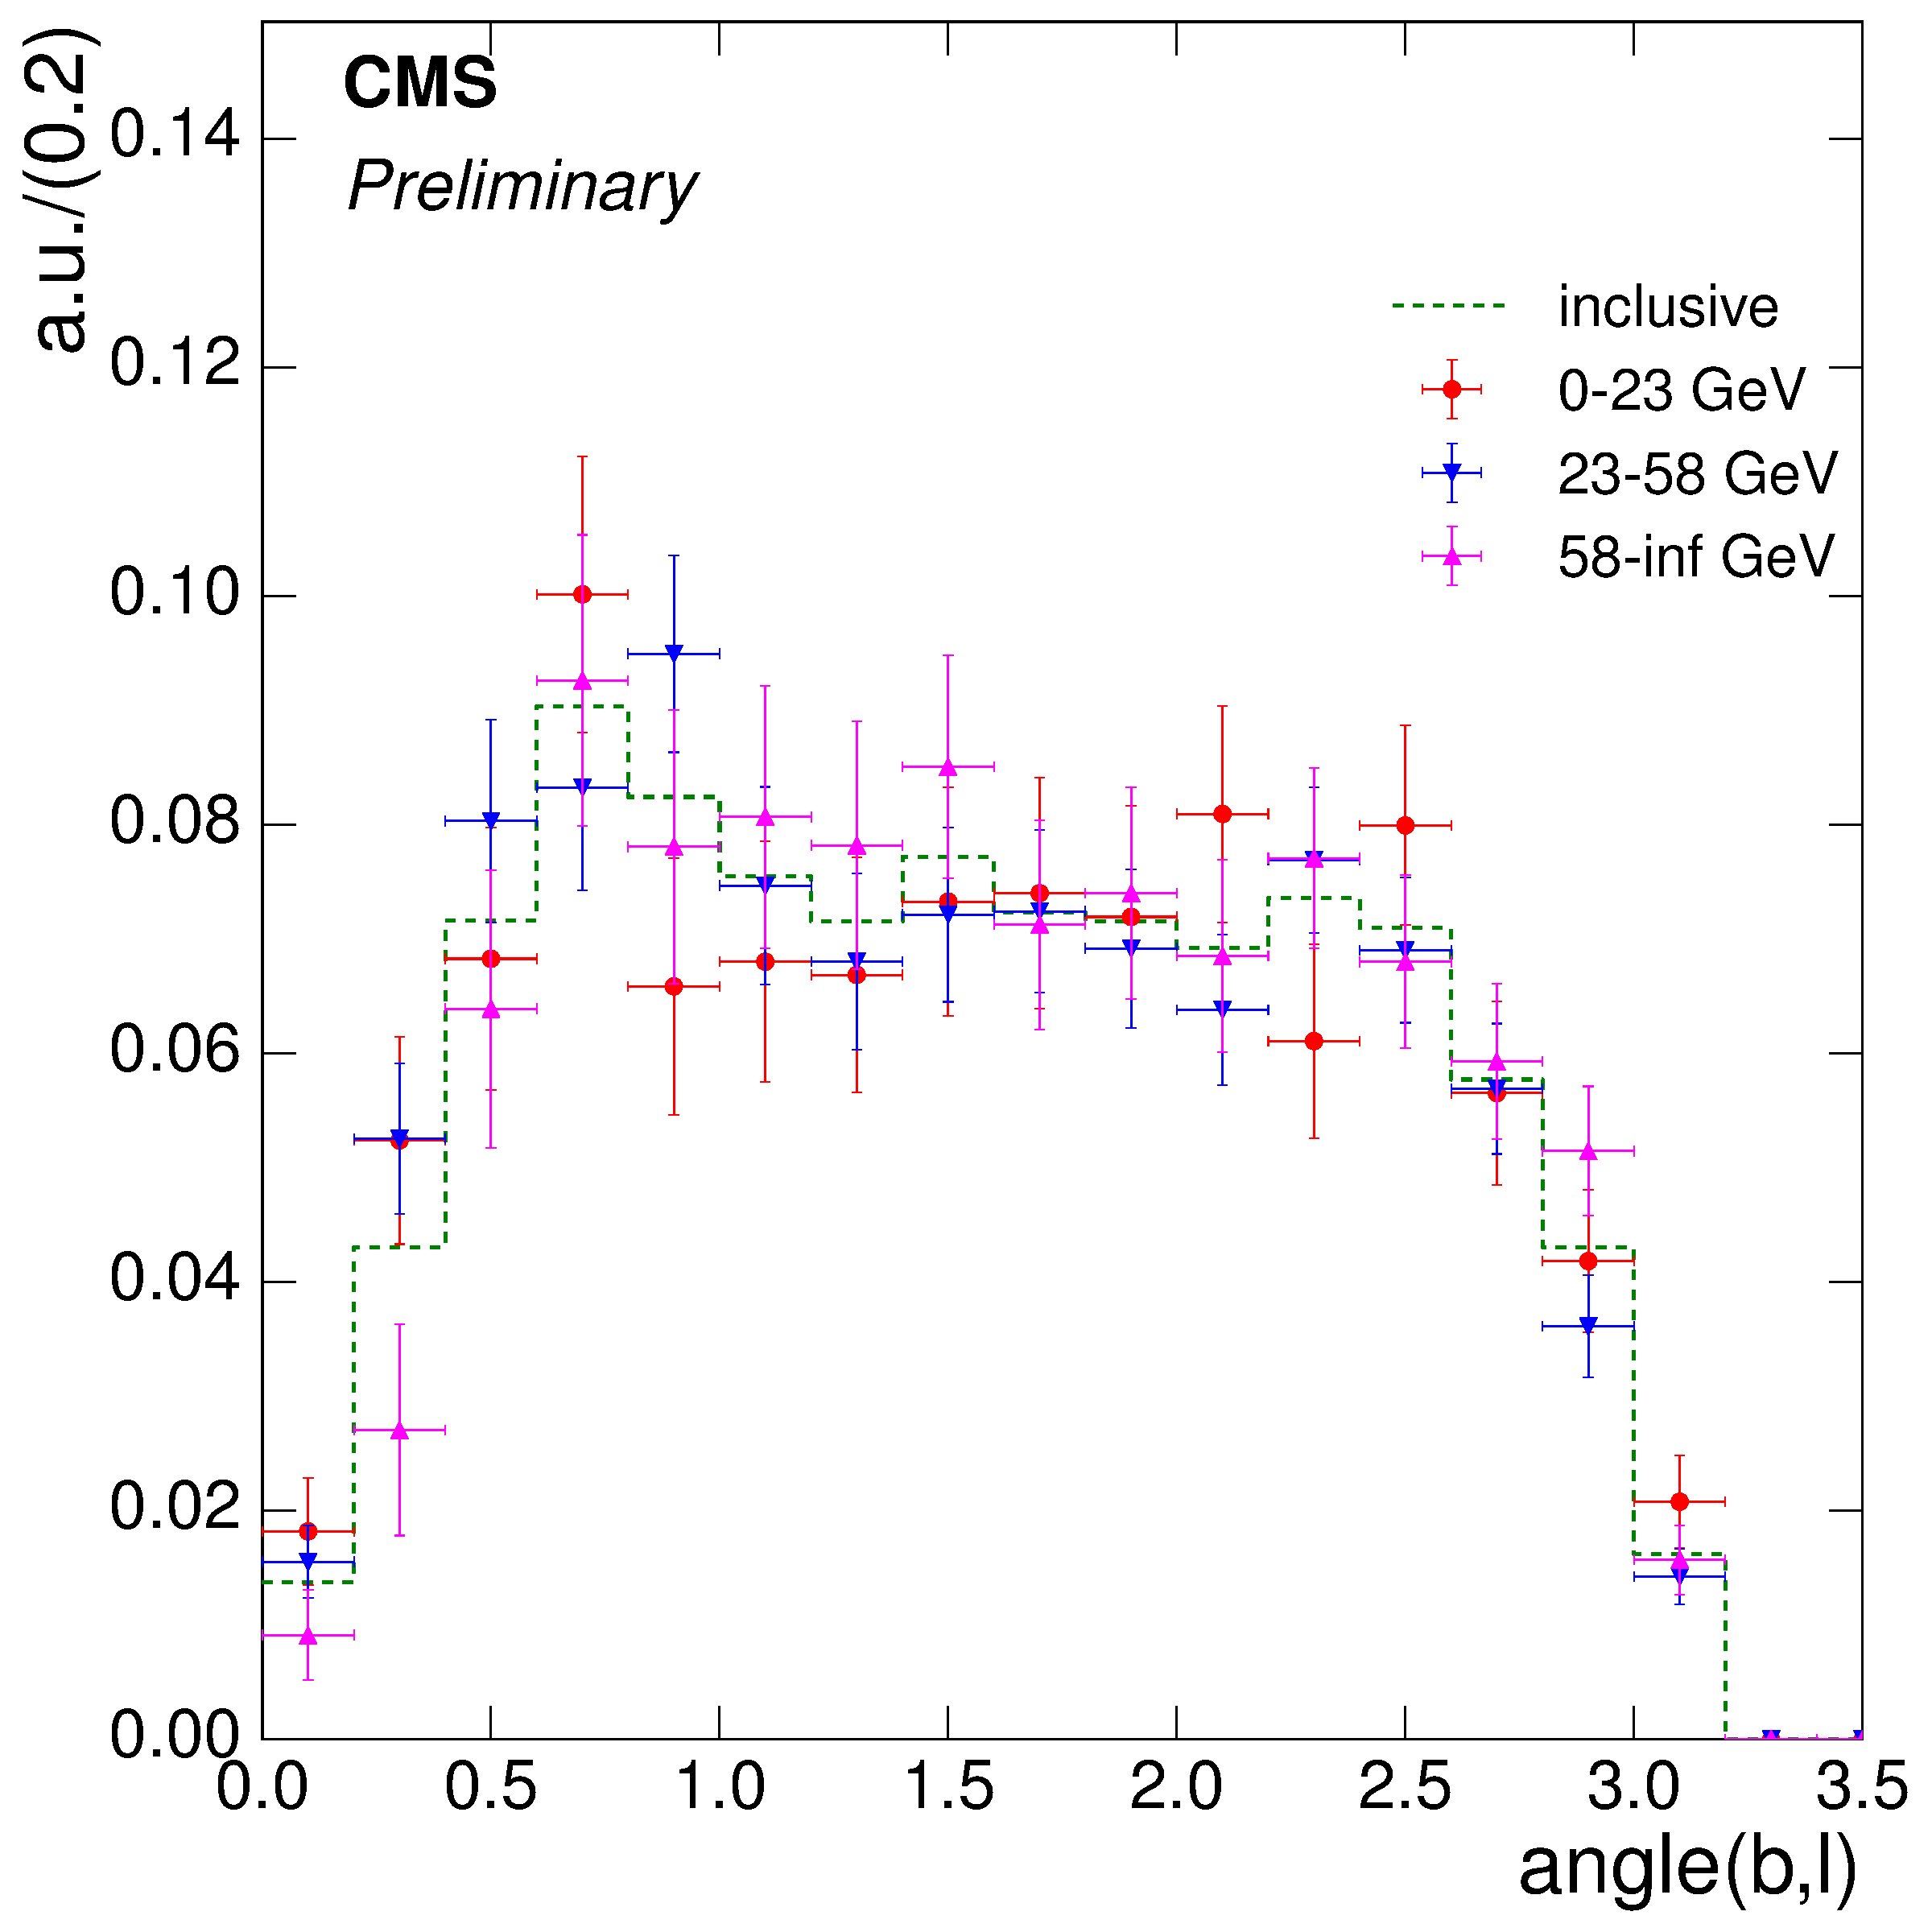
\includegraphics[width=0.48\textwidth]{Chapters/04_Analysis/04b_XSections/images/8TeV/fit_variables/MT/angle_bl/qcd/MT_angle_bl_1orMoreBtag_QCD_template_comparison.pdf}\hfill
     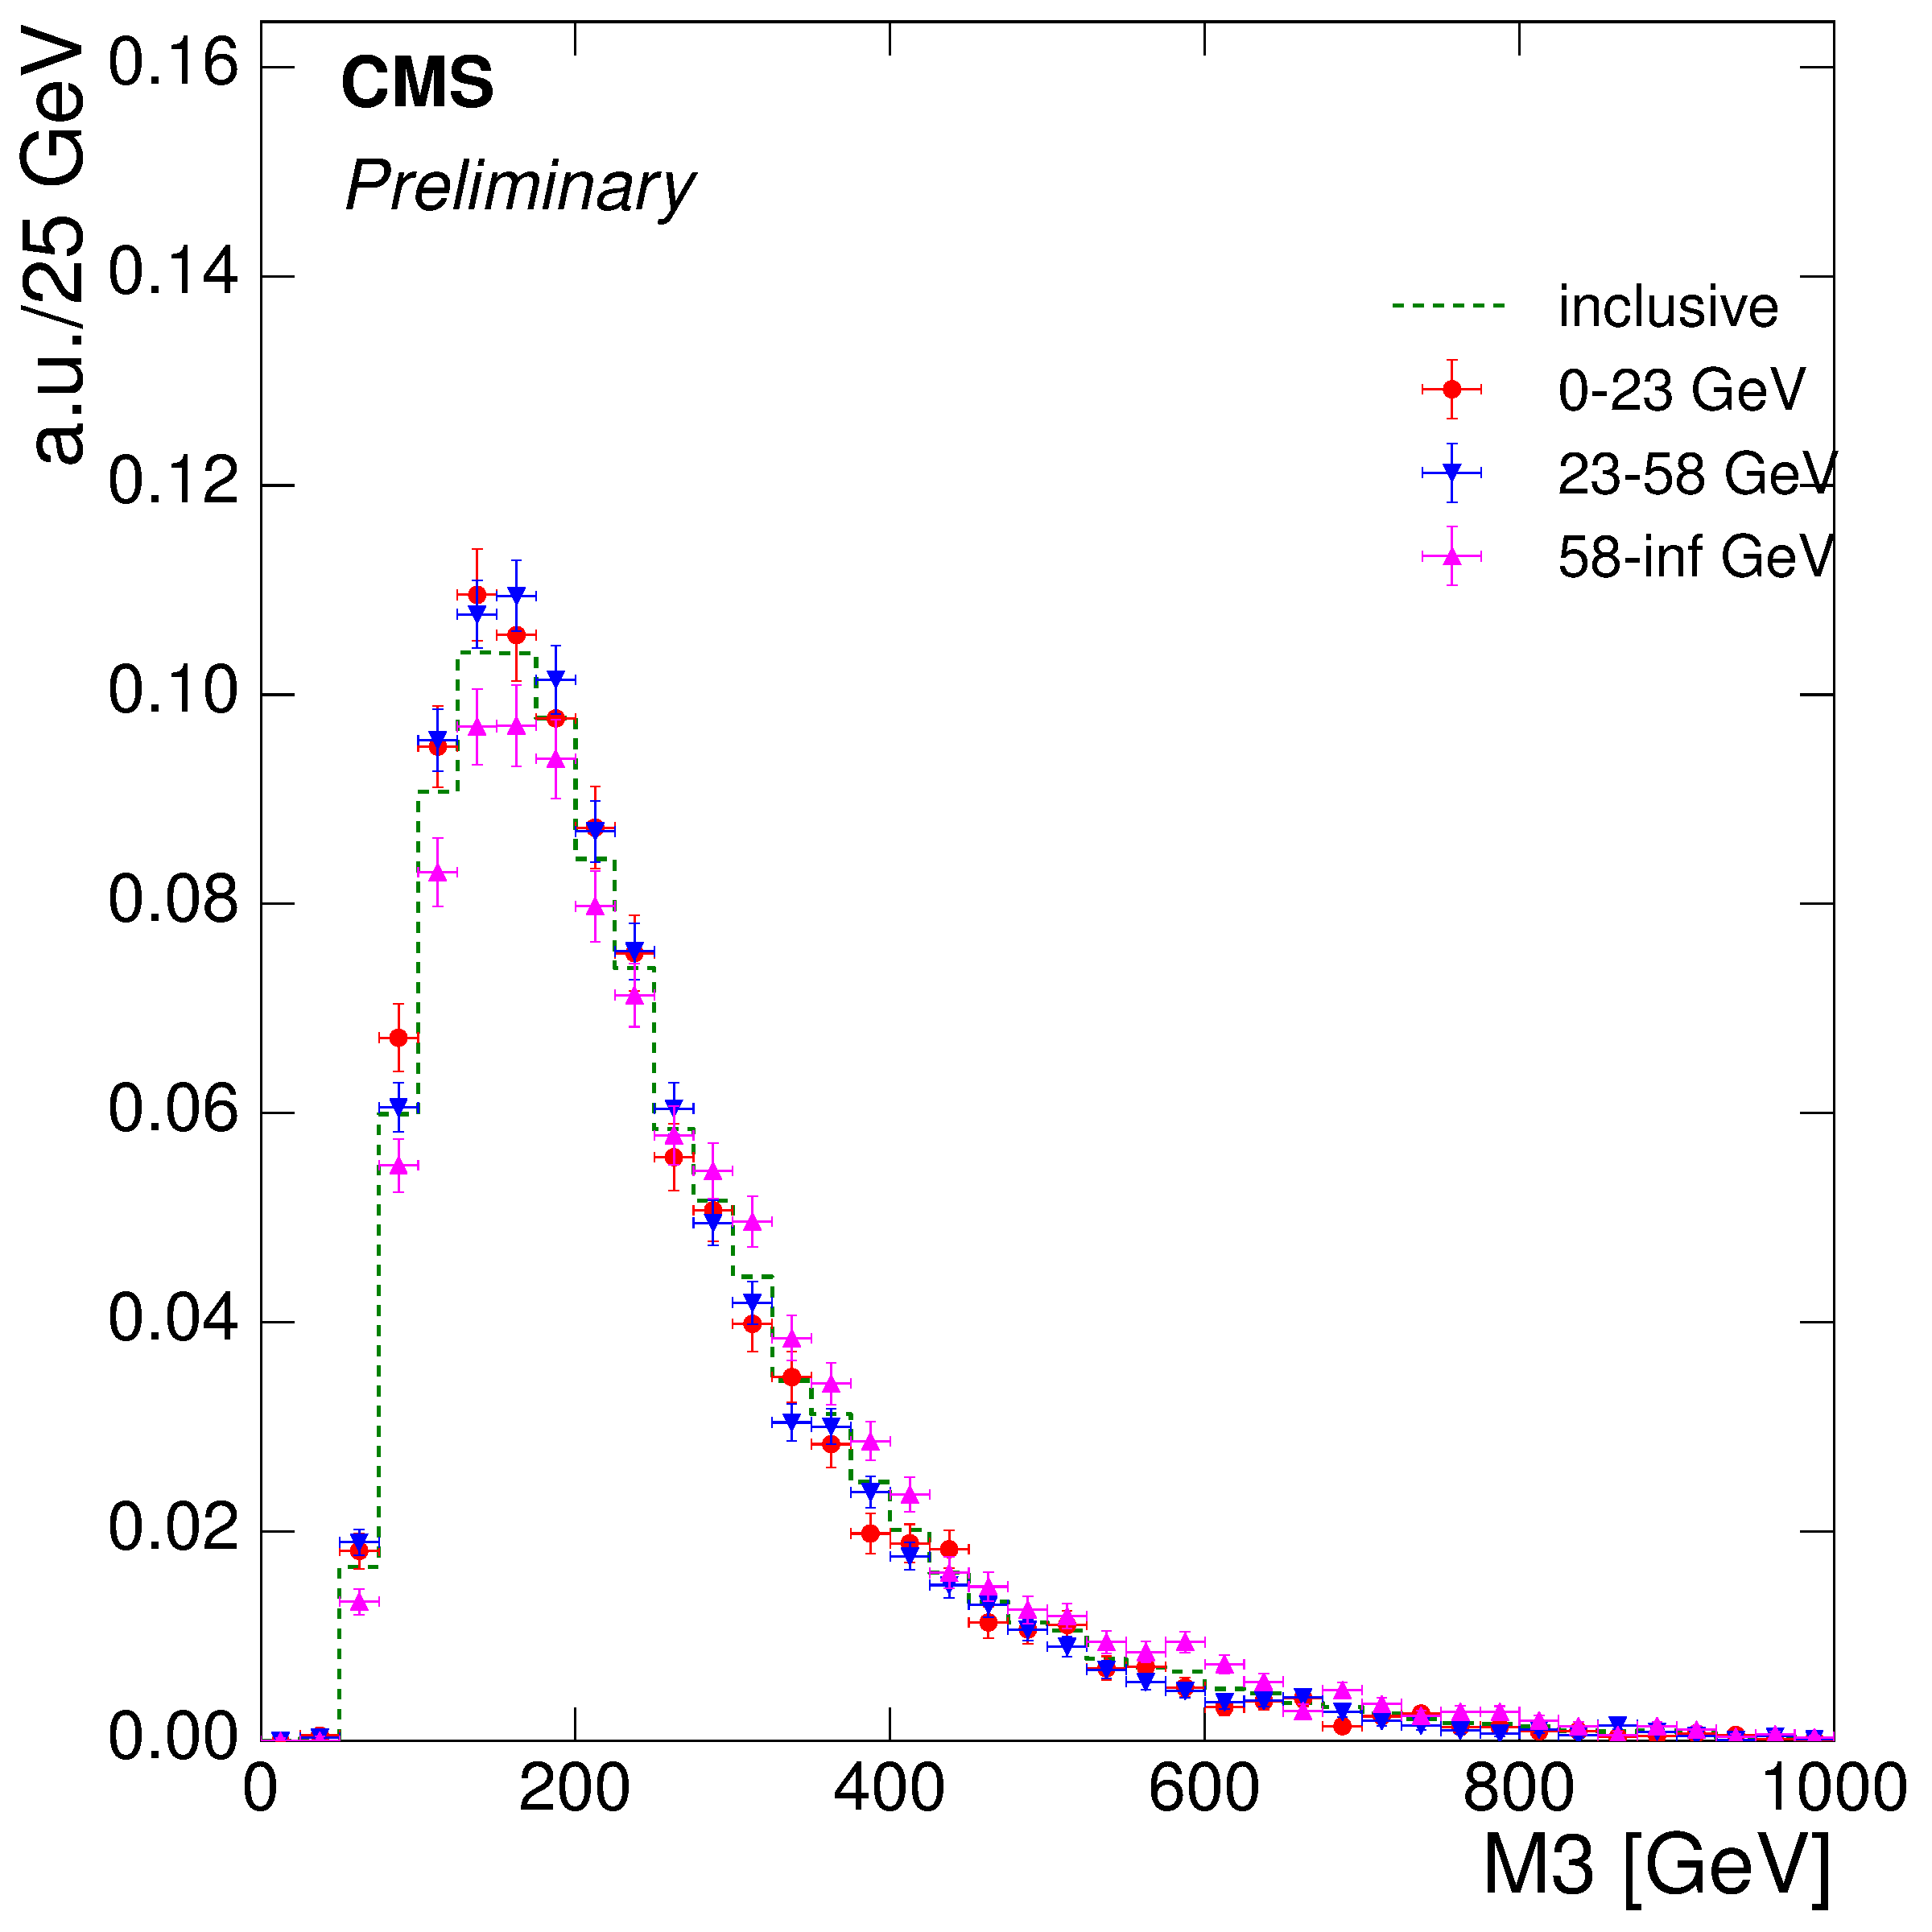
\includegraphics[width=0.48\textwidth]{Chapters/04_Analysis/04b_XSections/images/8TeV/fit_variables/MT/M3/qcd/MT_M3_0orMoreBtag_QCD_template_comparison.pdf}\\
	 \caption{Normalised distributions of the QCD templates for the three fit variables at $\sqrt{s}=8\TeV$
	 inclusive across all \mt bins and for the lowest three \mt bins: electron \abseta (upper
	 left), muon \abseta (upper right), $\alpha$ (lower left) and M3 (lower right).}
     \label{fig:MT_fit_variable_qcd_comparisons_8TeV}
\end{figure}

\begin{figure}[hbtp]
    \centering
     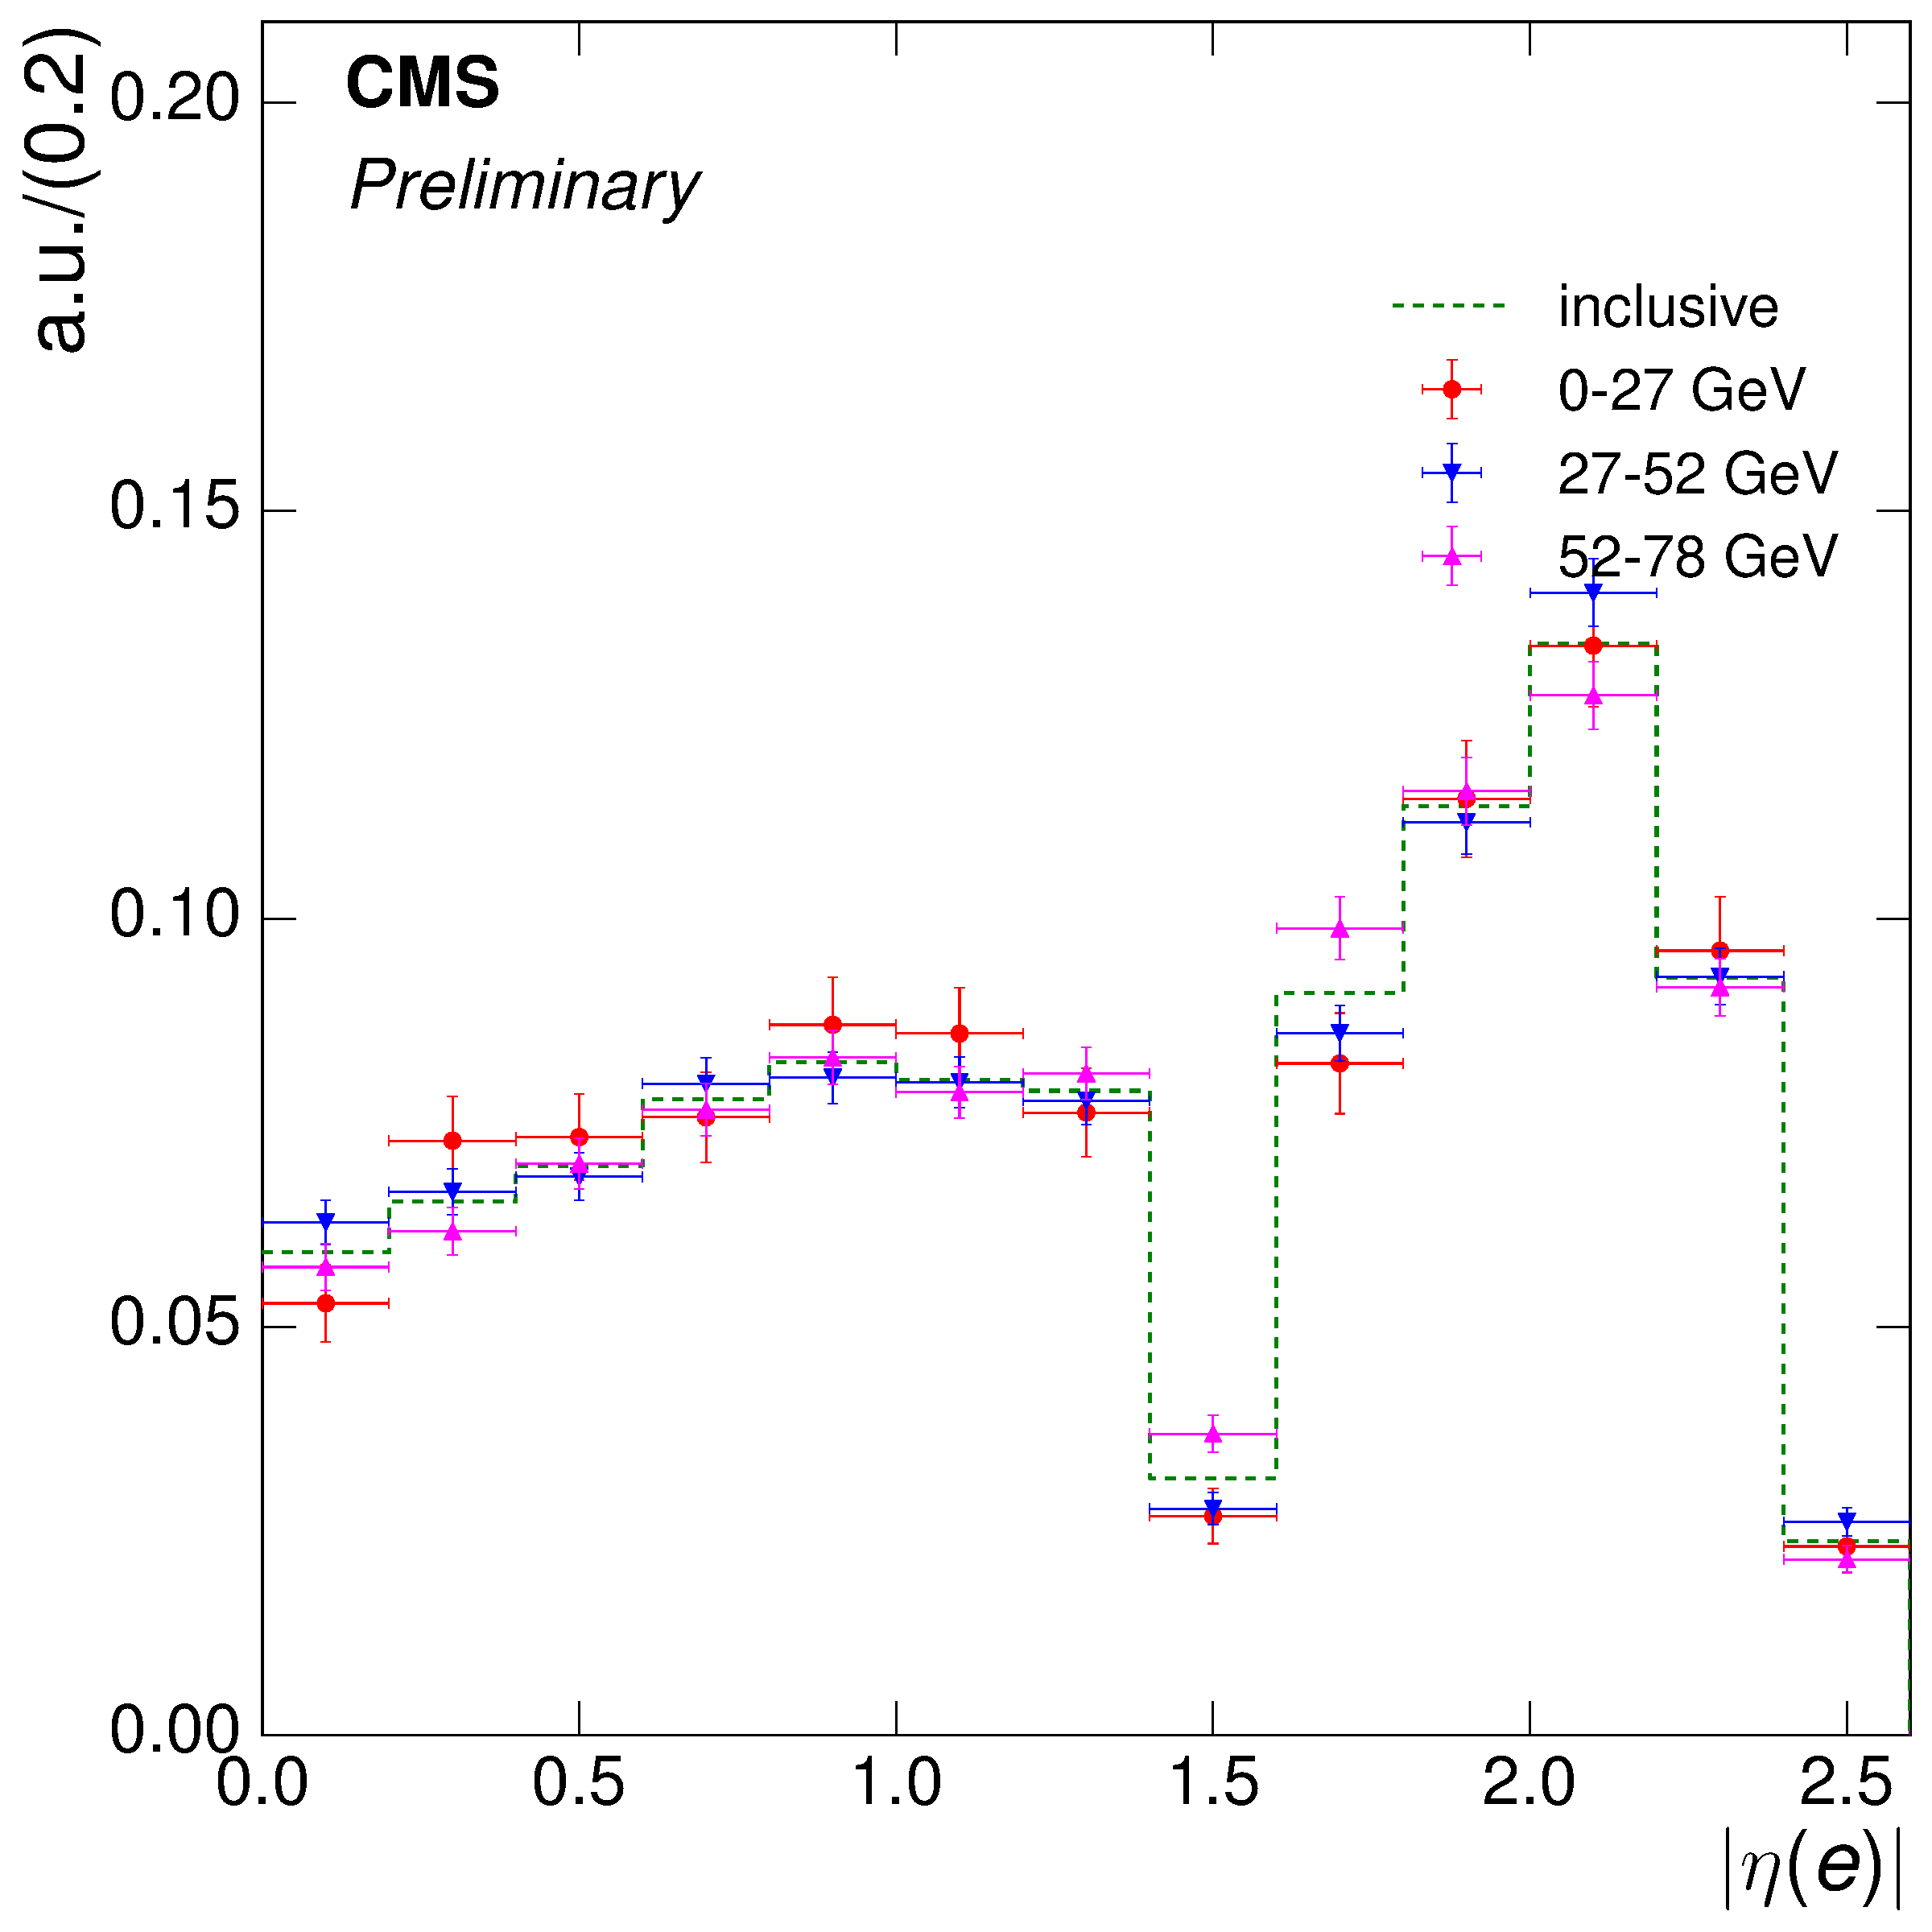
\includegraphics[width=0.48\textwidth]{Chapters/04_Analysis/04b_XSections/images/8TeV/fit_variables/WPT/electron_absolute_eta/qcd/WPT_electron_absolute_eta_0orMoreBtag_QCD_template_comparison.pdf}\hfill
     
\includegraphics[width=0.48\textwidth]{Chapters/04_Analysis/04b_XSections/images/placeholder.png}\hfill
     %\includegraphics[width=0.48\textwidth]{Chapters/04_Analysis/04b_XSections/images/7TeV/fit_variables/WPT/muon_absolute_eta/qcd/WPT_inclusive_muon_absolute_eta_2orMoreBtags_templates.pdf}\\
     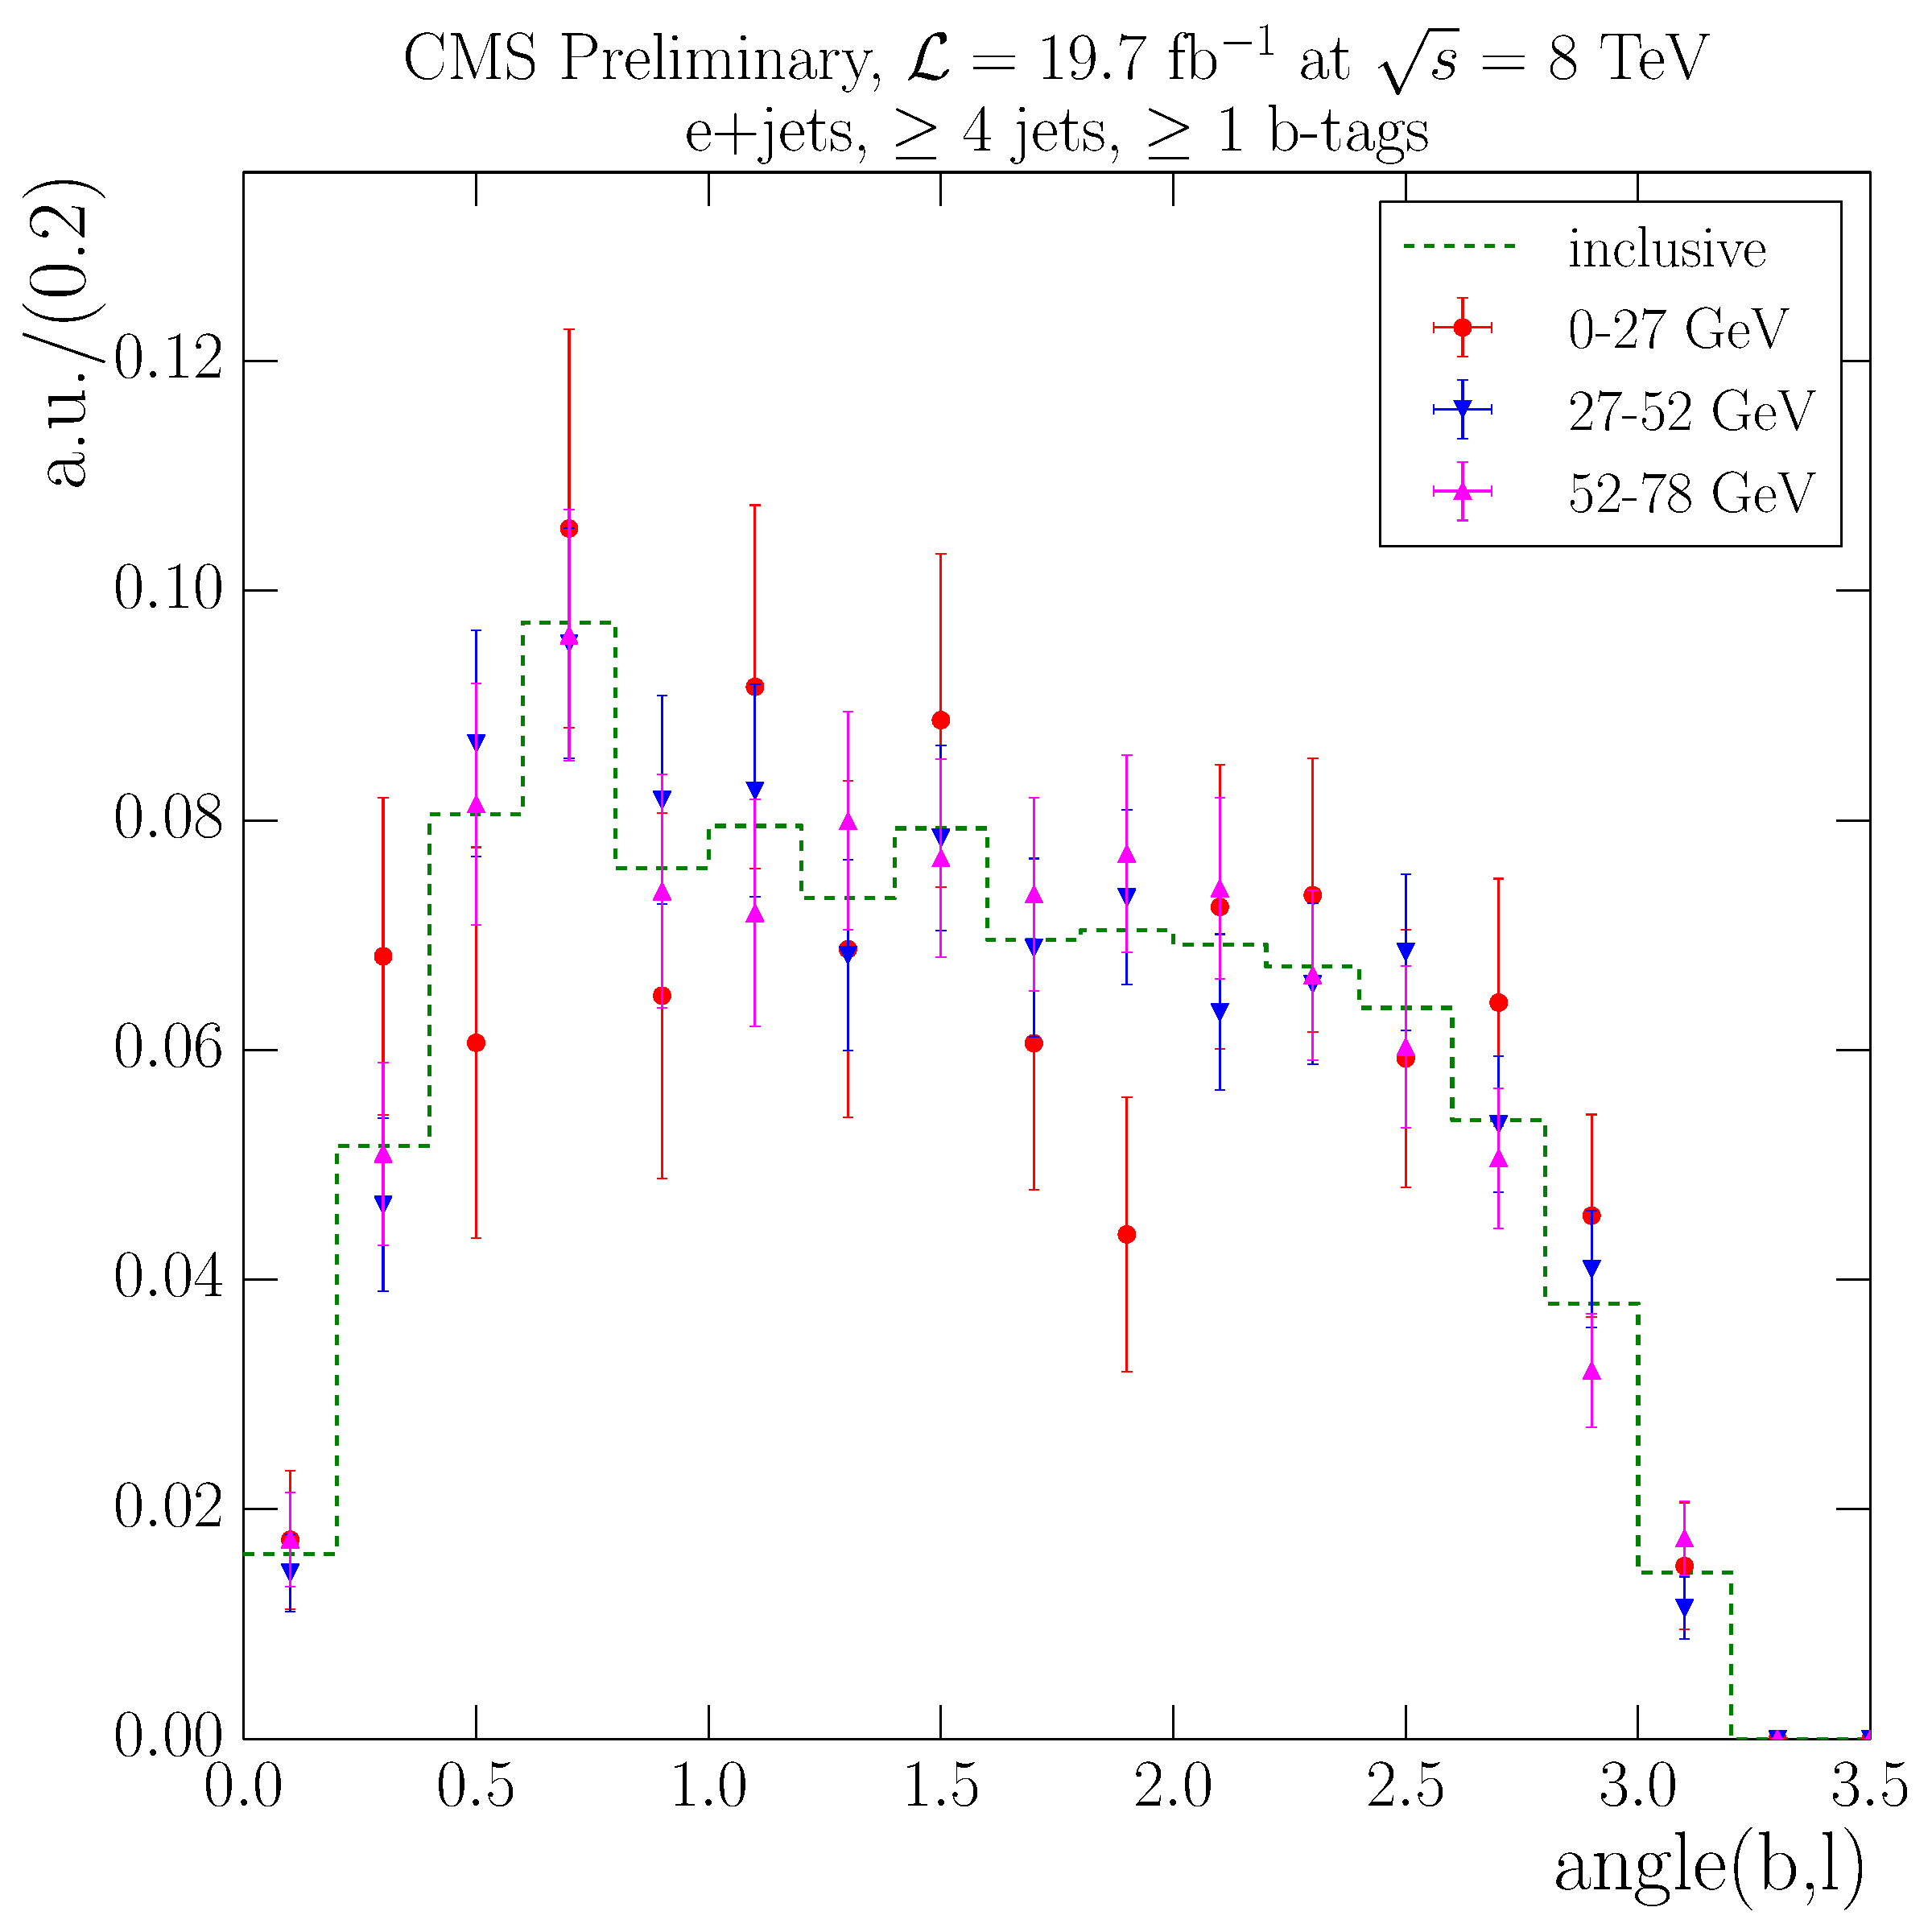
\includegraphics[width=0.48\textwidth]{Chapters/04_Analysis/04b_XSections/images/8TeV/fit_variables/WPT/angle_bl/qcd/WPT_angle_bl_1orMoreBtag_QCD_template_comparison.pdf}\hfill
     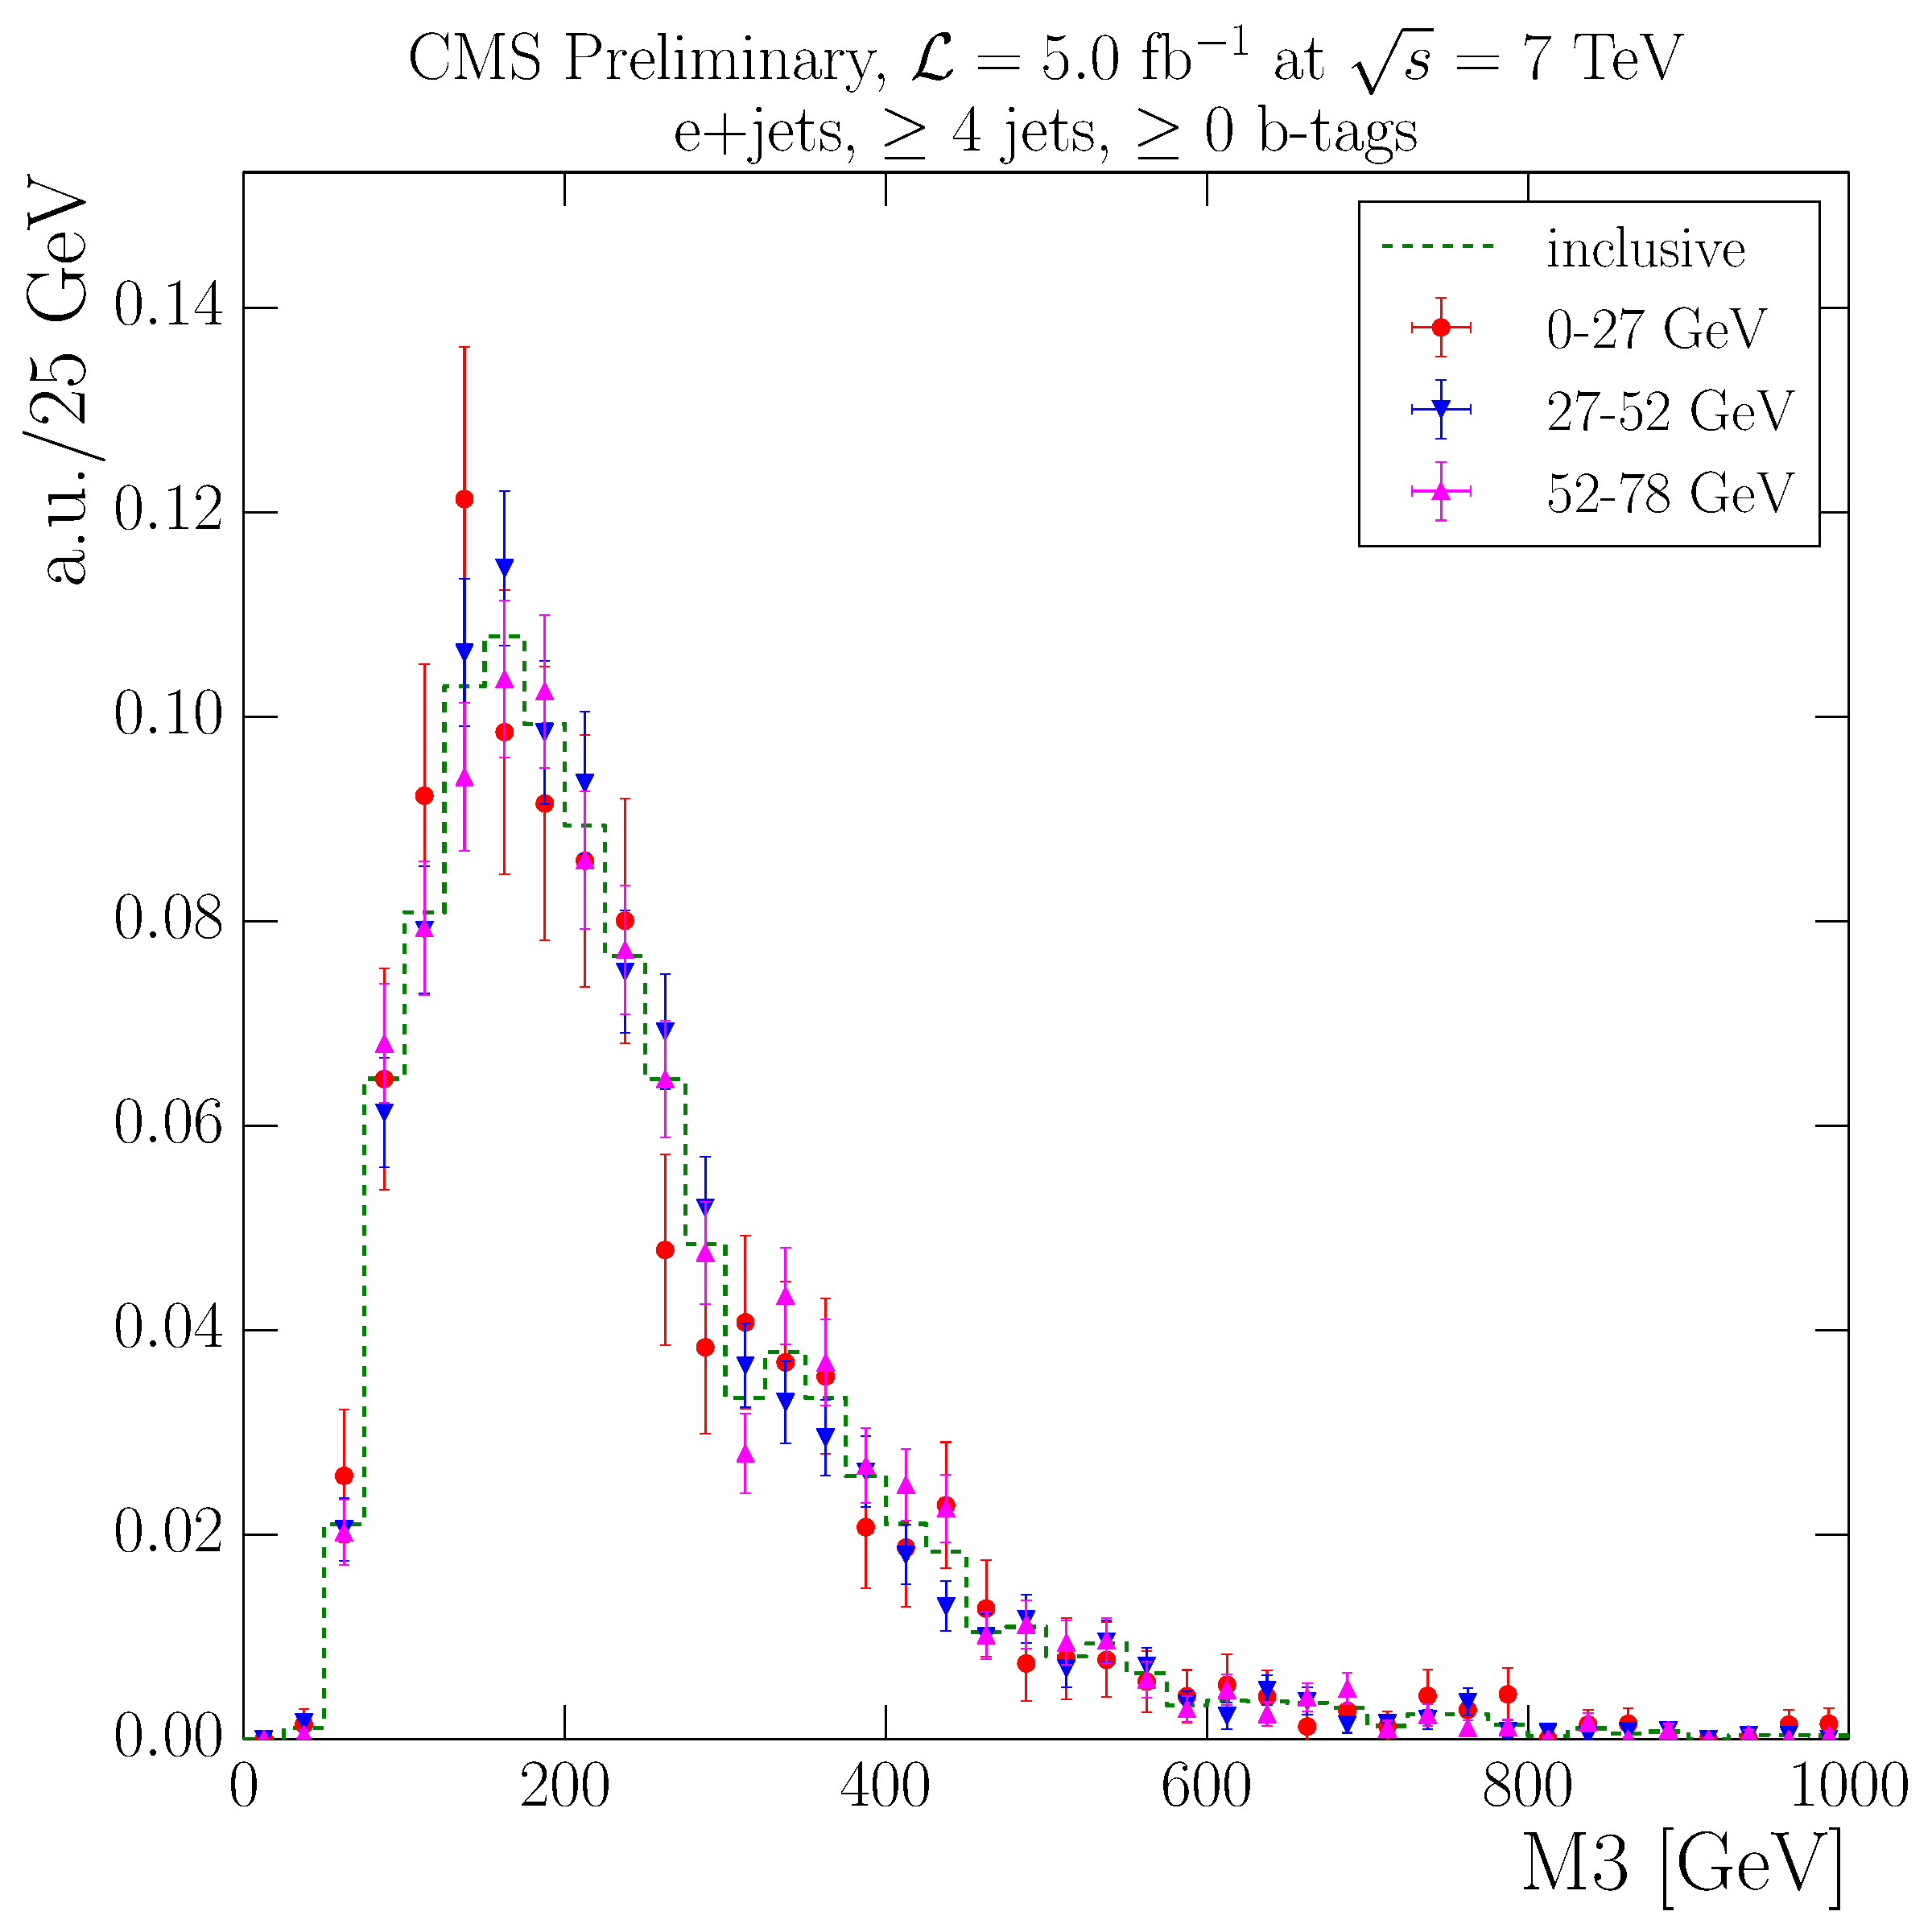
\includegraphics[width=0.48\textwidth]{Chapters/04_Analysis/04b_XSections/images/8TeV/fit_variables/WPT/M3/qcd/WPT_M3_0orMoreBtag_QCD_template_comparison.pdf}\\
	 \caption{Normalised distributions of the QCD templates for the three fit variables at $\sqrt{s}=8\TeV$
	 inclusive across all \wpt bins and for the lowest three \wpt bins: electron \abseta (upper
	 left), muon \abseta (upper right), $\alpha$ (lower left) and M3 (lower right).}
     \label{fig:WPT_fit_variable_qcd_comparisons_8TeV}
\end{figure}


~\section*{Fitting variable V+jets background template comparisons}
\label{as:fitting_variable_vjets_template_comparisons}

\begin{figure}[hbtp]
    \centering
     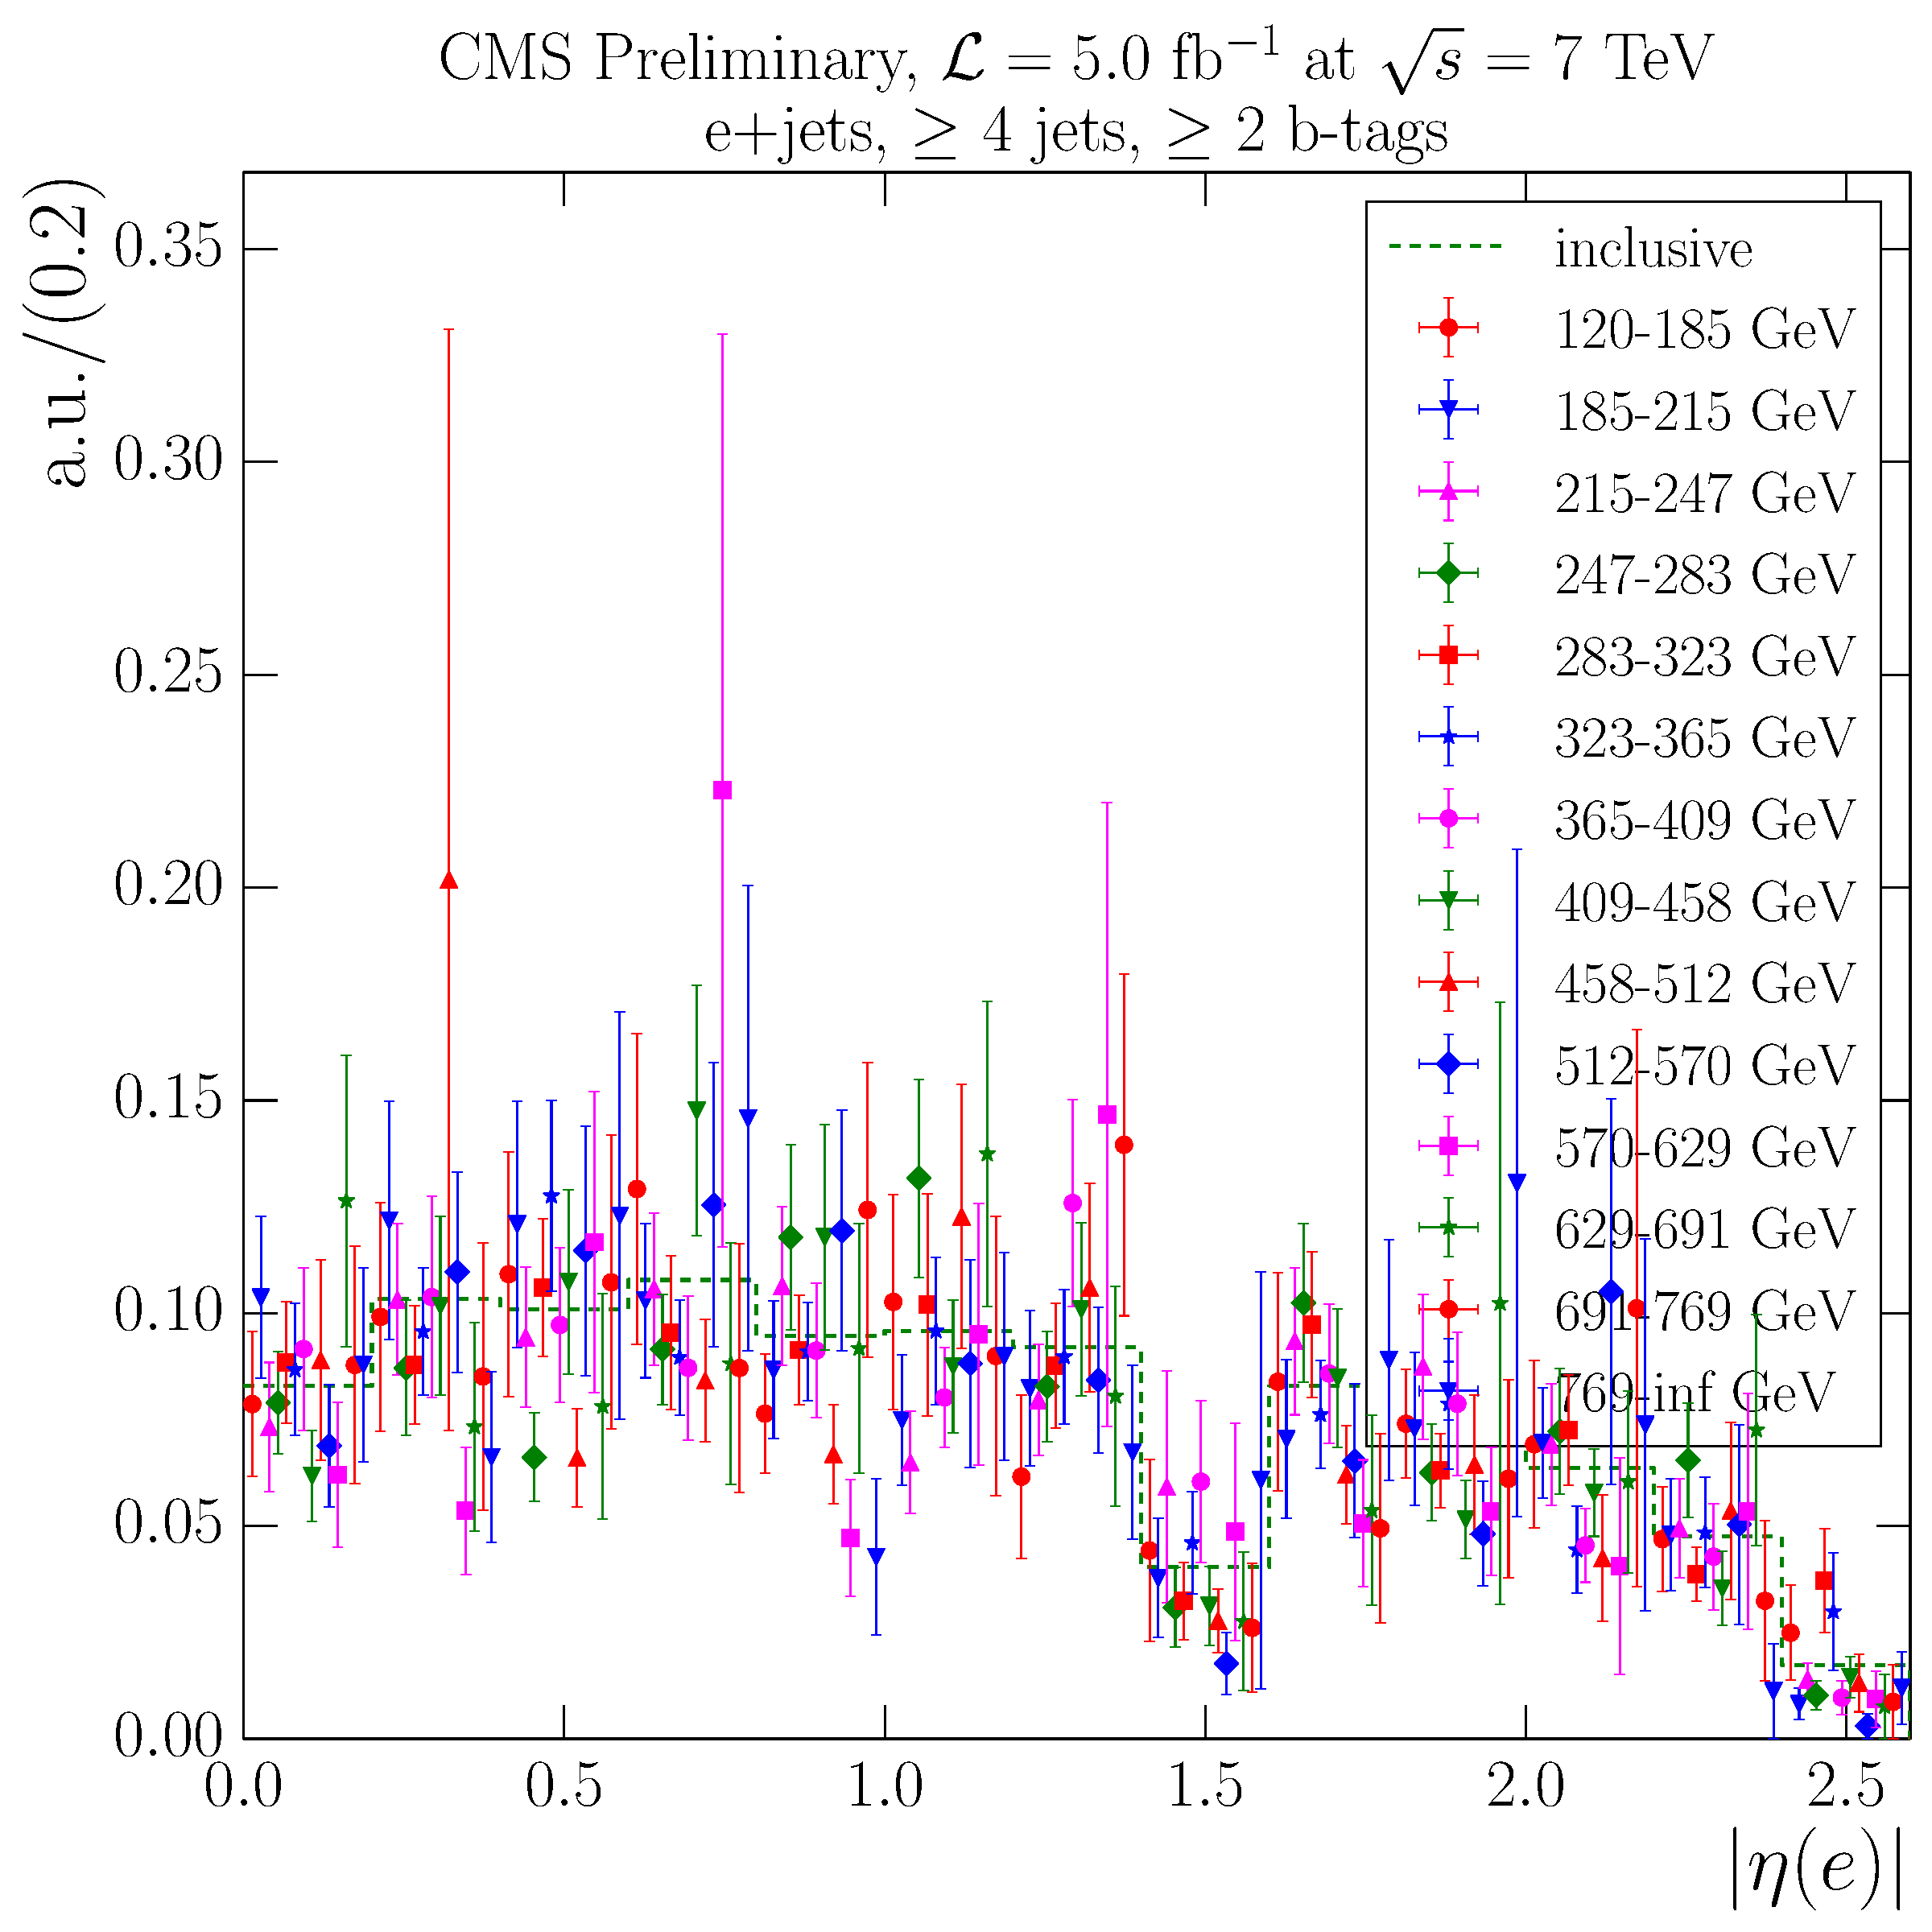
\includegraphics[width=0.48\textwidth]{Chapters/04_Analysis/04b_XSections/images/8TeV/fit_variables/HT/electron_absolute_eta/vjets/HT_electron_absolute_eta_2orMoreBtags_VJets_template_comparison.pdf}\hfill
     
\includegraphics[width=0.48\textwidth]{Chapters/04_Analysis/04b_XSections/images/placeholder.png}\\
     %\includegraphics[width=0.48\textwidth]{Chapters/04_Analysis/04b_XSections/images/7TeV/fit_variables/HT/muon_absolute_eta/vjets/HT_inclusive_muon_absolute_eta_2orMoreBtags_templates.pdf}\\    
     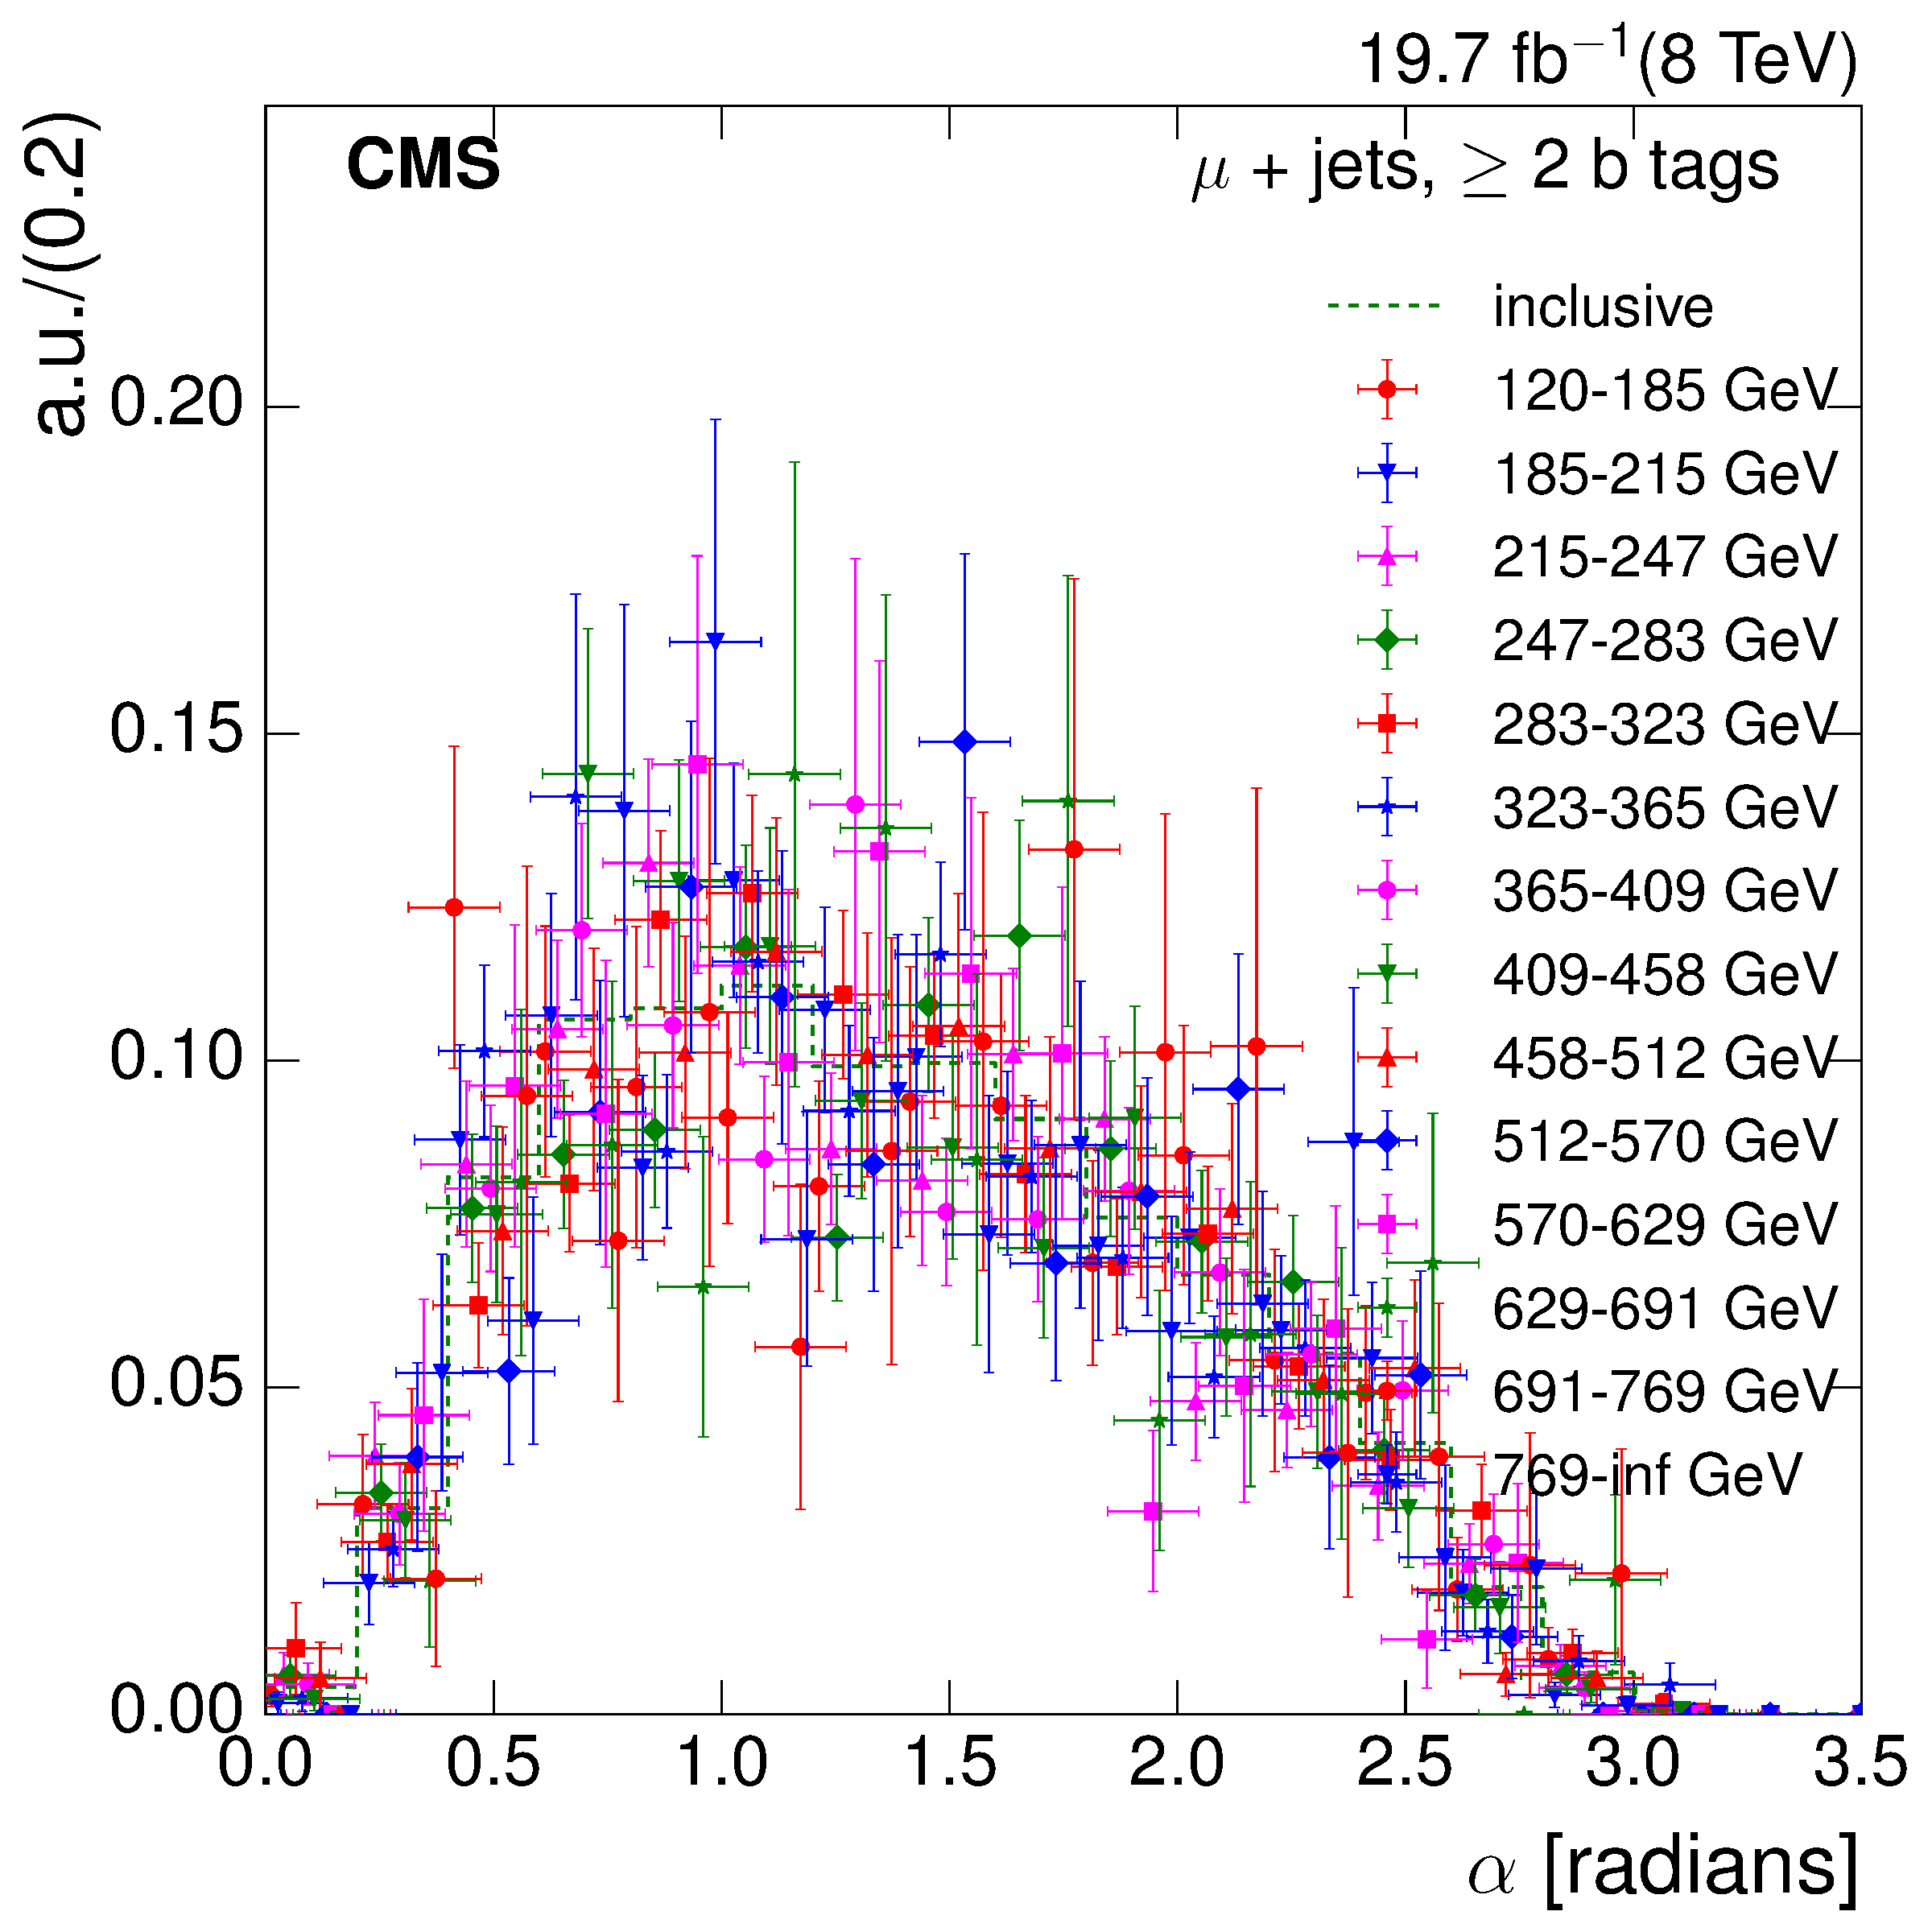
\includegraphics[width=0.48\textwidth]{Chapters/04_Analysis/04b_XSections/images/8TeV/fit_variables/HT/angle_bl/vjets/HT_angle_bl_2orMoreBtags_VJets_template_comparison.pdf}\hfill
     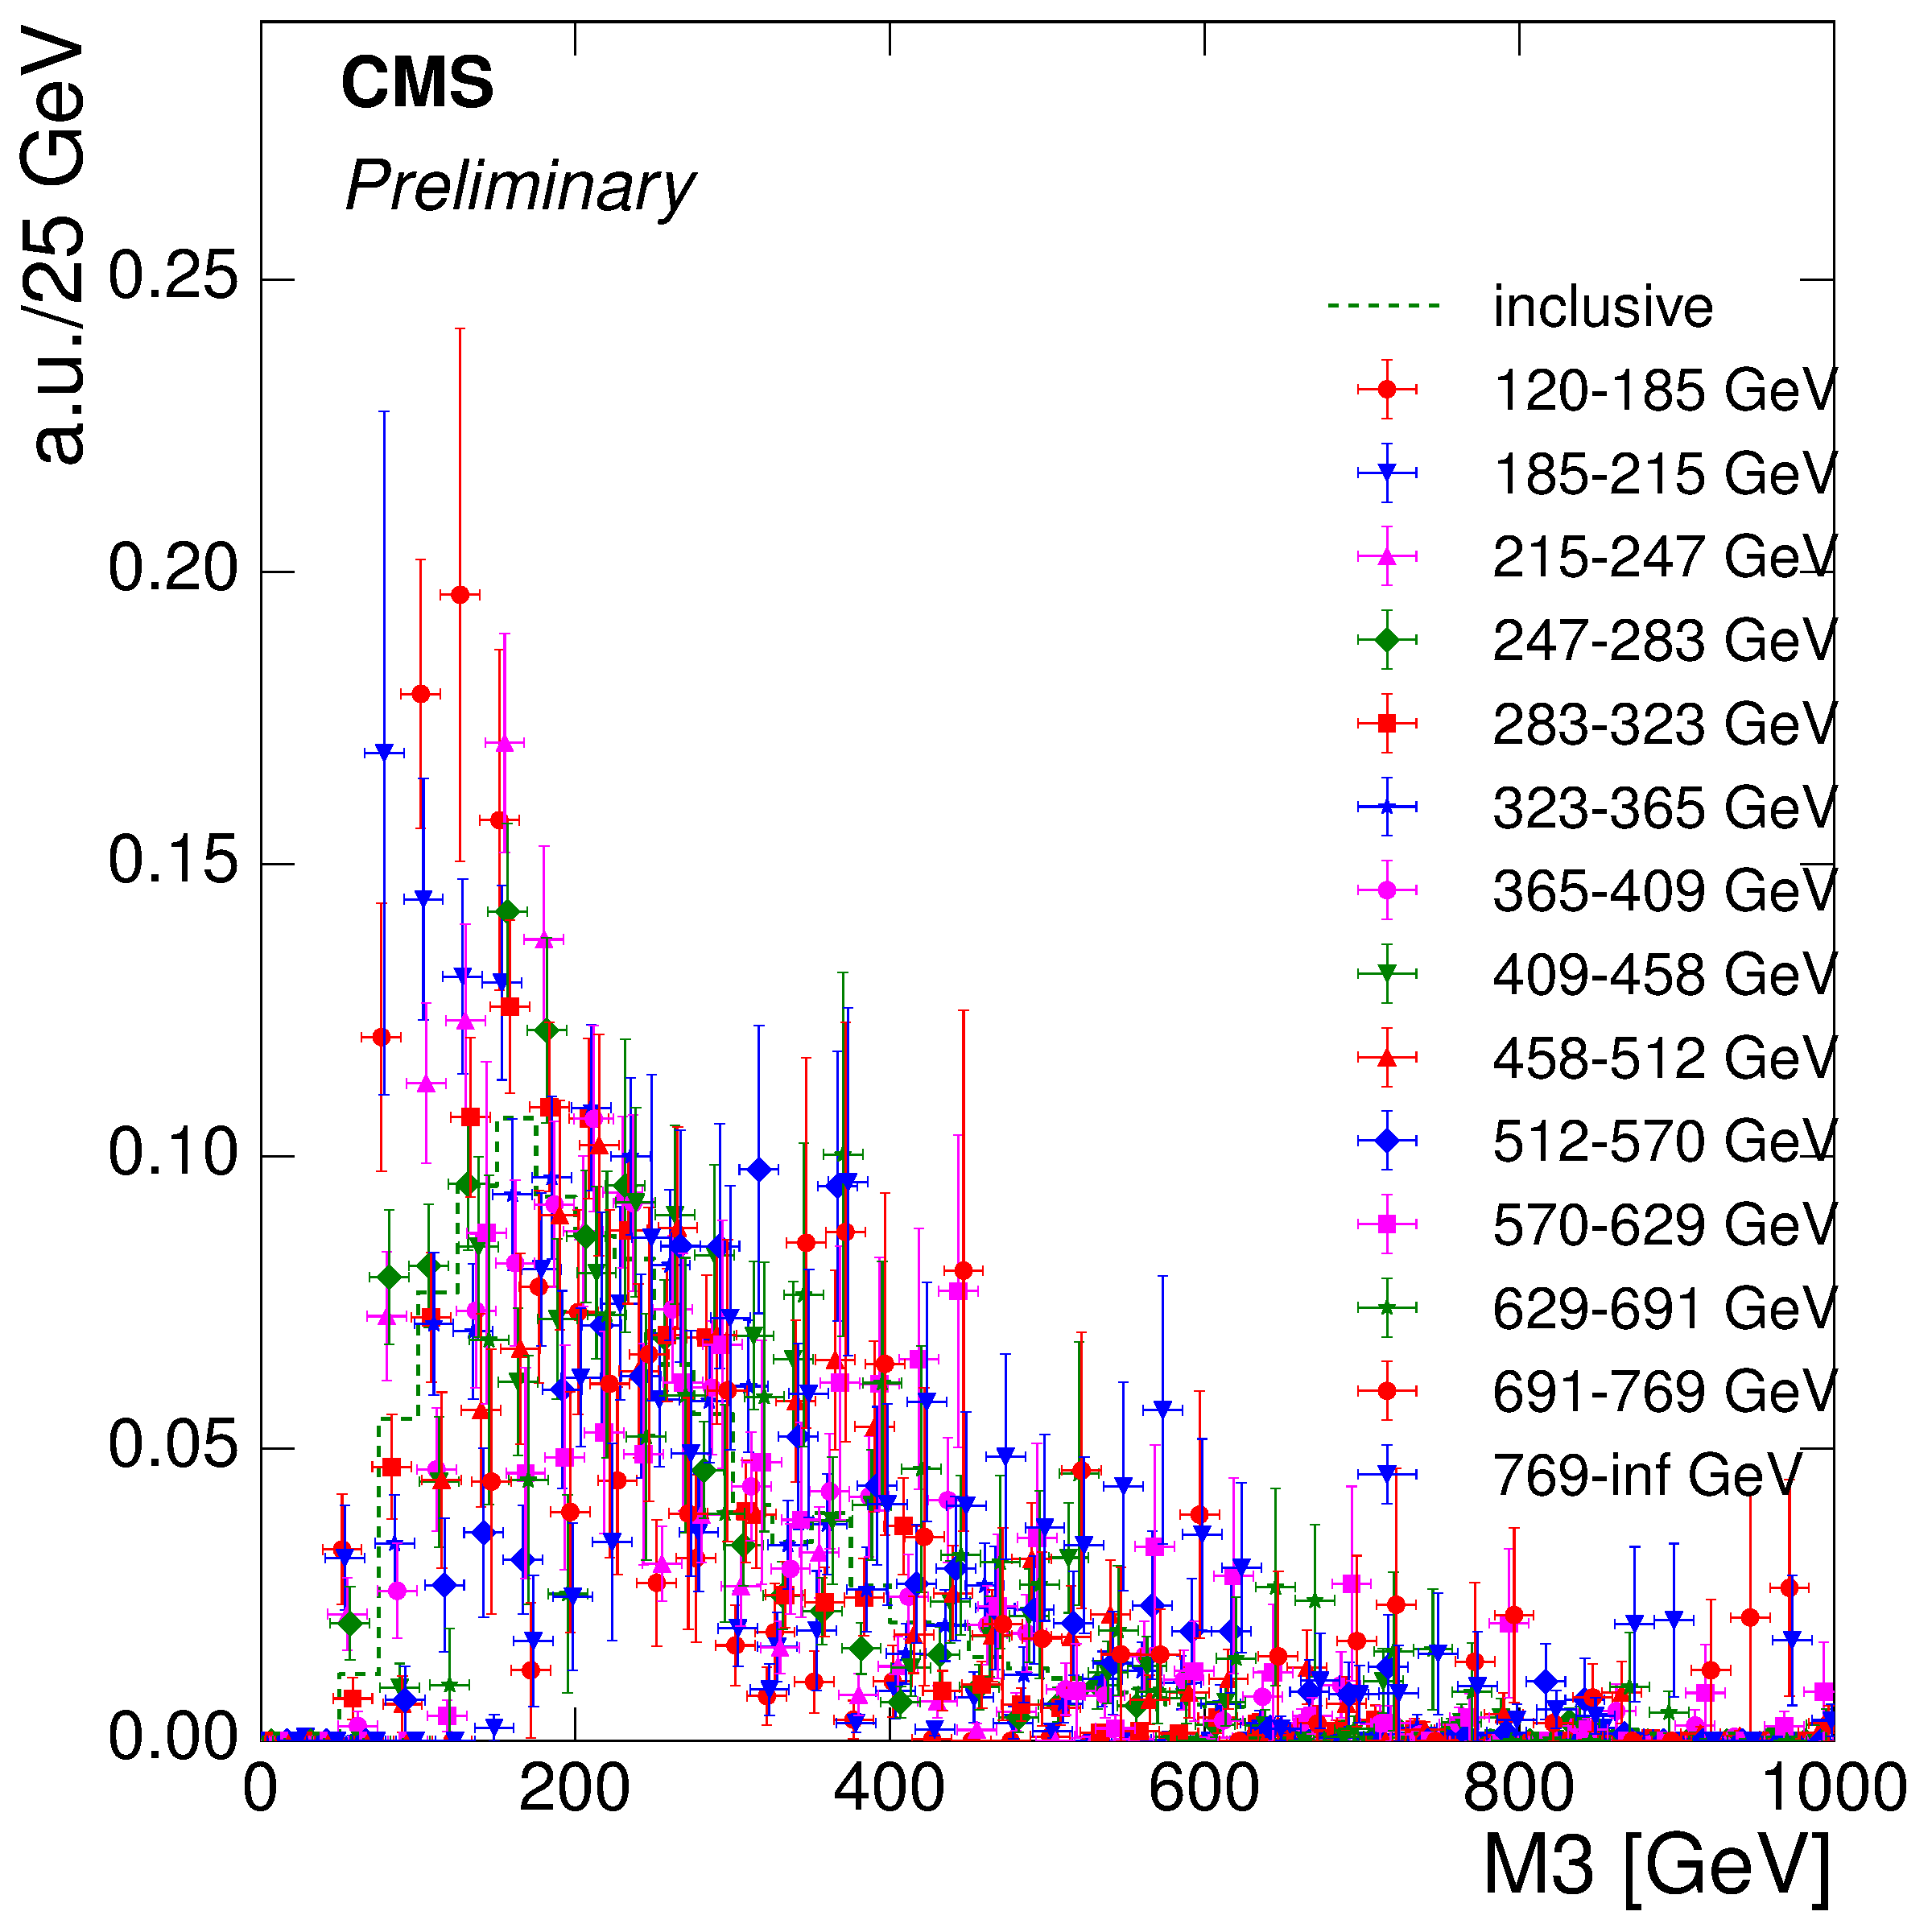
\includegraphics[width=0.48\textwidth]{Chapters/04_Analysis/04b_XSections/images/8TeV/fit_variables/HT/M3/vjets/HT_M3_2orMoreBtags_VJets_template_comparison.pdf}\\
	 \caption{Normalised distributions of the V+jets templates for the three fit variables at $\sqrt{s}=8\TeV$
	 inclusive across all \HT bins and for individual \HT bins: electron \abseta (upper
	 left), muon \abseta (upper right), $\alpha$ (lower left) and M3 (lower right).}
     \label{fig:HT_fit_variable_vjets_comparisons_8TeV}
\end{figure}

\begin{figure}[hbtp]
    \centering
     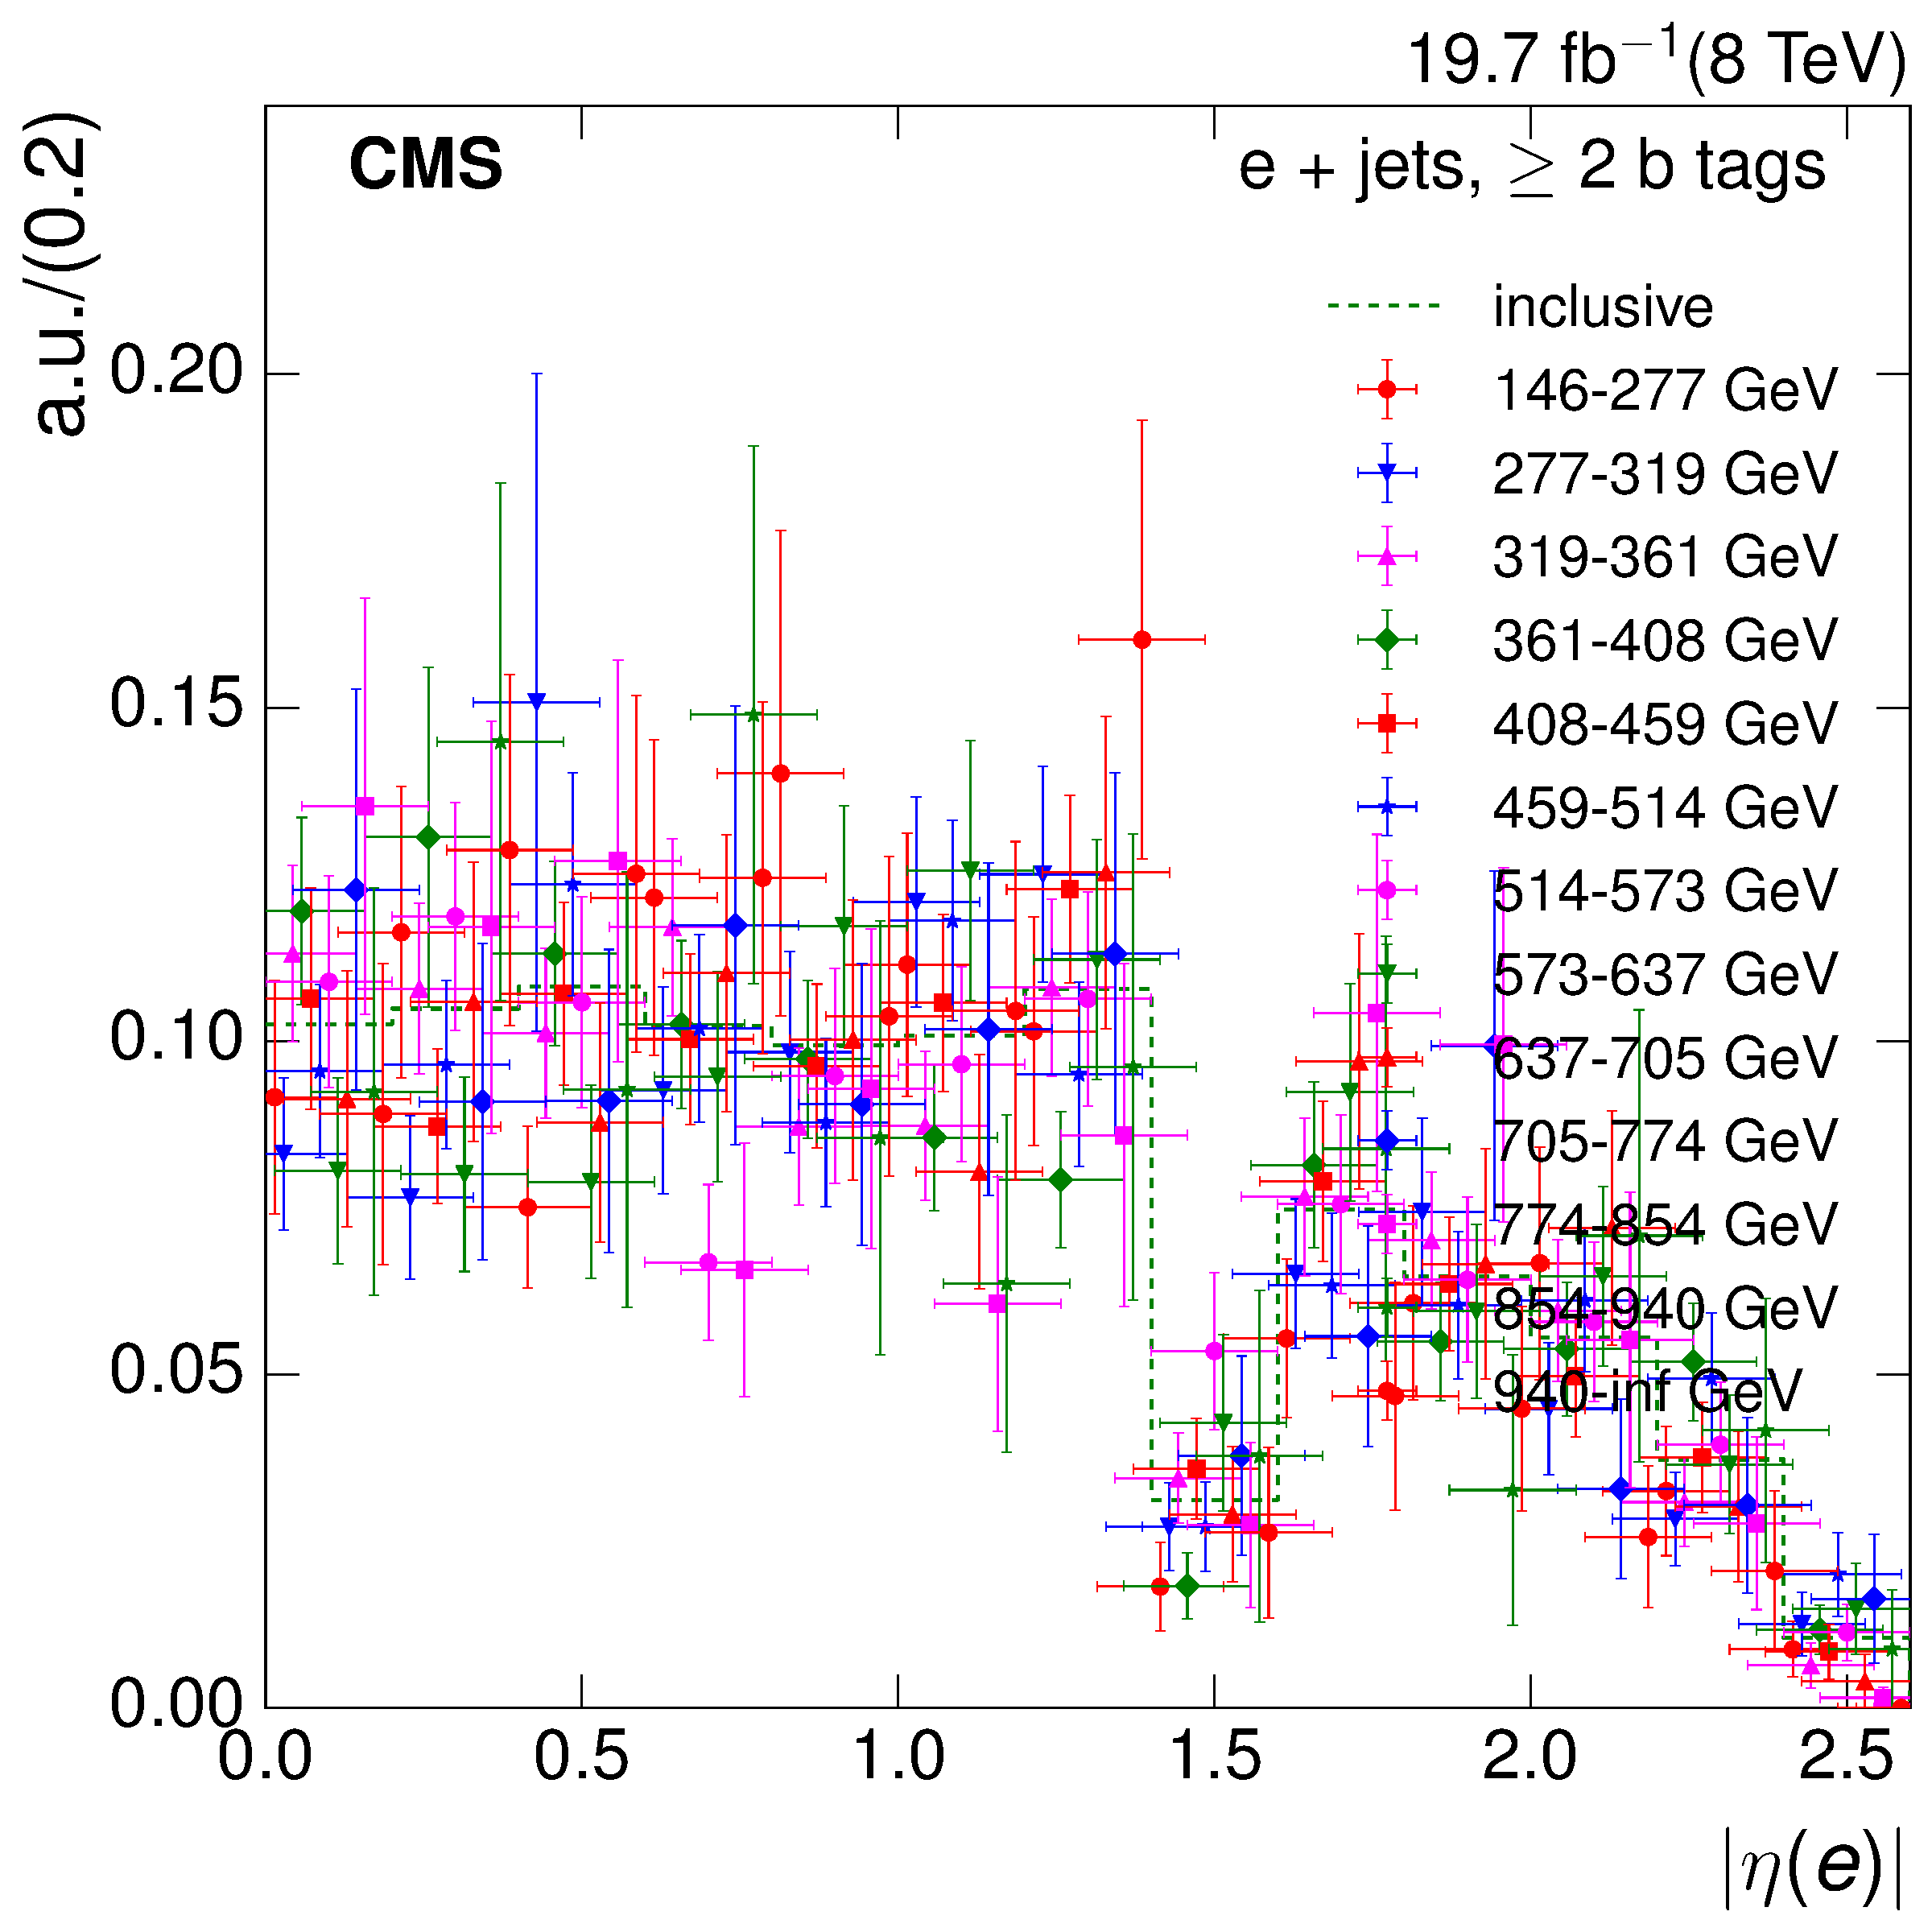
\includegraphics[width=0.48\textwidth]{Chapters/04_Analysis/04b_XSections/images/8TeV/fit_variables/ST/electron_absolute_eta/vjets/ST_electron_absolute_eta_2orMoreBtags_VJets_template_comparison.pdf}\hfill
     
\includegraphics[width=0.48\textwidth]{Chapters/04_Analysis/04b_XSections/images/placeholder.png}\\
     %\includegraphics[width=0.48\textwidth]{Chapters/04_Analysis/04b_XSections/images/7TeV/fit_variables/ST/muon_absolute_eta/vjets/ST_inclusive_muon_absolute_eta_2orMoreBtags_templates.pdf}\\    
     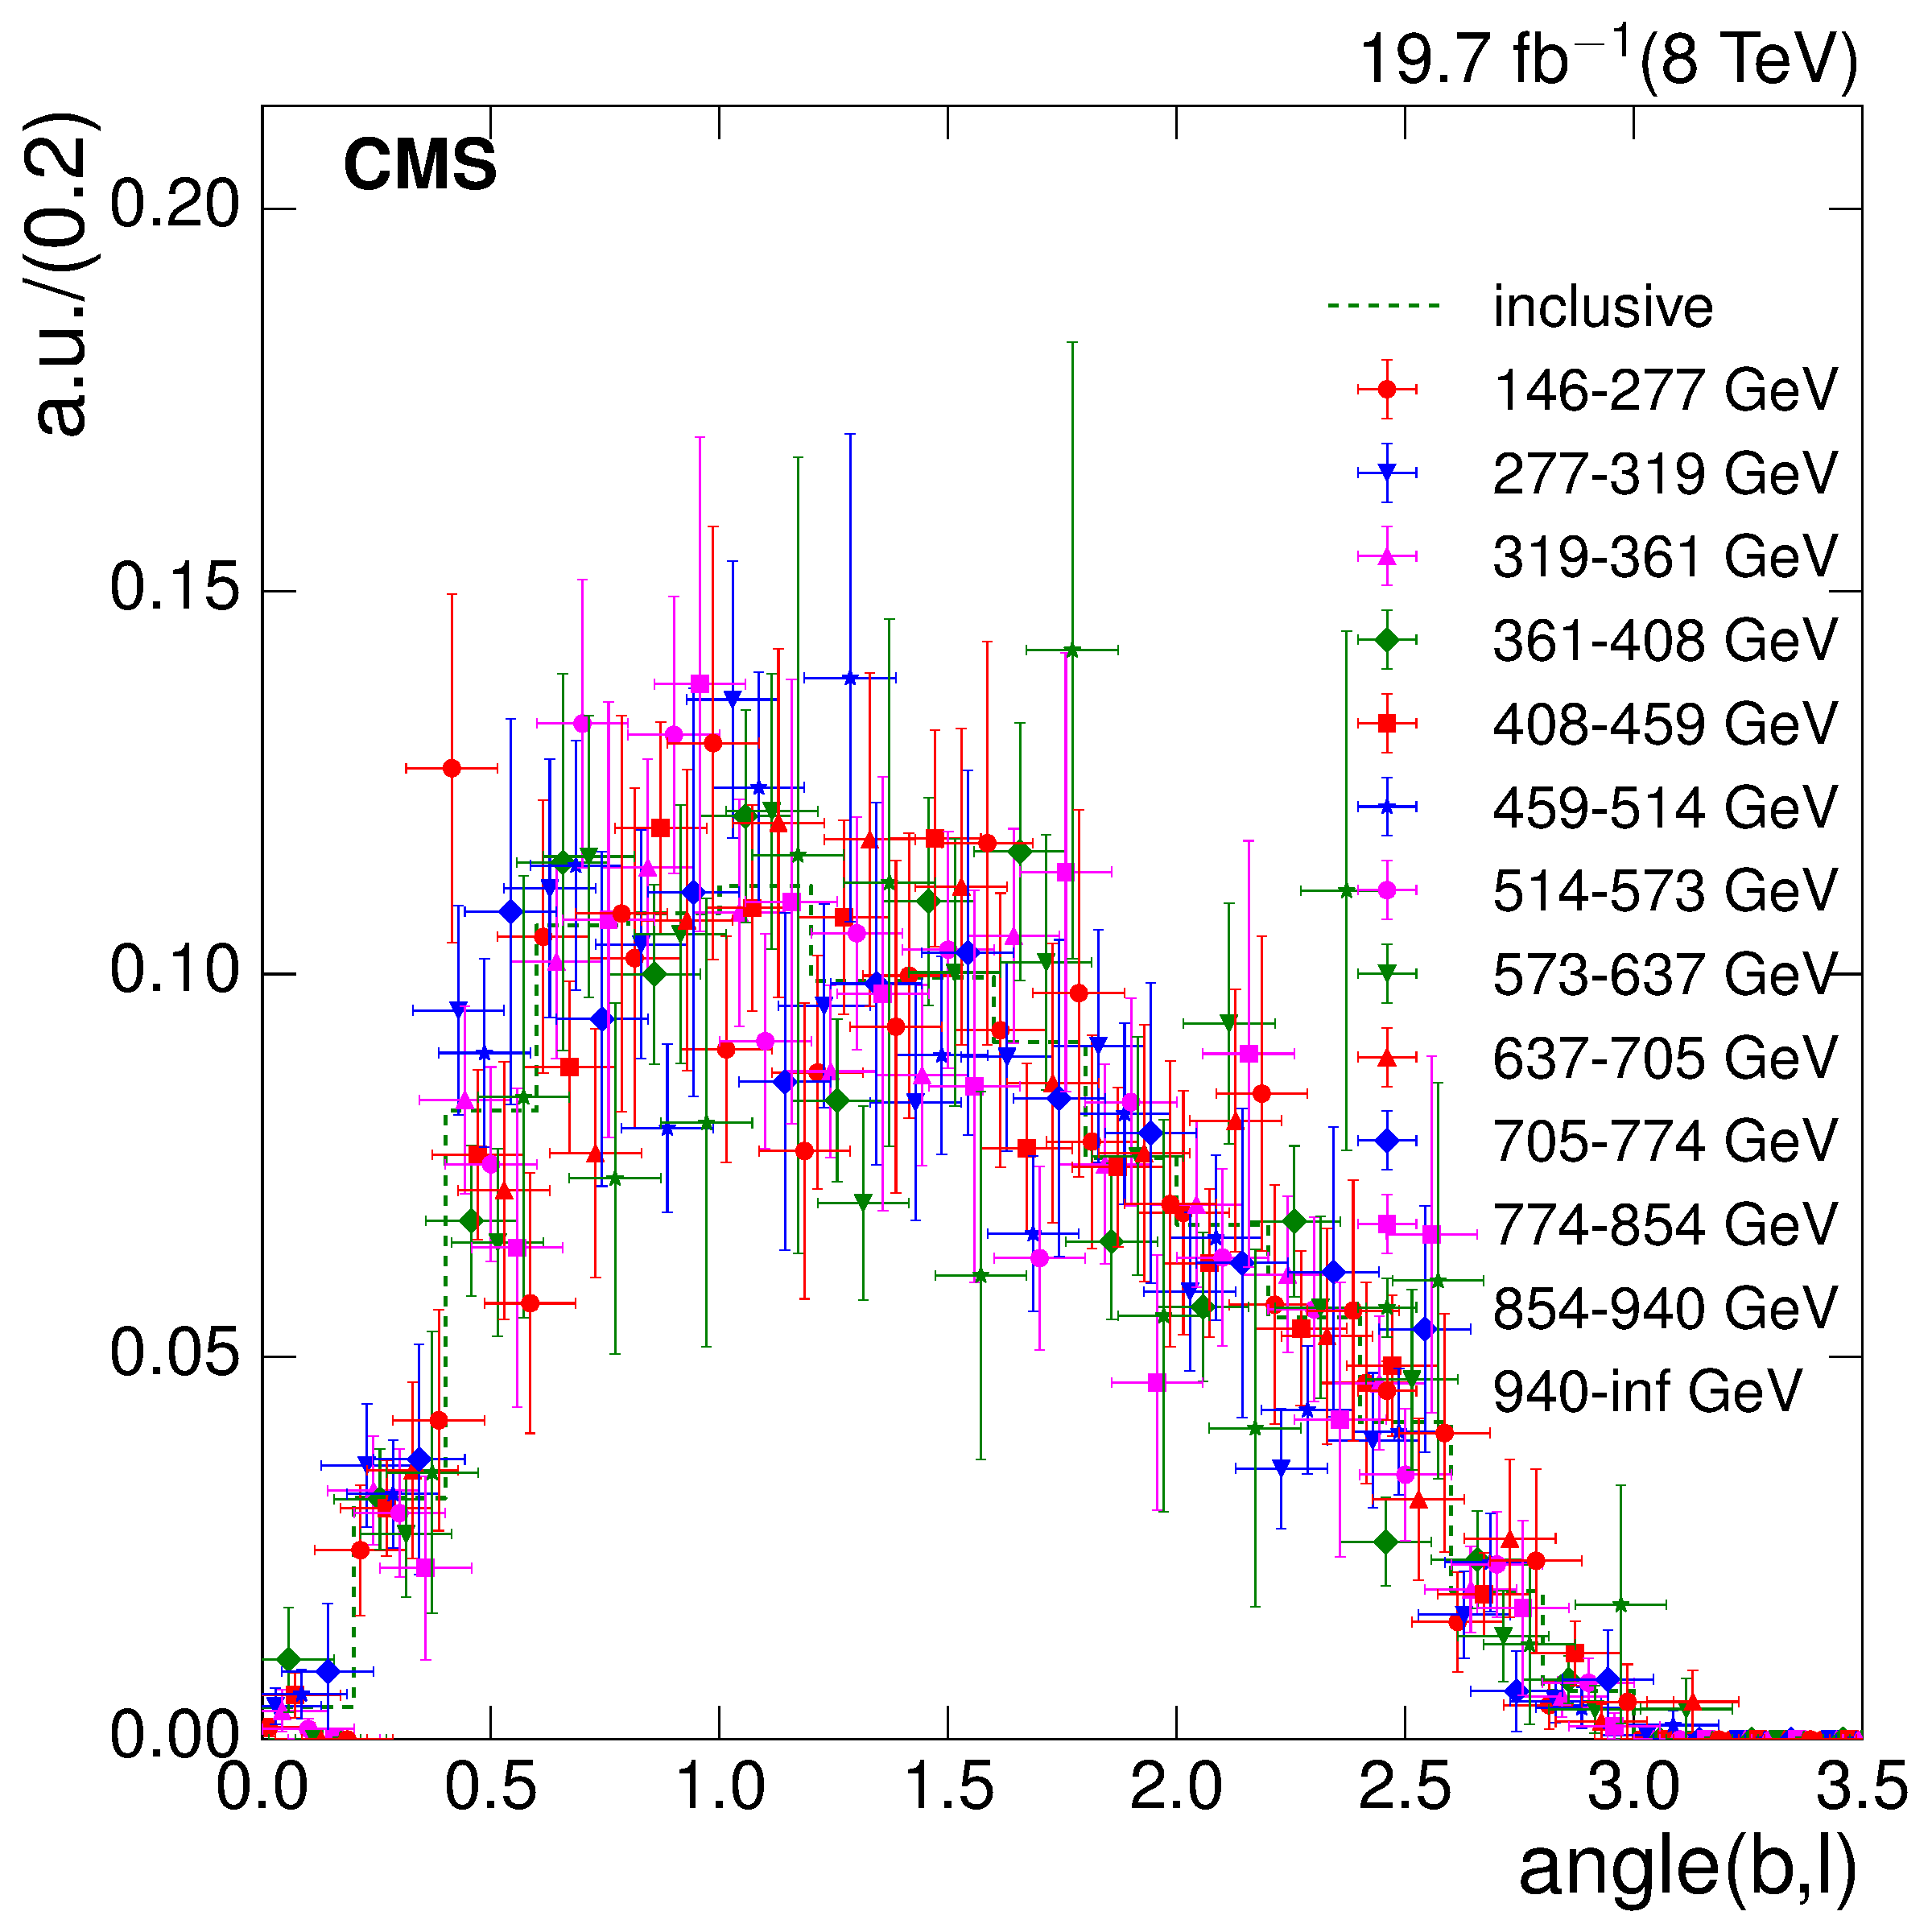
\includegraphics[width=0.48\textwidth]{Chapters/04_Analysis/04b_XSections/images/8TeV/fit_variables/ST/angle_bl/vjets/ST_angle_bl_2orMoreBtags_VJets_template_comparison.pdf}\hfill
     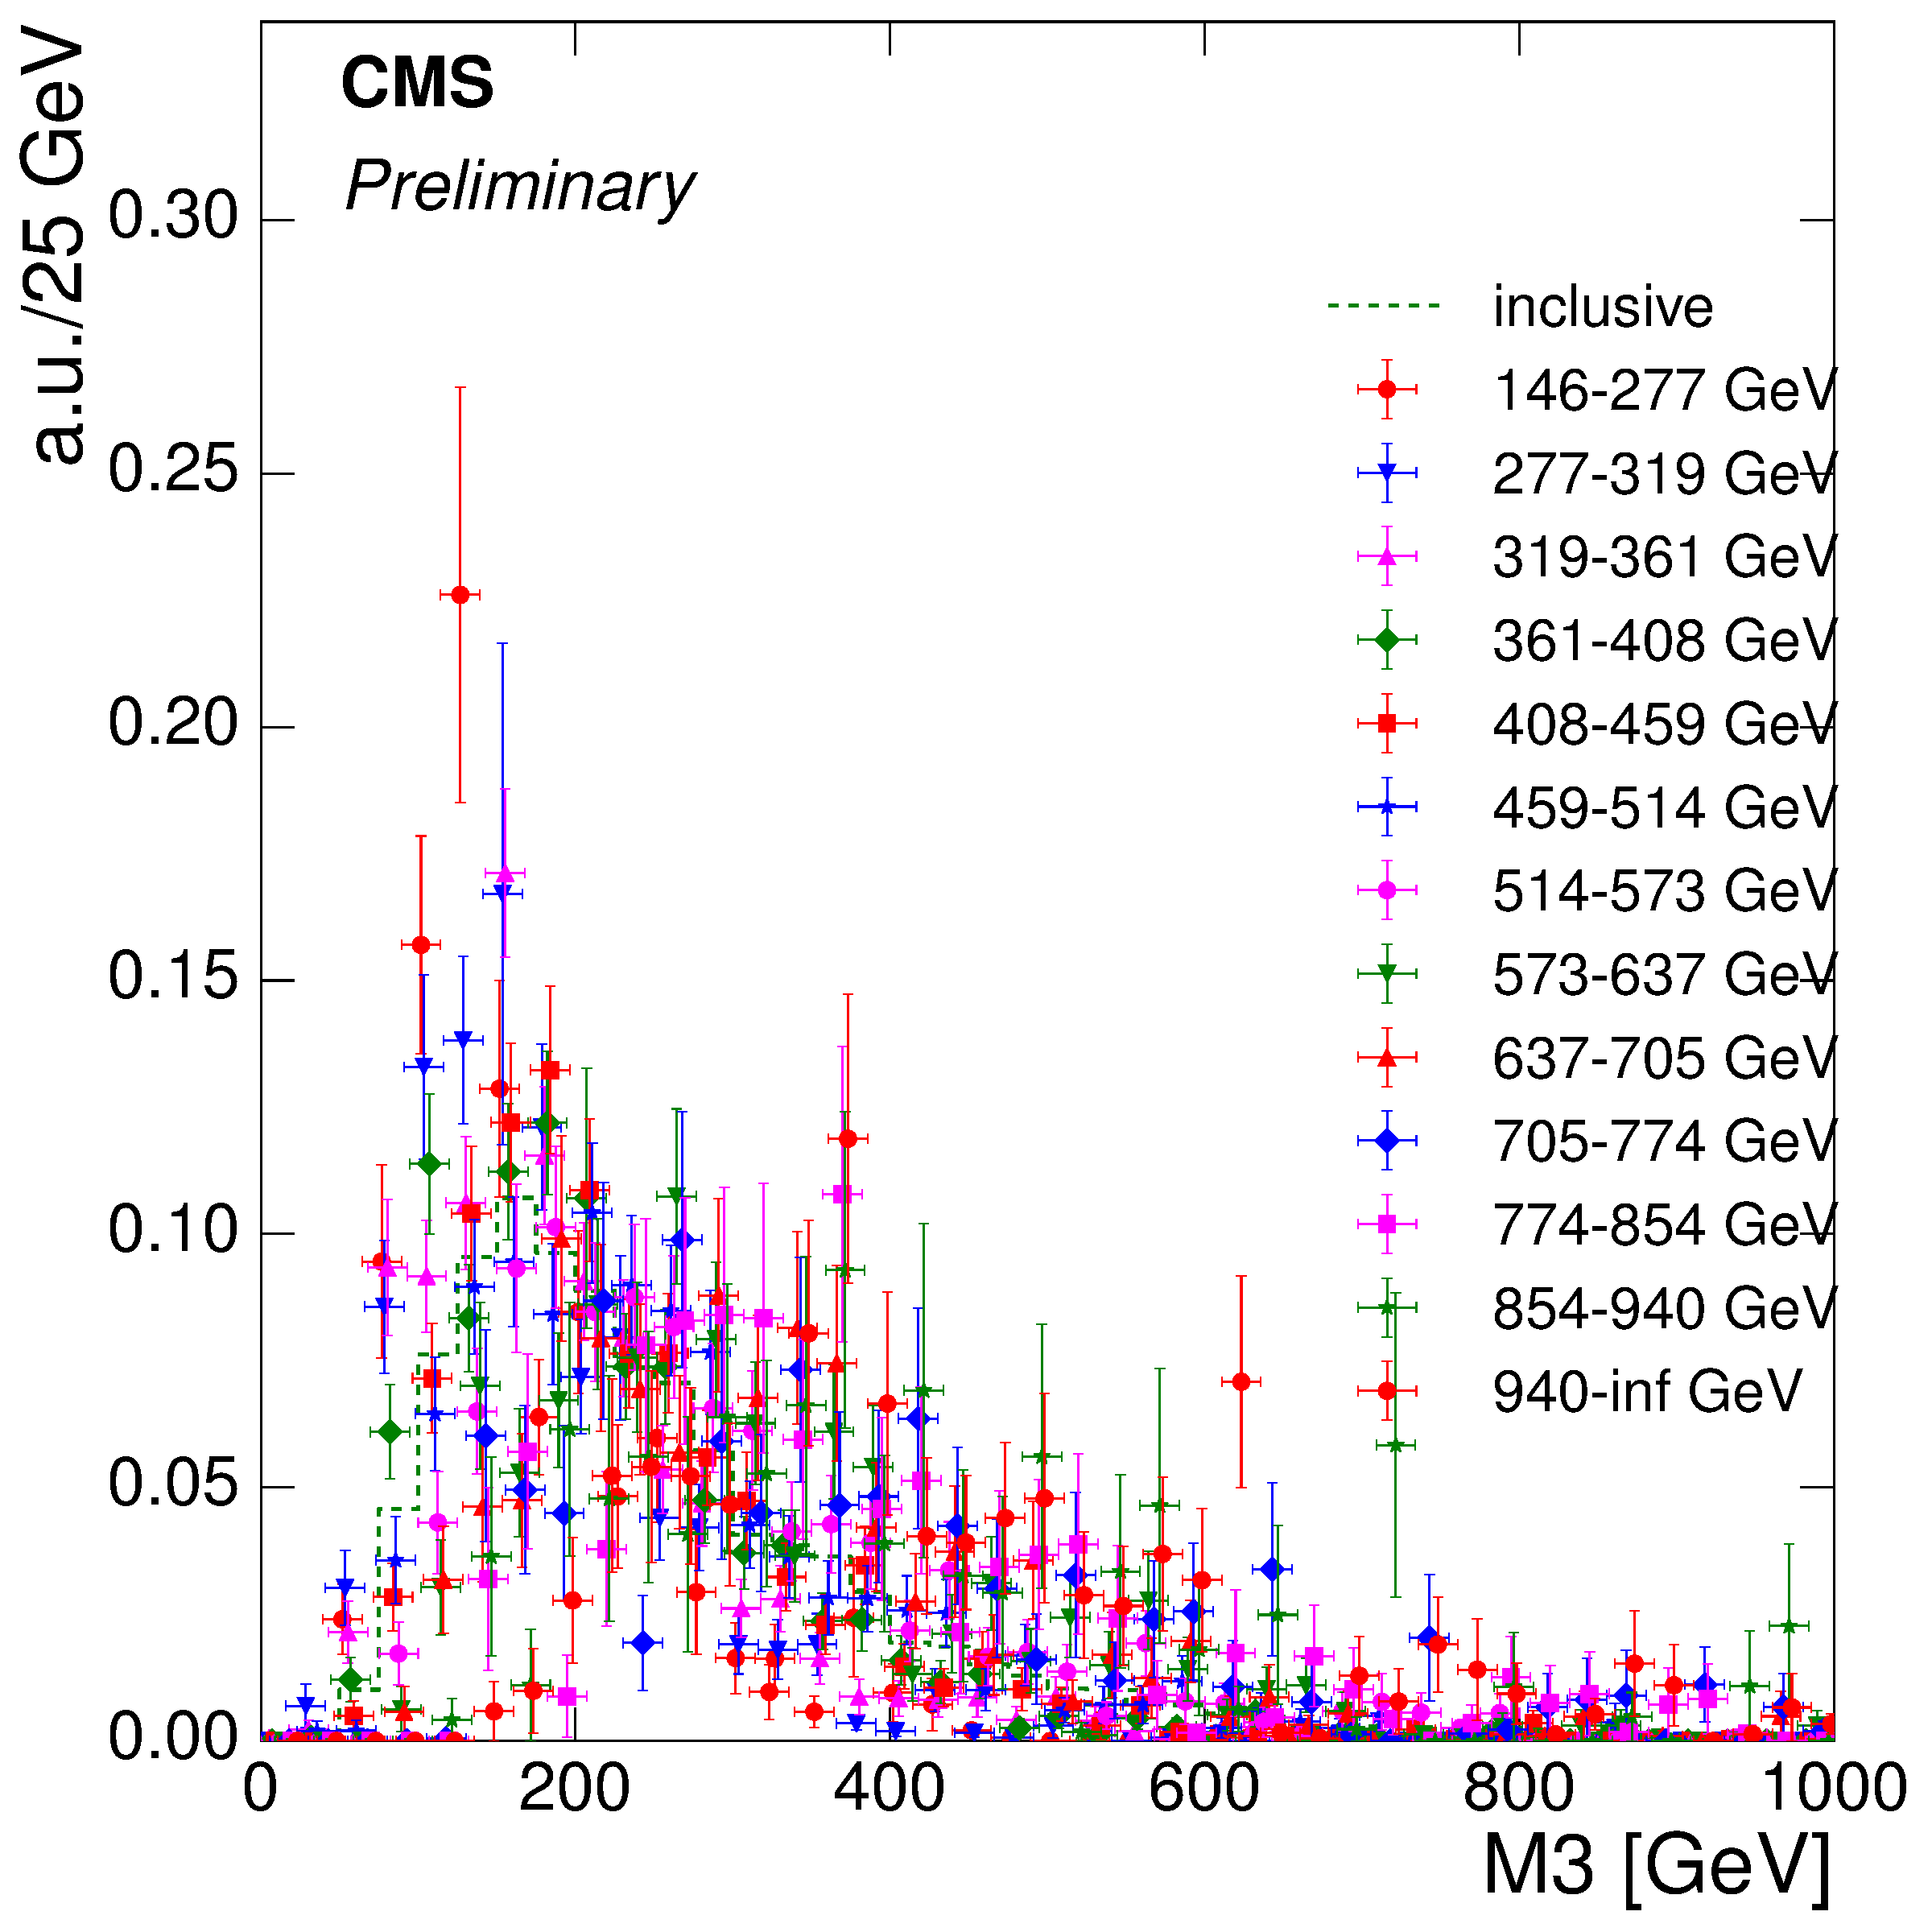
\includegraphics[width=0.48\textwidth]{Chapters/04_Analysis/04b_XSections/images/8TeV/fit_variables/ST/M3/vjets/ST_M3_2orMoreBtags_VJets_template_comparison.pdf}\\
	 \caption{Normalised distributions of the V+jets templates for the three fit variables at $\sqrt{s}=8\TeV$
	 inclusive across all \st bins and for individual \st bins: electron \abseta (upper
	 left), muon \abseta (upper right), $\alpha$ (lower left) and M3 (lower right).}
     \label{fig:ST_fit_variable_vjets_comparisons_8TeV}
\end{figure}

\begin{figure}[hbtp]
    \centering
     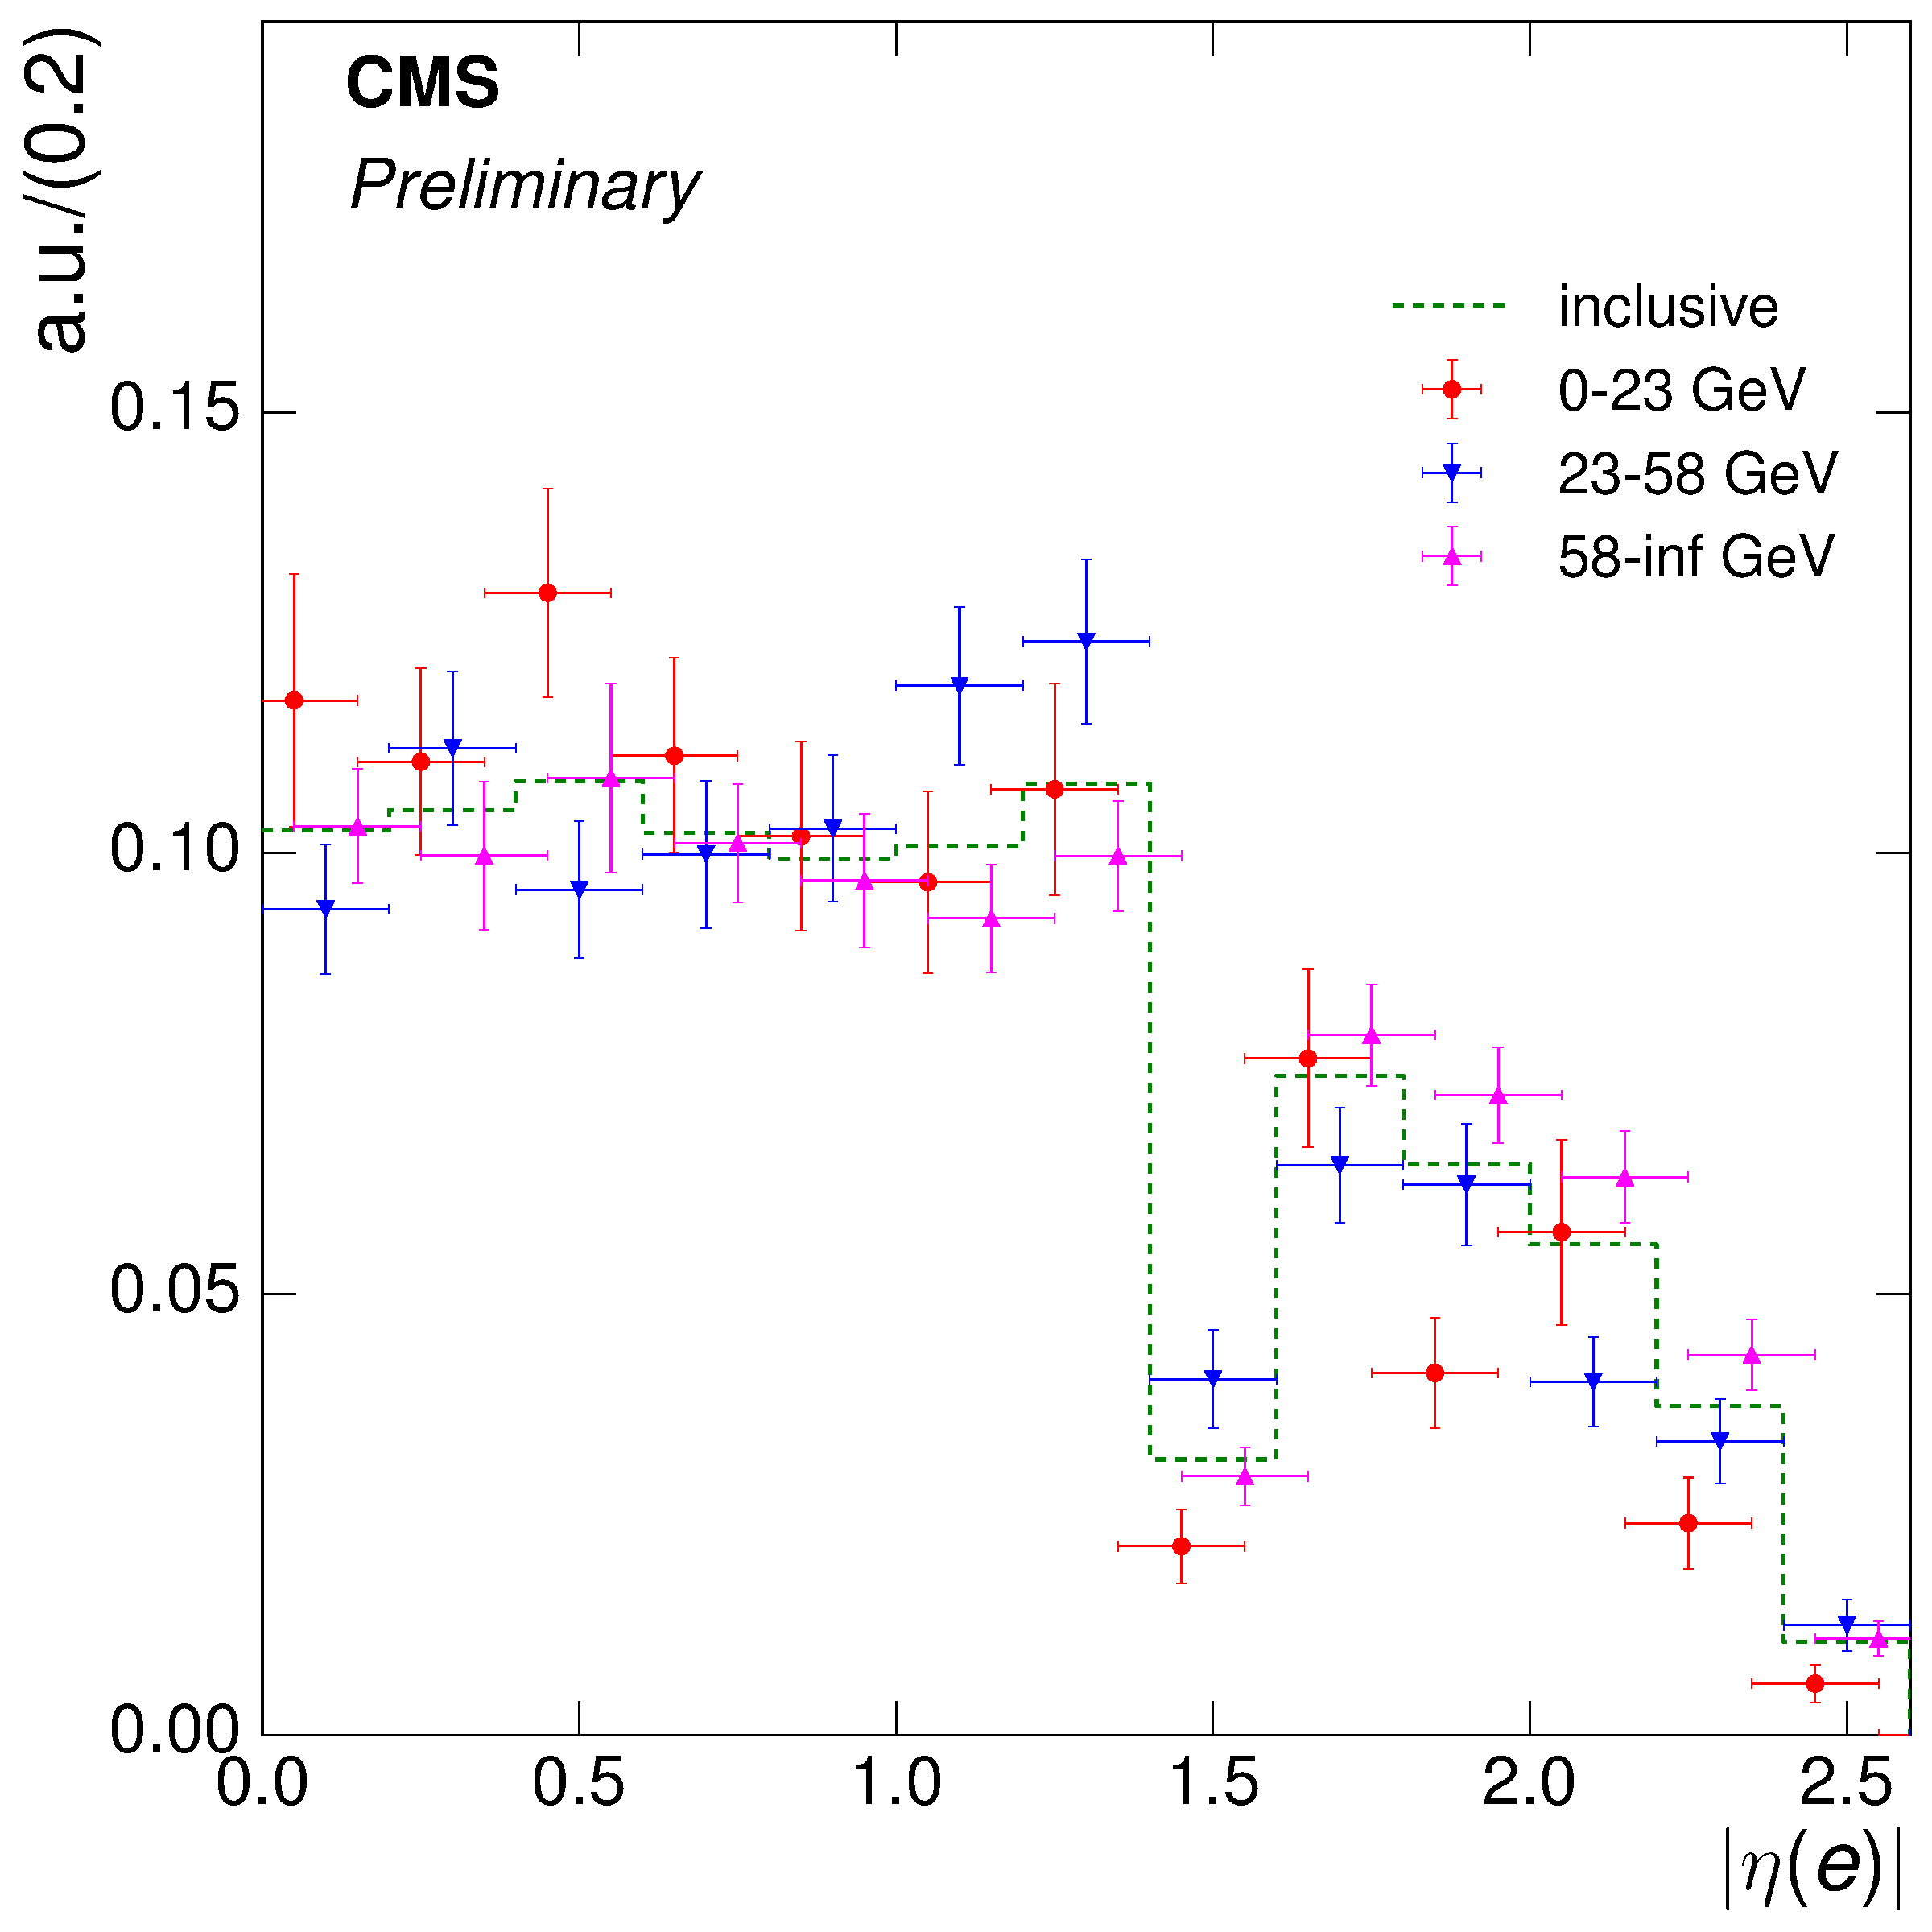
\includegraphics[width=0.48\textwidth]{Chapters/04_Analysis/04b_XSections/images/8TeV/fit_variables/MT/electron_absolute_eta/vjets/MT_electron_absolute_eta_2orMoreBtags_VJets_template_comparison.pdf}\hfill
     
\includegraphics[width=0.48\textwidth]{Chapters/04_Analysis/04b_XSections/images/placeholder.png}\\
     %\includegraphics[width=0.48\textwidth]{Chapters/04_Analysis/04b_XSections/images/7TeV/fit_variables/MT/muon_absolute_eta/vjets/MT_inclusive_muon_absolute_eta_2orMoreBtags_templates.pdf}\\    
     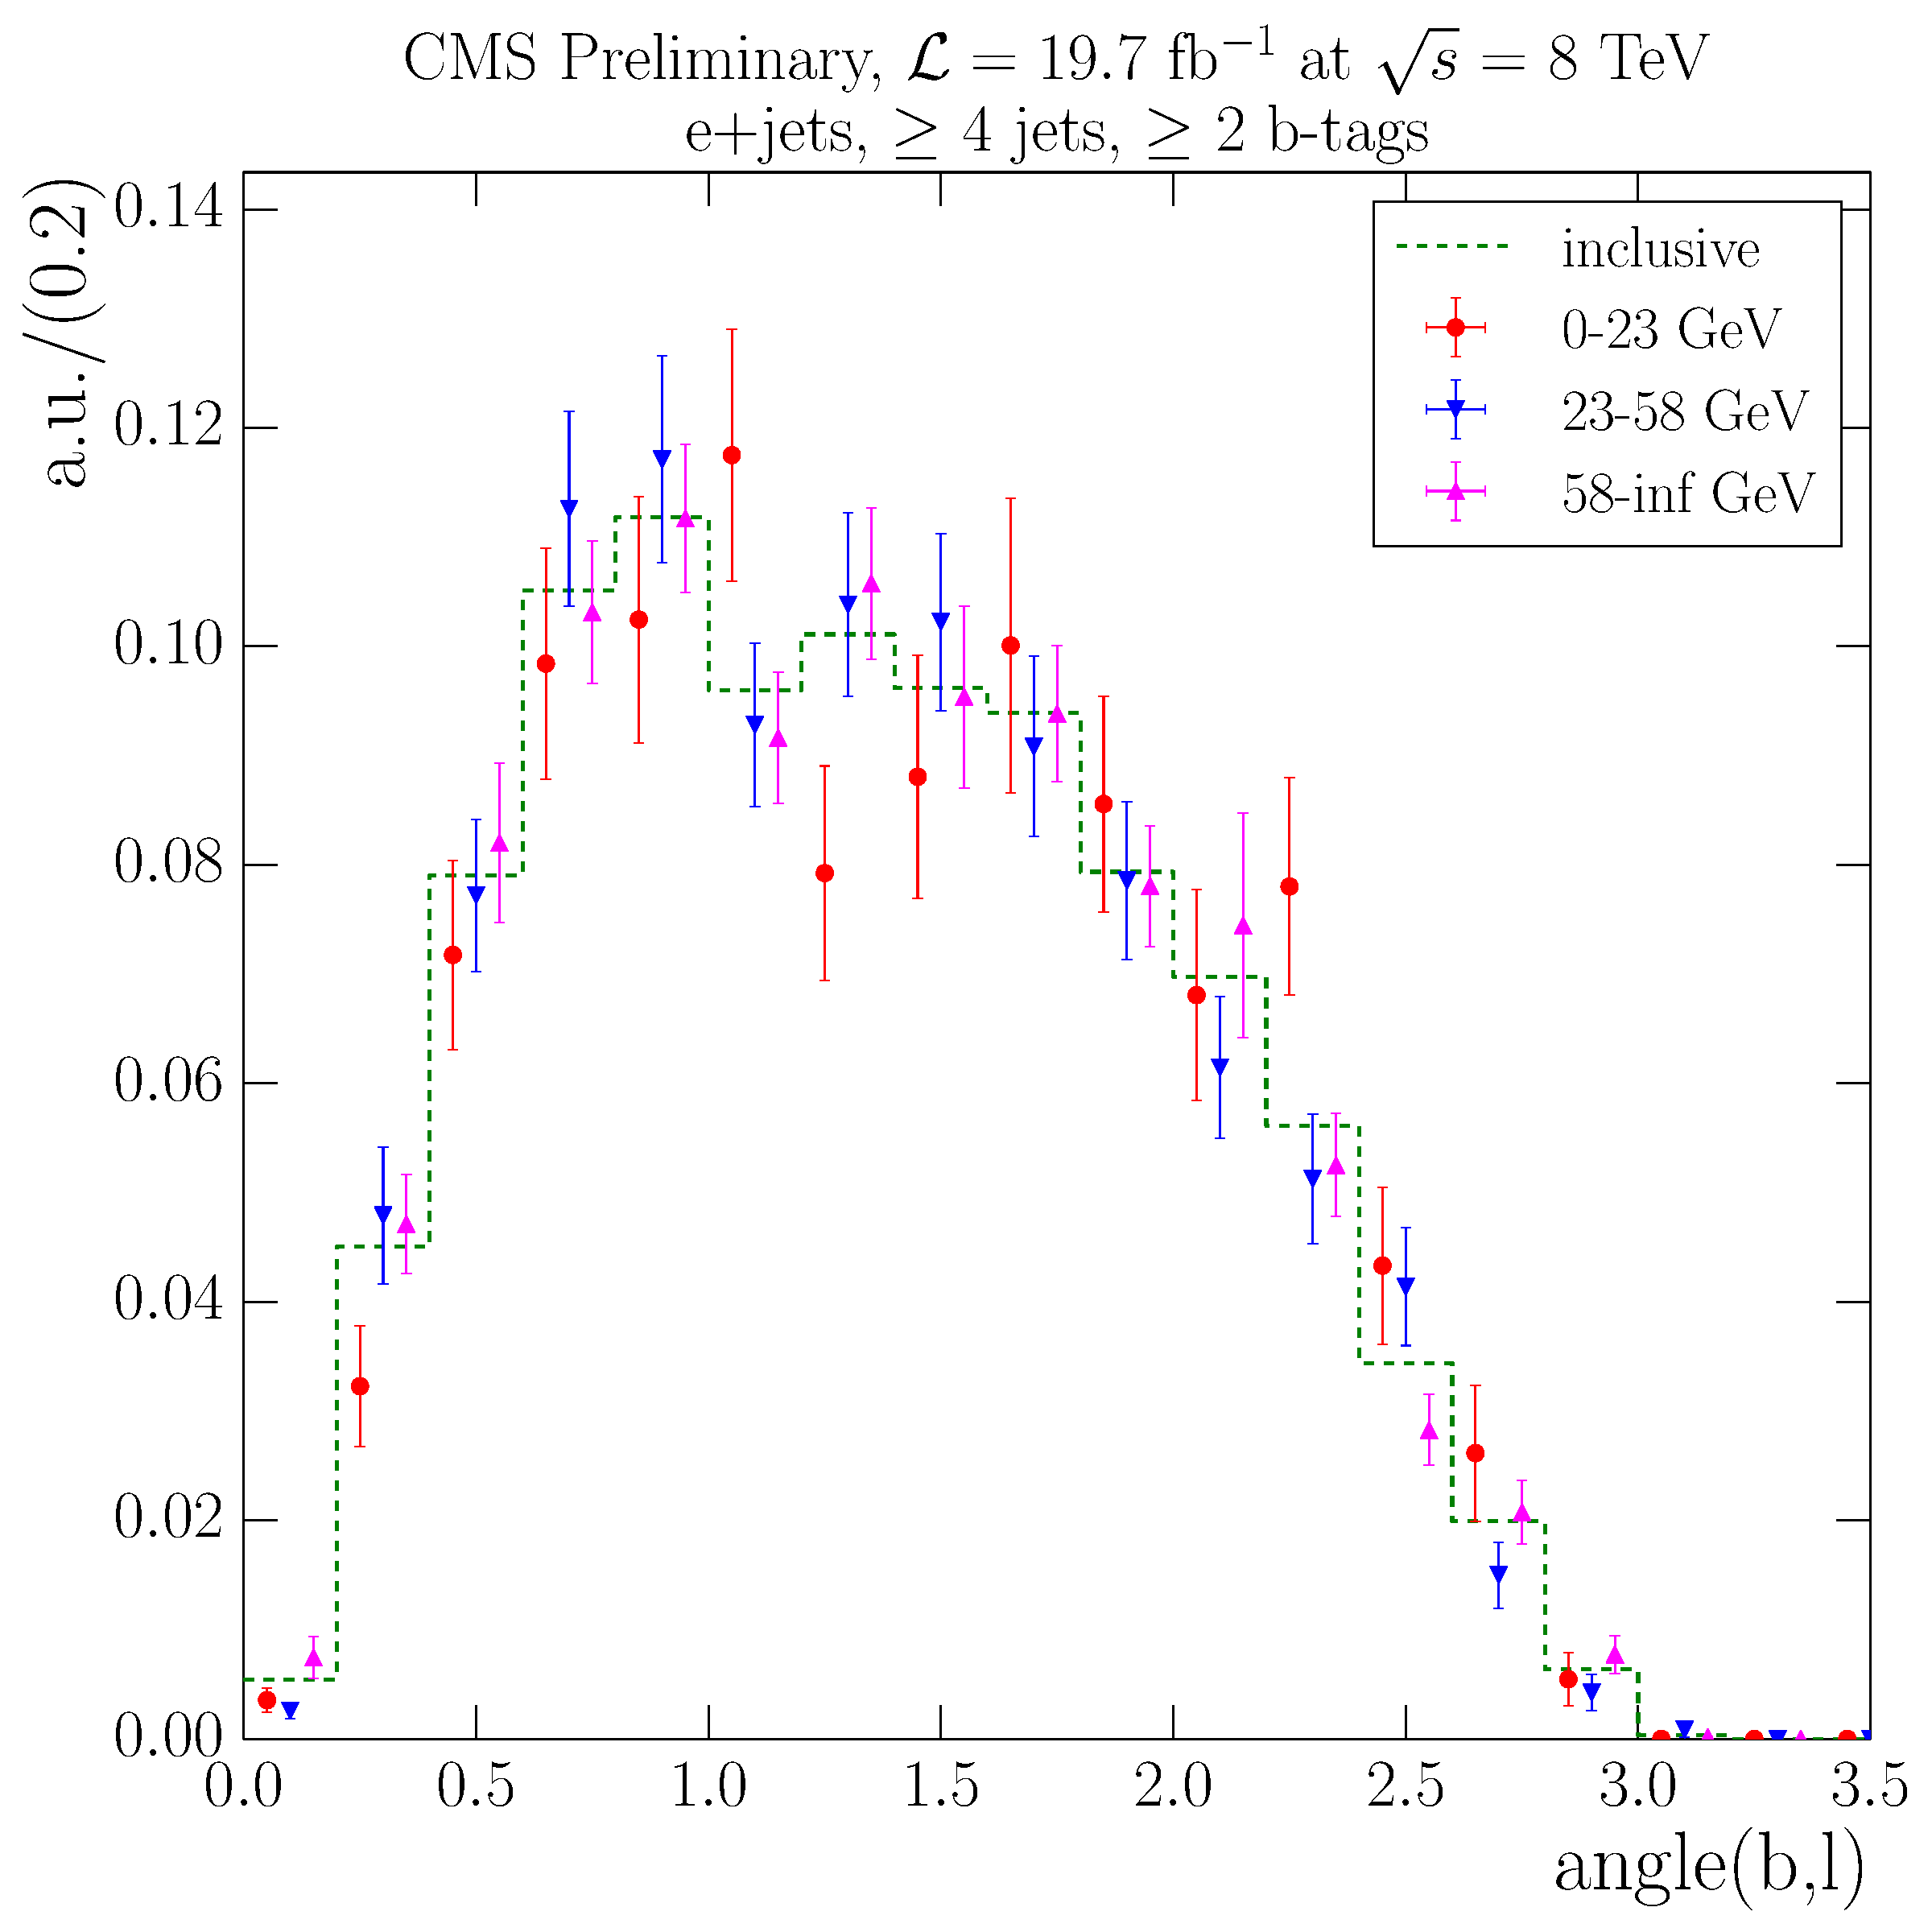
\includegraphics[width=0.48\textwidth]{Chapters/04_Analysis/04b_XSections/images/8TeV/fit_variables/MT/angle_bl/vjets/MT_angle_bl_2orMoreBtags_VJets_template_comparison.pdf}\hfill
     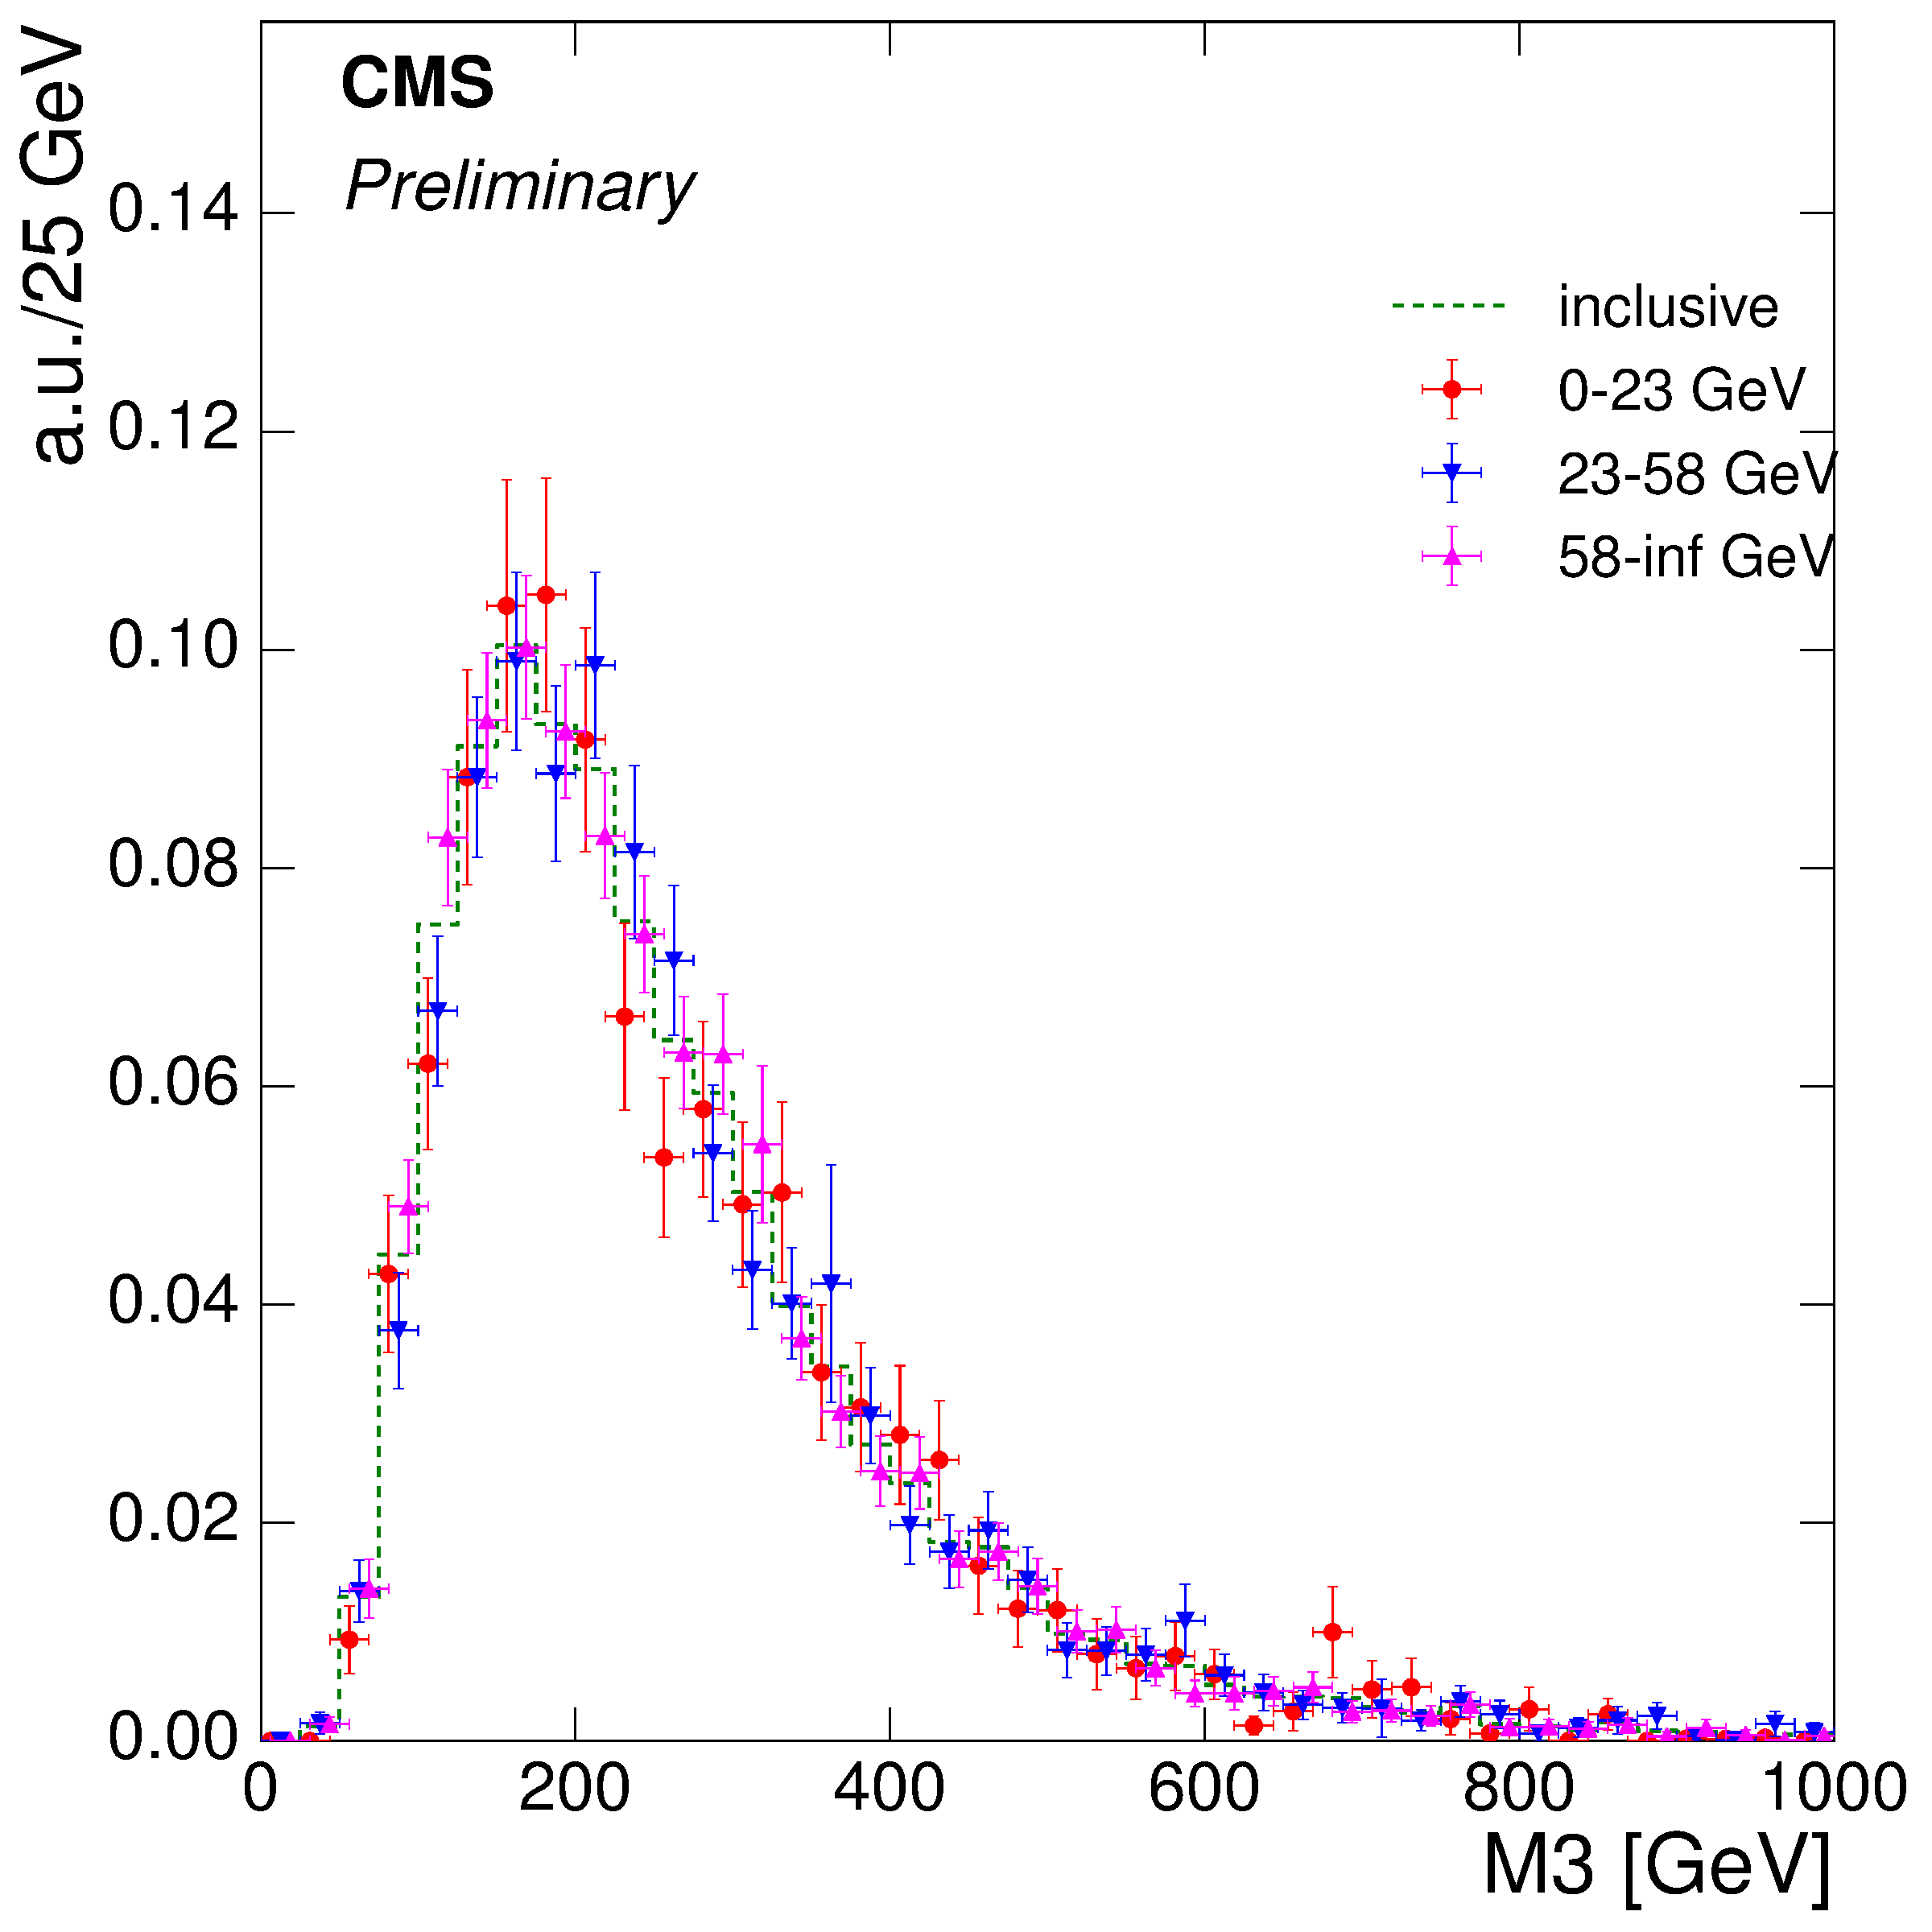
\includegraphics[width=0.48\textwidth]{Chapters/04_Analysis/04b_XSections/images/8TeV/fit_variables/MT/M3/vjets/MT_M3_2orMoreBtags_VJets_template_comparison.pdf}\\
	 \caption{Normalised distributions of the V+jets templates for the three fit variables at $\sqrt{s}=8\TeV$
	 inclusive across all \mt bins and for individual \mt bins: electron \abseta (upper
	 left), muon \abseta (upper right), $\alpha$ (lower left) and M3 (lower right).}
     \label{fig:MT_fit_variable_vjets_comparisons_8TeV}
\end{figure}

\begin{figure}[hbtp]
    \centering
     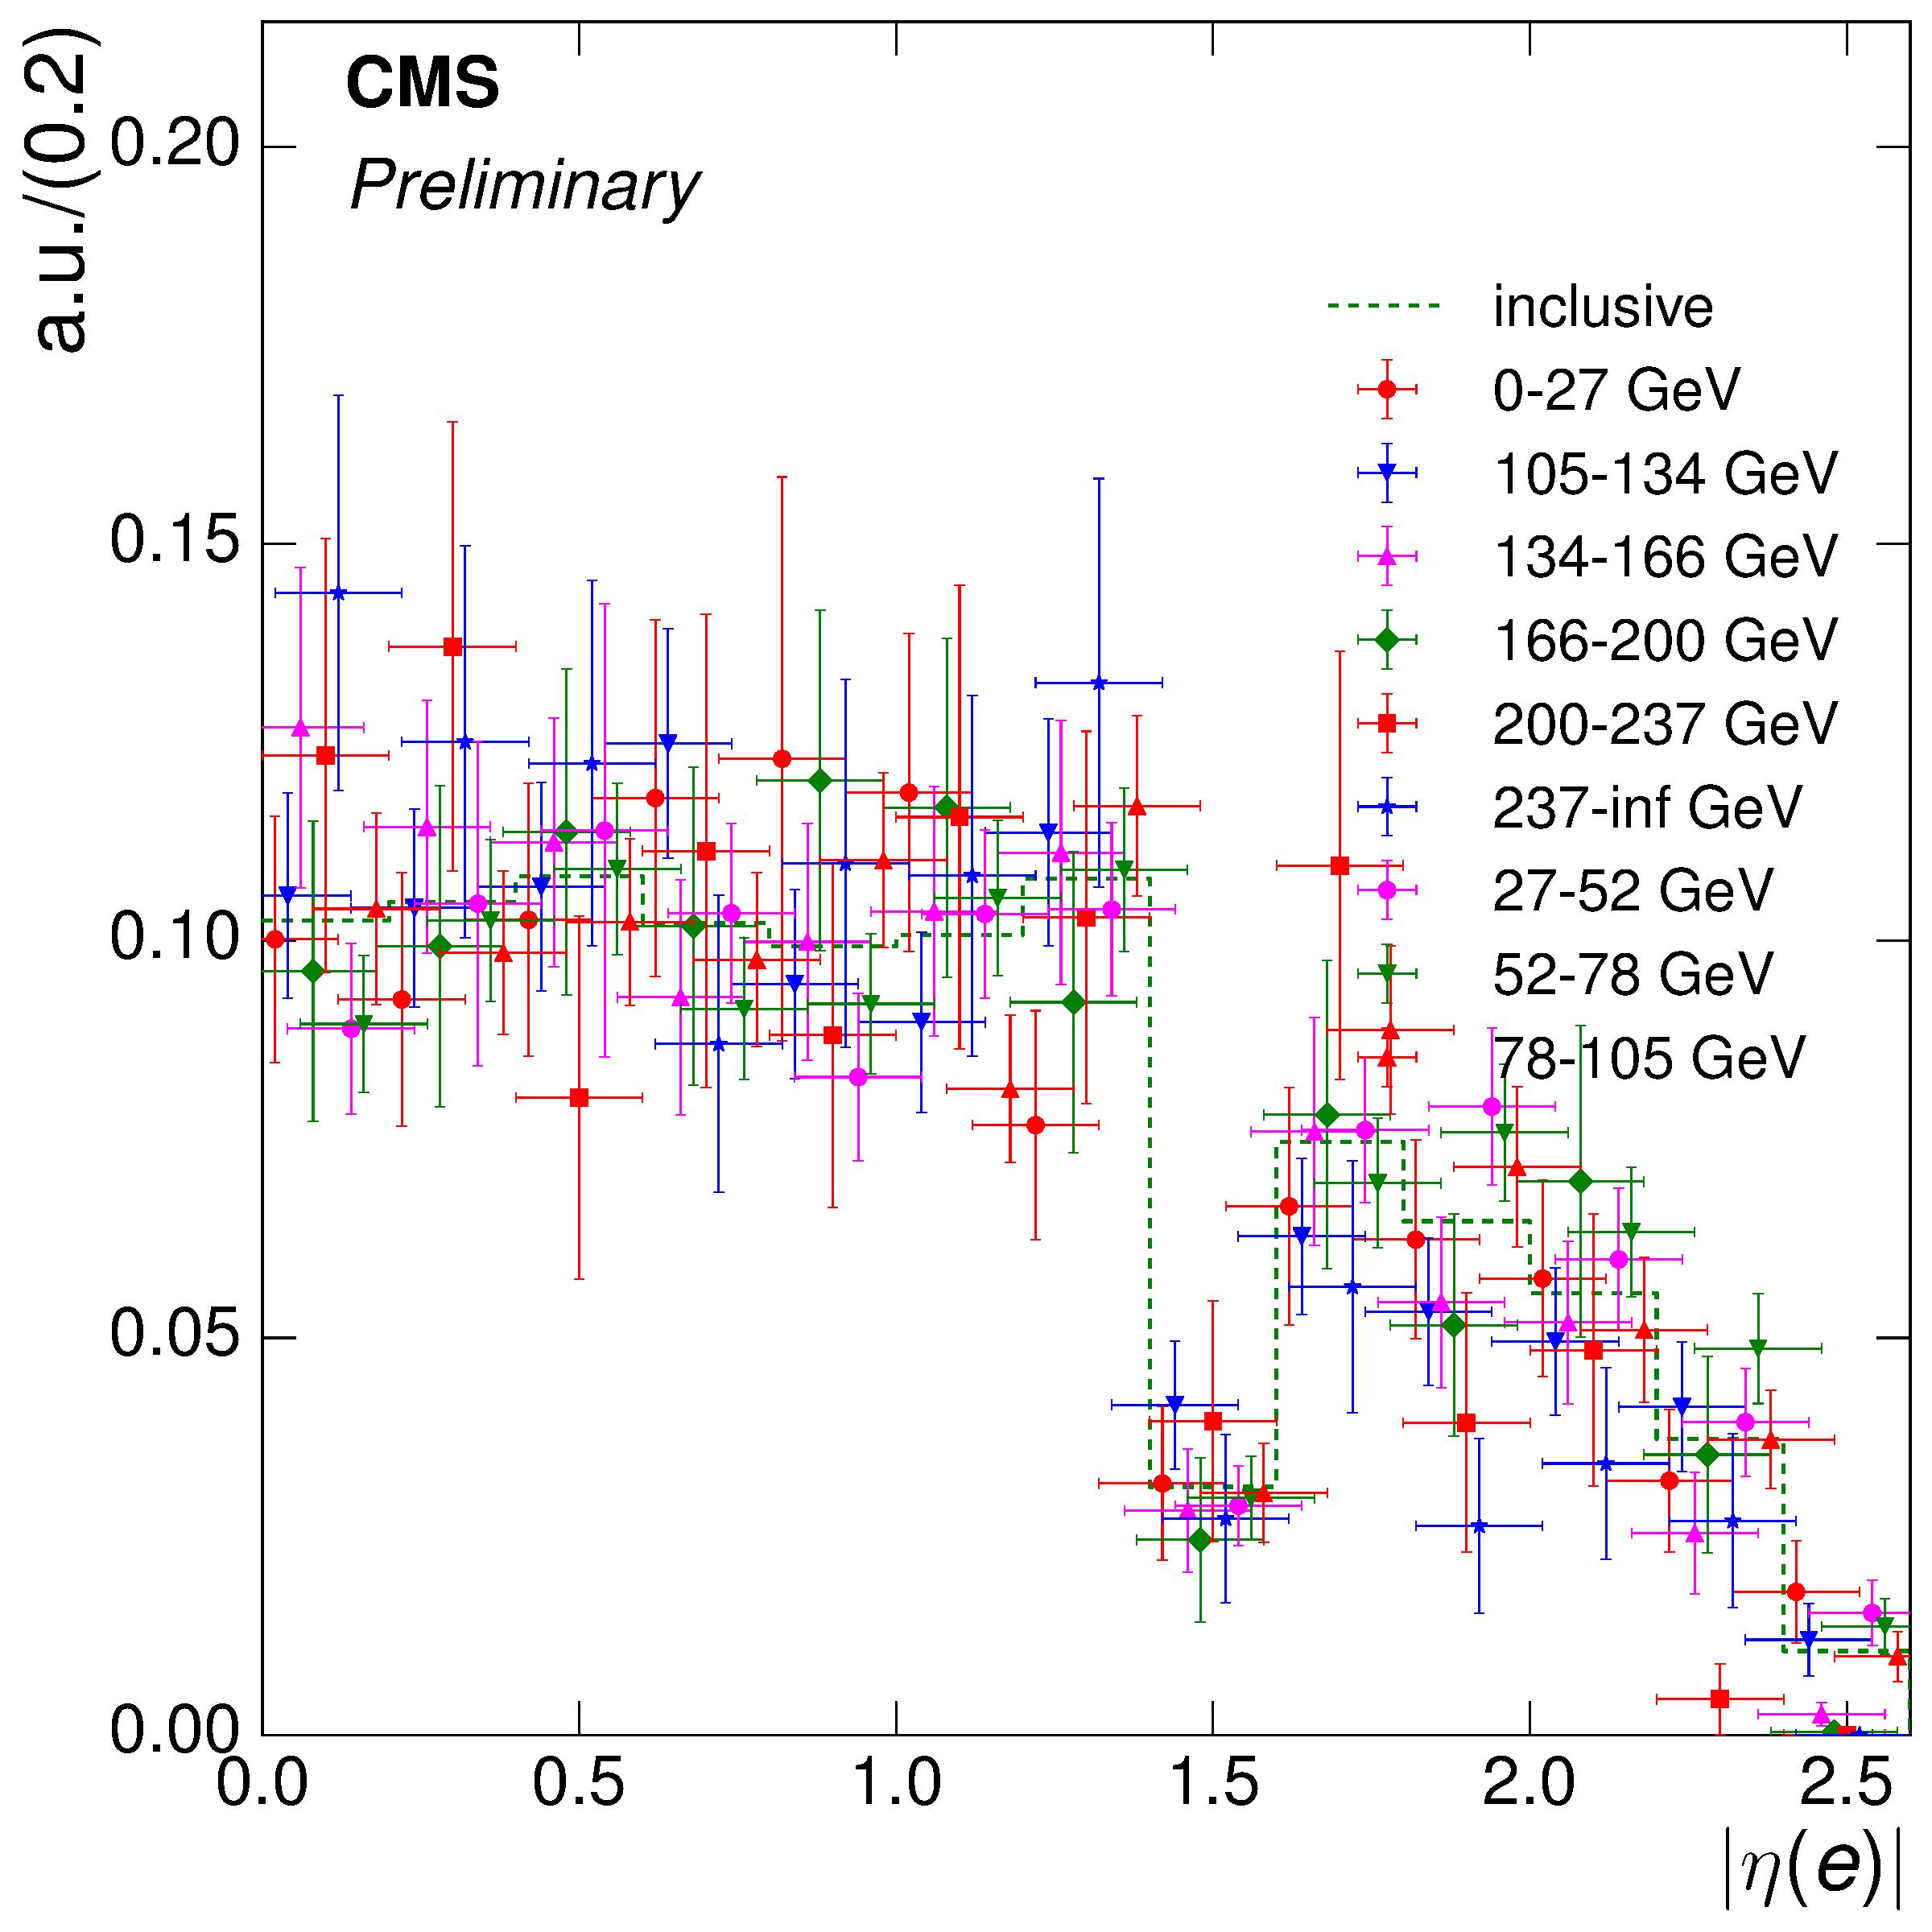
\includegraphics[width=0.48\textwidth]{Chapters/04_Analysis/04b_XSections/images/8TeV/fit_variables/WPT/electron_absolute_eta/vjets/WPT_electron_absolute_eta_2orMoreBtags_VJets_template_comparison.pdf}\hfill
     
\includegraphics[width=0.48\textwidth]{Chapters/04_Analysis/04b_XSections/images/placeholder.png}\\
     %\includegraphics[width=0.48\textwidth]{Chapters/04_Analysis/04b_XSections/images/7TeV/fit_variables/WPT/muon_absolute_eta/vjets/WPT_inclusive_muon_absolute_eta_2orMoreBtags_templates.pdf}\\
     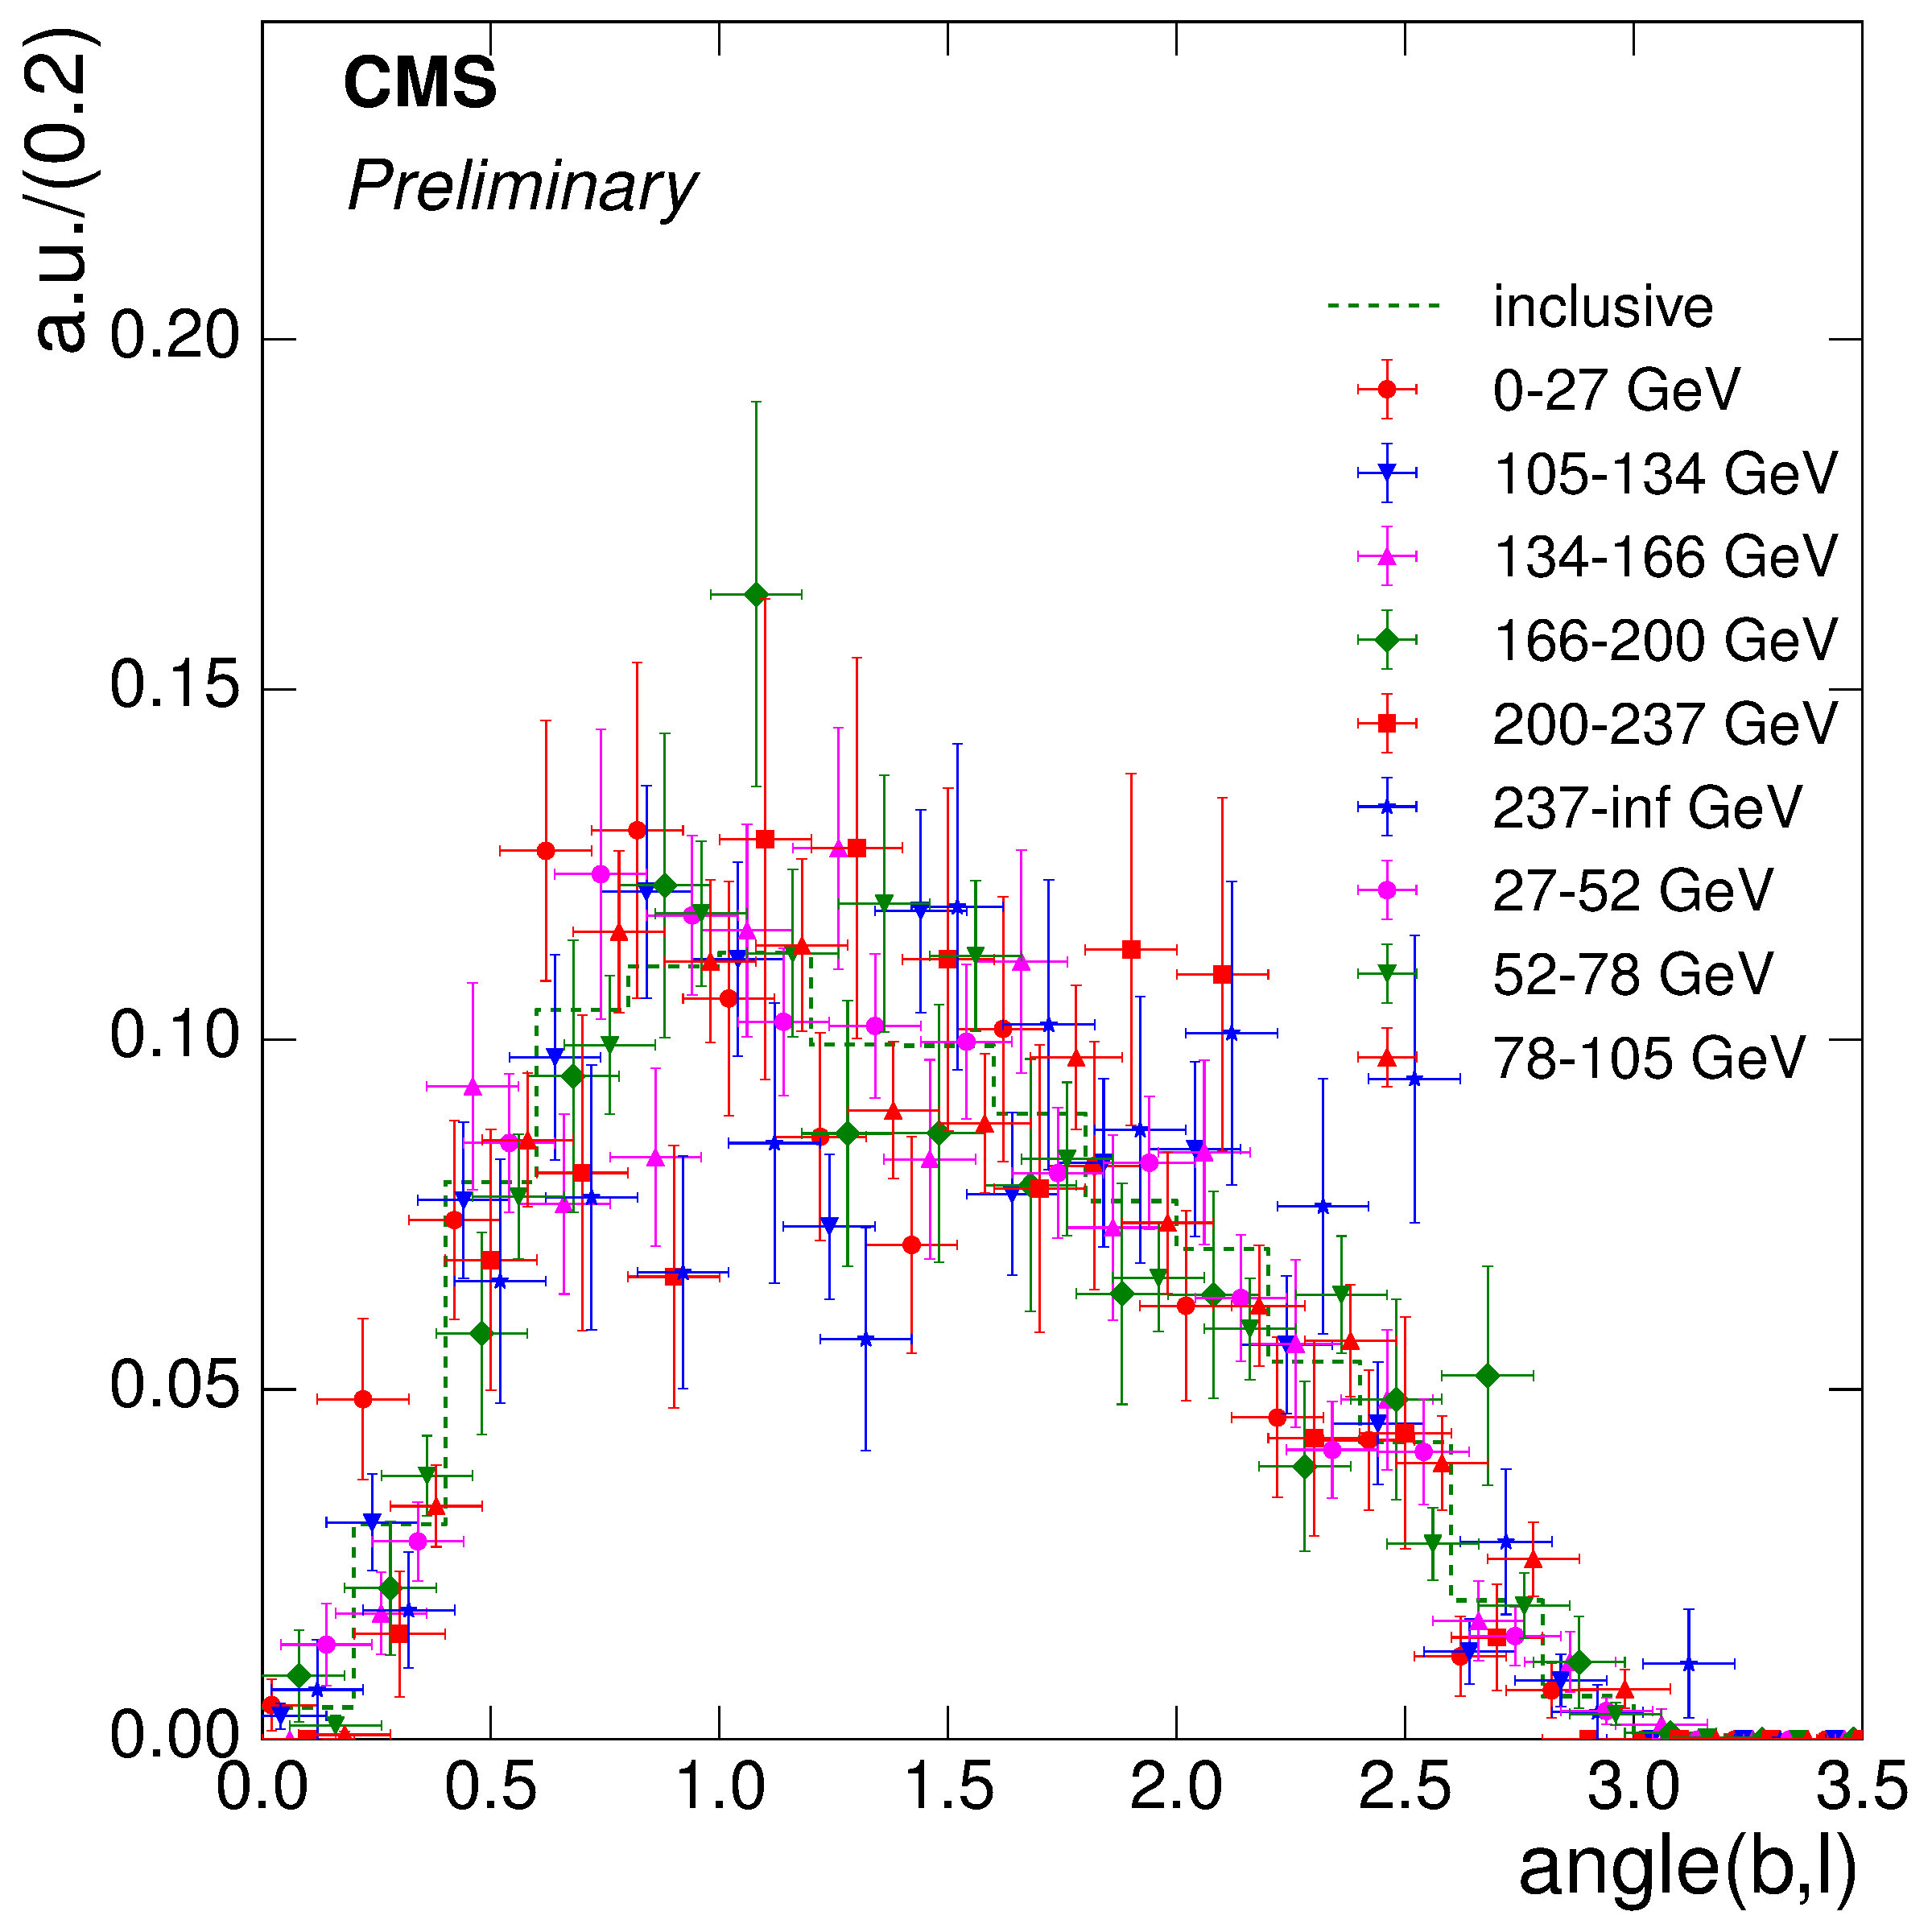
\includegraphics[width=0.48\textwidth]{Chapters/04_Analysis/04b_XSections/images/8TeV/fit_variables/WPT/angle_bl/vjets/WPT_angle_bl_2orMoreBtags_VJets_template_comparison.pdf}\hfill
     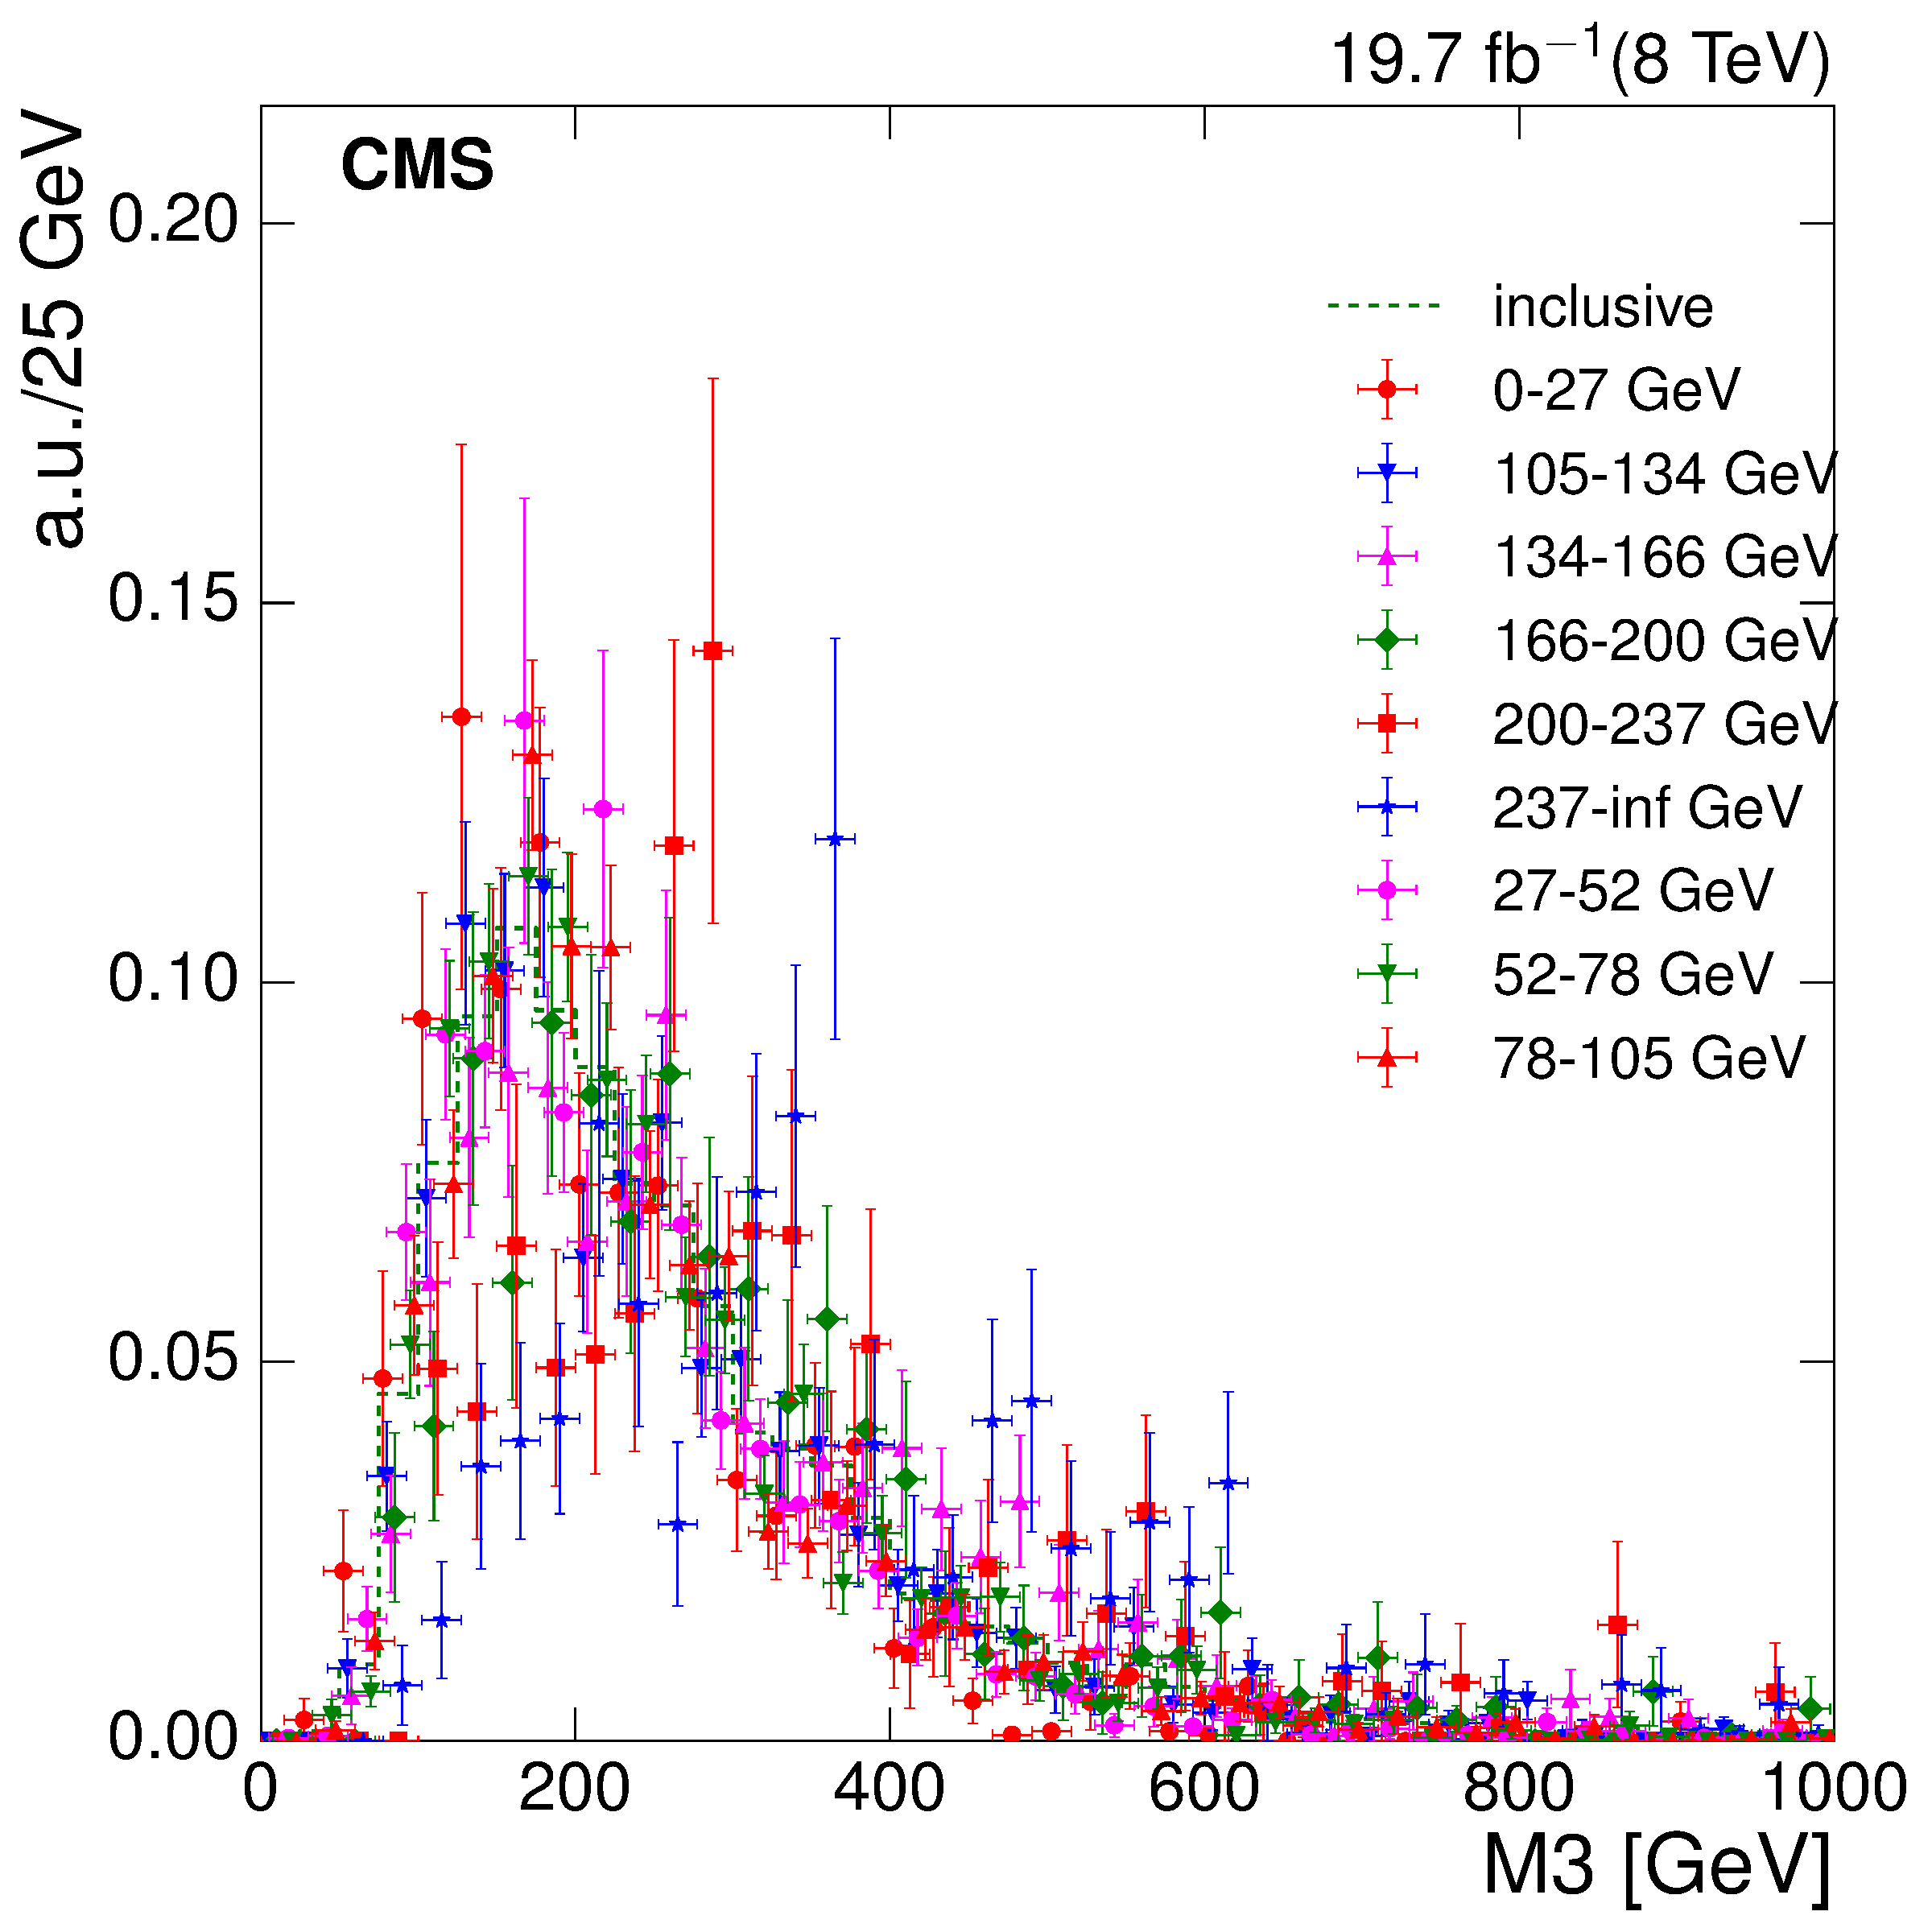
\includegraphics[width=0.48\textwidth]{Chapters/04_Analysis/04b_XSections/images/8TeV/fit_variables/WPT/M3/vjets/WPT_M3_2orMoreBtags_VJets_template_comparison.pdf}\\
	 \caption{Normalised distributions of the V+jets templates for the three fit variables at $\sqrt{s}=8\TeV$
	 inclusive across all \wpt bins and for individual \wpt bins: electron \abseta (upper
	 left), muon \abseta (upper right), $\alpha$ (lower left) and M3 (lower right).}
     \label{fig:WPT_fit_variable_vjets_comparisons_8TeV}
\end{figure}